\documentclass[
    iai, % Saisir le nom de l'institut rattaché
    mi, % Saisir le nom de l'orientation
    %confidential, % Décommentez si le travail est confidentiel
]{heig-tb}

\usepackage[nooldvoltagedirection,european,americaninductors]{circuitikz}
\usepackage[final]{pdfpages}
\usepackage{hyperref}
\DeclareMathSymbol{*}{\mathbin}{symbols}{"01}   % Replace "*" with middle point

\signature{Paillard.svg} % Remplacer par votre propre signature vectorielle.

%\makenomenclature
\makenoidxglossaries
\makeindex

\addbibresource{bibliography.bib}

\newacronym{ao}{AO}{Adaptative Optics}

\newglossaryentry{heig-vd}{
    name=HEIG-VD,
    description={Haute École d'Ingénierie et de Gestion du canton de Vaud}
}
\newglossaryentry{hes-so}{
    name=HES-SO,
    description={Haute École Supérieure de Suisse Occidentale}
}
\newglossaryentry{IRSOL}{
    name=IRSOL,
    description={Istituto ricerche solari Aldo e Cele Daccò}
}

\newglossaryentry{PSF}{
    name=PSF,
    description={Point spread function}
}

% Auteur du document (étudiant-e) en projet de Bachelor
\author{Ervan Paillard}

% Activer l'option pour l'accord du féminin dans le texte
\genre{male}

% Titre de votre travail de Bachelor
\title{Optical turbulence analyzer for the IRSOL telescope}

% Le sous titre est optionnel
\subtitle{Bachelor thesis}

% Nom du professeur responsable
\teacher {Prof. L.Jolissaint de Sepibus (HEIG-VD)}

% Mettre à jour avec la date de rendu du travail
\date{\today}

% Numéro de TB
\thesis{11112}



\surroundwithmdframed{minted}

%% Début du document
\begin{document}
\selectlanguage{English}
\maketitle
\frontmatter
\clearemptydoublepage
%\newpage

%% Requis par les dispositions générales des travaux de Bachelor
\pagenumbering{Roman}


\preamble
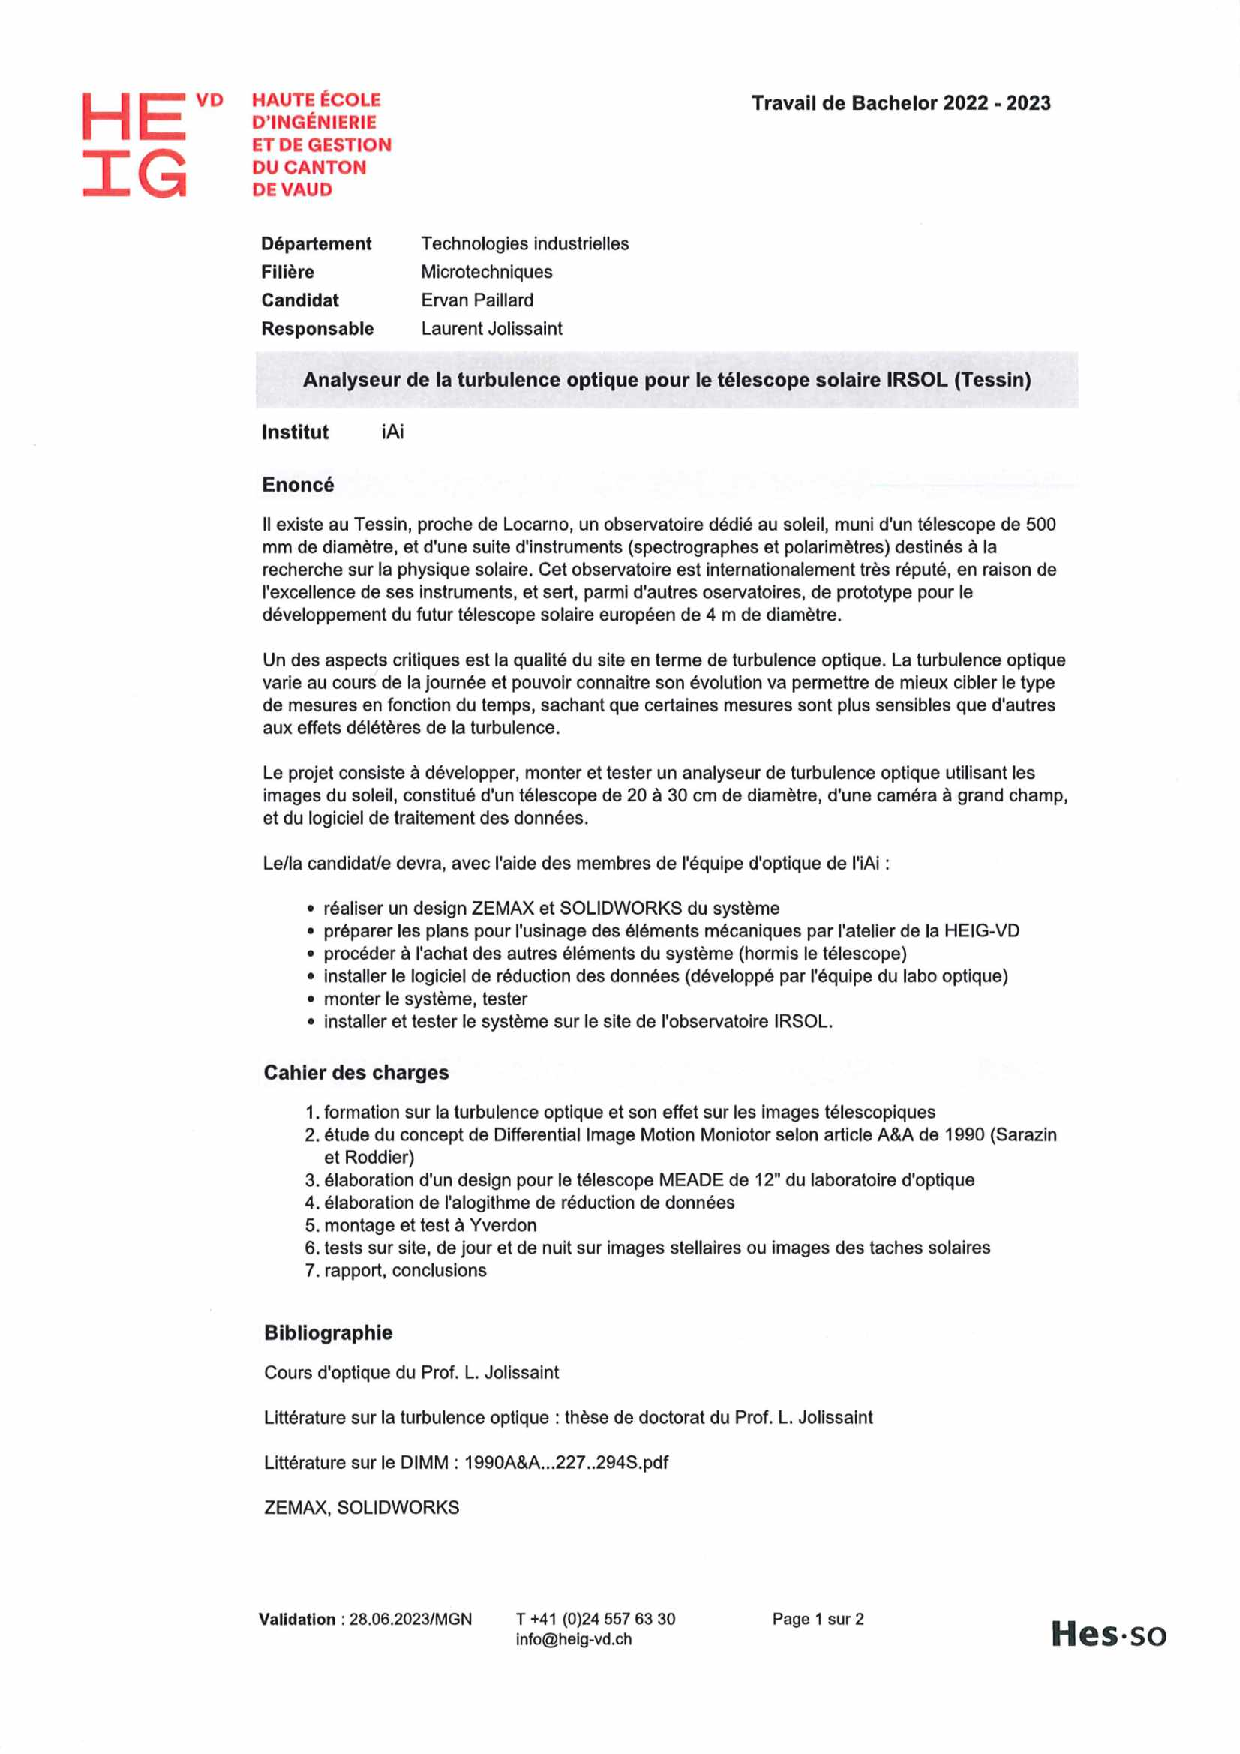
\includepdf[page=-,scale=0.9]{assets/figures/CDC/CahierDesCharges.pdf}
\Authentication

%% Résumé / Résumé publiable / Version abrégée
\begin{abstract}
    % Francais
% Cette thèse, en complément à une thèse réalisée en parrallèle, a été réalisée dans le but de caractériser le site 
% d'observation astronomique de IRSOL (Tessin).
% L'objectif est de quantifier la perturbations atmosphérique du site d'observation.
% L'outil qui a été sélectionné est un système appelé DIMM (Differential image motion monitor). 
% Le principe est simple. Il suffit de masquer une image en deux pour en faire une mesure différentielle. 
% La mesure différentielle permet d'annuler les perturbations extérieures qui pourraient apparaîtres autour du télescope 
% (par exemple les mouvements et vibrations)
% La perturbation atmosphérique induira des mouvements de cette image et le seeing se qualifiera grace à l'écart type de la mesure.
% Le résultat pourra être exprimé avec l'écart type de l'angle d'incidence des faisceau ($\sigma$) ou par le paramètre de Fried ($r_0$) correspondant.
% Le projet a été mené a bien en réalisant un design optique et mécanqiue pour une adaptation sur le télescope de la HEIG-VD.
% Un programme a été constitué afin de traiter les données de l'image et de quantifier la perturbation. 
% Les résultats ...

% English
This thesis, in addition to a parallel thesis, was carried out to characterize the IRSOL astronomical observation site (Ticino).
The aim is to quantify the atmospheric disturbance at the observation site. \newline
The tool selected was a system called DIMM (Differential image motion monitor).
It principle is simple, an image is masked in two to produce a differential measurement.\newline
Differential measurement cancels out any external disturbances that may occur around the telescope (e.g. movements and vibrations).
\bigbreak
Atmospheric disturbance will induce movements in this image, and the seeing will be qualified by the standard deviation of the measurement.
The result can be expressed as the standard deviation of the beam incidence angle ($\sigma$) or as the corresponding Fried parameter ($r_0$).
\bigbreak
The project was completed with an optical and mechanical design for adaptation to the \Gls{heig-vd} telescope.
A program was created to process the image data and quantify the disturbance. \newline
The results ...
\end{abstract}

%% Sommaire et tables
\clearemptydoublepage
%\newpage

{
    \tableofcontents
    \let\cleardoublepage\clearpage
    \listoffigures
}

\printnomenclature
\clearemptydoublepage
%\newpage

\printglossaries
\clearemptydoublepage
%\newpage

\pagenumbering{arabic}

%% Contenu
\mainmatter
\chapter{Introduction}
This chapter introduces the context and generalities relative to the work.

%====================================================================================================
% Context
%====================================================================================================
\section{Context}
This bachelor's thesis was carried out to support the research of the institute \Gls{IRSOL}. \newline
<<\Gls{IRSOL} is a research institute dependent on a foundation of the same name and affiliated to Università della Svizzera italiana.>>$^1$
The institute is based above Locarno in Ticino. \newline
Their research is mainly based on the measurement and characterization of the sun, and specializes in :
<<
\begin{enumerate}
    \item observational spectropolarimetry and instrument development,
    \item theoretical modeling of the generation and transfer of polarized radiation,
    \item numerical simulation of the solar atmosphere and numerical radiative transfer.
\end{enumerate}>>\footnote{|2| \Gls{IRSOL}, 2023. RESEARCH ACTIVITY, Research Activity at \Gls{IRSOL}. [Online]. [Accessed on 21.07.2023]. Available at: https://www.irsol.usi.ch/research/research-activity/}

The problem is that the institute is looking to expand its equipment in order to develop their research.
However, it is necessary to know the limitations of the measuring instruments, as well as the quality of the observation site.
Their first development objective would be to integrate an \acrfull{ao} system.
\newline
In odrer to asses the usefullness of \Gls{ao} two Bachelor thesis are conducted.
\begin{enumerate}
    \item "Caractérisation du télescope de l'observatoire solaire \Gls{IRSOL} (Tessin)" (Characterization of the \Gls{IRSOL} solar observatory telescope (Ticino))
    \item This thesis : "Analyseur de la turbulence optique pour le télescope solaire \Gls{IRSOL}" (Optical turbulence analyser for \Gls{IRSOL}'s solar telescope)
\end{enumerate}
The 1\textsuperscript{st} one is meant to measure the optical imperfections of the telescope itself and maybe of other optical equipment.
The 2\textsuperscript{nd} one aims to analyse optical turbulence on site.

Once these two projects are completed, \Gls{IRSOL} will be able to determine whether the acquisition of an \acrfull{ao} makes sense
and they will also be able to quantify the limiting element to their research (the observation site or the telescope).



%====================================================================================================
% Issue at hand
%====================================================================================================
\section{Issue at hand}
In a discussion with the institute, it was said: "Seeing evolves over the course of the day.
When the sun rises, the ground warms up and the heat rises. This is when seeing is at its worst.
But when the sun goes down, there's a moment when seeing is almost non-existent because the air currents freeze before going down again."
\bigbreak
The issue at hand is that the quality of the observation site is known but cannot be quantified.
The aim of this study is to quantify the quality of their observation site.
The instrument used will be the \Gls{DIMM} (Differential image motion monitor).

A \Gls{DIMM} works as follows (simplified version) :
\begin{enumerate}
    \item Capture an image masked by two small holes.
    \item Tracking the movement of these images.
    \item Measurement of the standard deviation of this movement.
    \item Conversion of previous result into turbulent layer thickness.
\end{enumerate}
The aim will be to play with the exposure time to determine the location of the image center, but also to freeze the turbulence.
\newline
Atmospheric turbulences will vary the centroid of the image, and it is this element that will be measured.
By taking the standard deviation of all these measurements, it is possible to give a result that qualifies the turbulence in a defined time.
\newline
The long explanation is the subject of this document.



\chapter{Theory}
%====================================================================================================
% Fundamentals
%====================================================================================================
\section{Fundamentals}
This parts goes over the fondamentals of optics necessary to understand futur developpments.
%====================================================================================================
% Seeing
%====================================================================================================
\subsection{Seeing}
\textbf{What's the seeing ?} : \newline In atmospheric optics, the "seeing" refers to the degree of blurring or distortion of astronomical objects
caused by Earth's atmosphere. The Earth's atmosphere is not homogeneous. It has various layers of air with different densities and temperatures.
Theses different layers causes the light passing throught it to be refracted in different ways. This result causes a constantly change of blurring,
distortion and glittering. Especially when looking an object low on the horizon. In our case, at IRSOL, the seeing is 4' of arc. We can go up
to 1' arc in the best case\newline
In general, seeing is determined by the angle of an object seen through the atmosphere, which is affected by factors such as temperature and wind speed.
The result of the seeing measure is the inverse of the "Fried parameter", wich describes the size of the atmospheric cells that cause the blurring.
When the Fried parameter is small, we could say that the seeing have good conditions. That means the image will have minimal blurring and distortion.
While poor seeing conditions have a larger Fried parameter, resulting in significant blurring and distortion of atmospherical objects.
%(Paramètre de Fried => Inverse)
\bigbreak
\textbf{Where are the turbulences} : \newline
First, we need to know how much type of turbulence we could see appearing and where they could be appear.\newline
There are 4 types of turbulence that we could see on the atmosphere. Each type is listed below :
\begin{itemize}
    \item Dome turbulence : \newline Appear when the air as not the same temperature between inside and outside the dome. This turbulence corresponds to
          the mirror turbulence.
    \item Surface trubulence : \newline Appear between the first 10 to 100 meters. Its appearance is due to the cooling by convection of the ground
          heated by the sun. Its minimum is just after the sunrise and its minimum when the sun sets. The evolution of this turbulence is an increasing
          evolution before the zenith and a decreasing evolution after it.\newline
          To counter this turbulence, a site selection is recommanded. For minimize it, the telescope could be place on a tower, away from any surface.
    \item Medium altitude turbulence : \newline Appear between 1.5 to 6 kilometers. Its appearance is due to atmospheric streams and in the thermal
          instabilities of the atmosphere. This turbulence is made up of multitudes of fine turbulent layers of varying densities and of a few hundred
          meters. For minimize it, a measure on the site should be carried out before.
    \item Tropopause and stratospheric turbulence : \newline Could appear between 6 and 20 kilometers. It reach a minimum t 6km and maximum on the
          tropopause between 10 and 20km. Its appearance is due to the strong winds shearing the atmosphere. This tubulence decrease after reach its maximum
          until it disappears after 25 - 30km.
\end{itemize}

%====================================================================================================
% DIMM
%====================================================================================================
\subsection{Differential image motion monitor (DIMM)}
\textbf{What's a DIMM ?} : \newline A differential image motion monitor is an instrument used in atmospheric optics to measure the amount of turbulence
in the Earth's atmosphere. It analyze the movement of stars as their light passes through the atmosphere, wich causes the stars to twinkle and blur.
\newline
The DIMM system consists of mask and split the image in two. After that, each image is recorded with a camera. On each part of this camera, the image
has a different seeing. Theses differences are used to determine the amount of distortion caused by the atmosphere.\newline
If we made a differential measure of theses images, we will get the atmospheric turbulence, wich is expressed as the seeing or the size of the
blurred image of a point source. \newline
The DIMM technique is widely used in astronomical observations, as it provides an objective and quantitative measure of the atmospheric turbulence,
which can affect the resolution and sensitivity of telescopes. It is also used in adaptive optics systems, where it is used to measure the atmospheric
turbulence in real-time, and to correct for the distortions using deformable mirrors.

\bigbreak
\textbf{Structures} : \newline the DIMM system is a relatively simple and robust instrument, which provides an accurate and objective measure of the atmospheric turbulence.
The elements that constitute a Differential Image Motion Monitor (DIMM) are listed below and viewable on the figure
\ref{fig:DIMM_Schematic} :
\begin{enumerate}
    \item Optical path : To create two images of our object, we need something wich will split our object in two. To realize this, a beam splitter could
          should be the best solution. It is also possible to separate the object before it enters the telescope by installing a "mask" before its first
          eyepiece.
    \item Camera : Which records the images of the star. The cameras are usually high-speed, sensitive detectors, such as CCDs or EMCCDs.
    \item Image processing software : The images obtained by the cameras are analyzed by software that measures the distortion caused by the atmosphere.
          The software calculates the difference in the distortion measurements obtained by the two telescopes, which allows for the determination of the
          atmospheric turbulence.
    \item Control and data acquisition system : The DIMM system is usually controlled by a computer, which also acquires and stores the data obtained by
          the cameras. The data can then be used to calculate the atmospheric turbulence, and to analyze the seeing conditions.
\end{enumerate}
\begin{figure}[H]
    \centering
    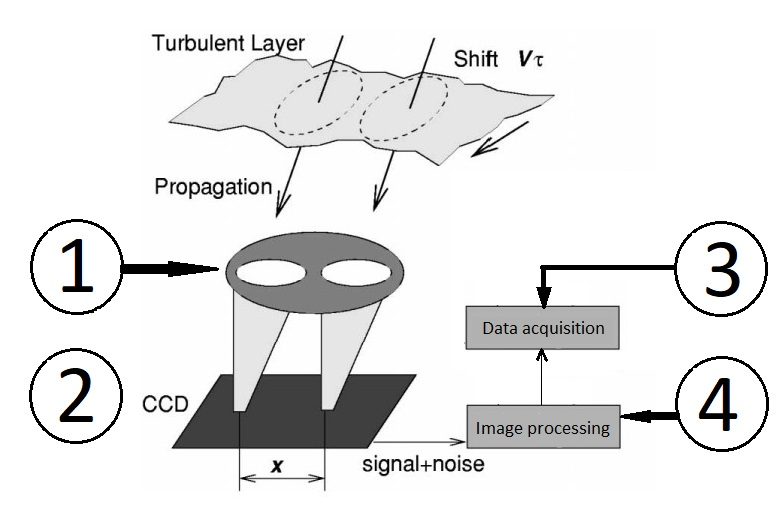
\includegraphics{assets/figures/Theory/DIMM_Schematic.jpg}
    \caption{Schematic principe of DIMM}
    \label{fig:DIMM_Schematic}
\end{figure}

\chapter{State of the art}
This chapter goes over a few solutions that already exist. Each aspect of the

\chapter{Optical design}
\section{Principe}
The principle of the optical design to be realized is schematized on the figure \ref{fig:OpticalPrincipe}.\bigbreak
The output beam of the telescope must be made parallel before the system can be installed. Once the beam is parallel,
a mask composed of 2 equal openings will limit it. This mask correspond to the entry of the system.\newline
The beam will enter to a prism which will deflect the beams to a lens.
The lens will intersept the 2 beams and allow to focus them on a sensor (BW camera).
\begin{figure}[H]
    \centering
    \includegraphics[scale=0.7]{assets/figures/Optical Design/Schéma optique.png}
    \caption{Optical schematic principe}
    \label{fig:OpticalPrincipe}
\end{figure}
\newpage
%====================================================================================================
%====================================================================================================
% Drawing rays with matlab
%====================================================================================================
%====================================================================================================
\section{Drawing rays with matlab}
This part will correspond to the mathematical research to draw the rays on a matlab program. To simplify the program,
the chosen method is to draw lines through 2 points. The calculated points are the following:
\begin{enumerate}
    \item Prism entry = ($X_{PE1,2,3,4},Y_{PE1,2,3,4}$)
    \item Prism exit = ($X_{PO1,2,3,4},Y_{PO1,2,3,4}$)
    \item Lens entry/exit = ($X_{L1,2,3,4},Y_{L1,2,3,4}$)
    \item Screen entry = ($X_{S12,34},Y_{S12,34}$)
\end{enumerate}
Known data :
\begin{itemize}
    \item Prism angle = $\alpha$ [$\deg$] (converted into radian for the equations)
    \item Deflection of the incident beam = $i$ [" arc] (converted into radian for the equations)
    \item focal lens = $F$ [mm]
    \item Hole diameter = $d$ [mm]
    \item Distance betweeen two holes = $e$ [mm]
    \item Distance between the prism and the lens = $E$ [mm]
    \item Refractive index of the prism = $n_p$ [-]
    \item Prism width = $t_c$ [mm]
    \item Prism height = $h$ [mm]
\end{itemize}
Needed data :
\begin{itemize}
    \item Screen height = $H$ [mm]
    \item System length = $L$ [mm]
\end{itemize}
\newpage
%====================================================================================================
% Prism
%====================================================================================================
\subsection{Prsim}
\begin{figure}[H]
    \centering
    \includegraphics[scale=0.8]{assets/figures/Optical Design/Schéma prisme.png}
    \caption{Schematic of drawing rays at the input of the prism}
    \label{fig:Prism_Schematic}
\end{figure}
First, set the X and Y input coordinates.
\begin{equation}
    X_{PE1} = X_{PE2} = X_{PE3} = X_{PE4}
\end{equation}
\begin{equation}
    Y_{PE1} = \frac{e + d}{2} \newline
    Y_{PE2} = \frac{e - d}{2} \newline
    Y_{PE3} = \frac{-e - d}{2} \newline
    Y_{PE4} = \frac{-e + d}{2}
\end{equation}
Using Snell's law and the relationships between the angles, the exit angle can be determined.
\begin{equation}
    r = \arcsin(\frac{\sin(i)}{n_p})
\end{equation}

\begin{equation}
    \beta = \arcsin(n_p*\sin(\alpha-\arcsin(\frac{\sin(i)}{n_p})))-\alpha
\end{equation}
To find the output values, the affine line function (\ref{eq:DoiteAffine}) is used.
This requires knowledge of the slopes and offsets of the straight lines (beam + prism output face).
\begin{equation}
    m_1 = \frac{-1}{\tan(\frac{\pi}{2}-r)}\newline
    m_2 = \frac{-1}{\tan(\alpha)}
\end{equation}
\begin{equation}
    m_3 = \frac{-1}{\tan(\frac{\pi}{2}-r)}\newline
    m_4 = \frac{1}{\tan(\alpha)}
\end{equation}
\begin{equation}
    b_1 = Y_{PE1}-X_{PE1}*m_1\newline
    b_2 = Y_{PE2}-X_{PE2}*m_2\newline
    b_{1s} = \frac{h}{2}-t_e*m_2
\end{equation}
\begin{equation}
    b_3 = Y_{PE3}-X_{PE3}*m_3\newline
    b_4 = Y_{PE4}-X_{PE4}*m_4\newline
    b_{2s} = \frac{-h}{2}-t_e*m_4
\end{equation}
Now that the line parameters are known, the X and Y output points of each beam can be calculated.
\begin{equation}
    X_{PO1} = \frac{b_{1s}-b_1}{m_1-m_2}\newline
    Y_{PO1} = X_{PE1}*m_1+b_{1s}
\end{equation}
\begin{equation}
    X_{PO2} = \frac{b_{1s}-b_2}{m_1-m_2}\newline
    Y_{PO2} = X_{PE2}*m_2+b_{1s}
\end{equation}
\begin{equation}
    X_{PO3} = \frac{b_{2s}-b_1}{m_1-m_2}\newline
    Y_{PO3} = X_{PE1}*m_1+b_{1s}
\end{equation}
\begin{equation}
    X_{PO2} = \frac{b_{1s}-b_2}{m_1-m_2}\newline
    Y_{PO2} = X_{PE2}*m_2+b_{1s}
\end{equation}
Once the X,Y coordinates of the prism's inputs and outputs are known, it's easy to plot them in matlab (Appendix \ref{App:Matlab}).
%====================================================================================================
% Lens
%====================================================================================================
\subsection{Lens}
\begin{figure}[H]
    \centering
    \includegraphics{assets/figures/Optical Design/Schéma sortie prisme.png}
    \caption{Schematic of drawing rays at the output of the prism}
    \label{fig:PrismLens_Schematic}
\end{figure}
First, let's say :
\begin{equation}
    X_L = E
\end{equation}
With the equation of the affine line (\ref{eq:DoiteAffine}),
where "a" can be determined using trigonometry (\ref{eq:Trigo_tan}),
The offset can be determined using the points previously obtained.
\begin{equation}
    a = \frac{-1}{tan(90-\beta)}
\end{equation}
\begin{equation}
    Y_{out} = a*X_{out} + b ==> b = Y_{out} - a*X_{out}
\end{equation}
We can now pose the equation that determines the $Y_L$ coordinate
\begin{equation}
    Y_{L} = a*X_{L} + b
\end{equation}
Once the X,Y coordinates of the lens's inputs are known, and with the prism's output coordinates, it's easy to plot them in matlab (Appendix \ref{App:Matlab}).
\subsection{Screen}
\begin{figure}[H]
    \centering
    \includegraphics{assets/figures/Optical Design/Schéma Lentille.png}
    \caption{Schematic of drawing rays at the output of the lens}
    \label{fig:Lens_Schematic}
\end{figure}
To begin with, the X coordinate can be set as it corresponds to the focal
point of the lens. Note that this equation is only valid if the lens is approximated to a thin lens.
\begin{equation}
    X = E+F
\end{equation}
Then, thanks to trigonometry (\ref{eq:Trigo_tan}), it is easy to find the coordinates Y
\begin{equation}
    Y = \pm F*tan(\beta)
\end{equation}
Once the X,Y coordinates of the screen's inputs are known, and with the lens's output coordinates, it's easy to plot them in matlab (Appendix \ref{App:Matlab}).
%====================================================================================================
%====================================================================================================
% Matrice de conjuguaison avec matlab
%====================================================================================================
%====================================================================================================
\newpage
\section{Conjugation matrix with matlab}
blblalbalblabl
%====================================================================================================
%====================================================================================================
% Mask sizing
%====================================================================================================
%====================================================================================================
\section{Mask sizing}\label{sec:Opti_Couille}
In order to know the mask size required to sample the image, we first need to know the size of the telescope's exit pupil.
\begin{figure}[H]
    \centering
    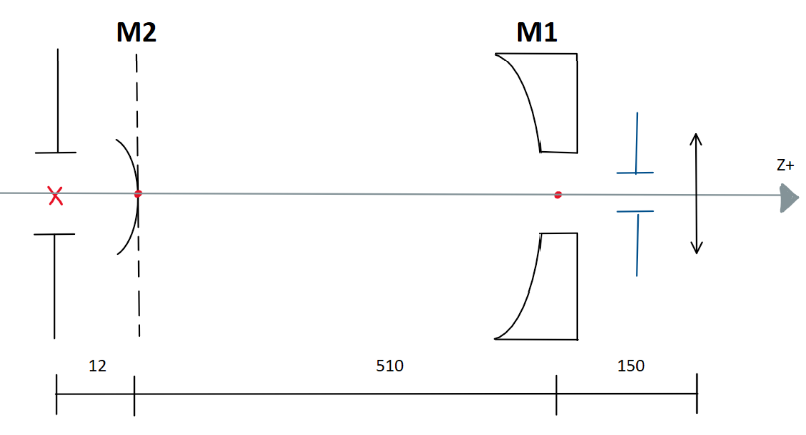
\includegraphics[scale=0.55]{assets/figures/Optical Design/Design_Mask.png}
    \caption{Selected camera}
    \label{fig:Opti_Mask_Diagram}
\end{figure}
%====================================================================================================
%====================================================================================================
% Camera specifications
%====================================================================================================
%====================================================================================================
\section{Camera specifications}\label{sec:Opti_Cam}
\subsection{Limitations}
In order to determine which sensor will have the right specifications for this application,
several elements will need to be calculated :
\begin{itemize}
    \item Pixel size to ensure an image with sufficient information
    \item Screen size
    \item The size the image will occupy on the sensor
\end{itemize}
\bigbreak
To begin with, the mask must be positioned at the telescope entrance. To do this, the relationship between
the holes and their spacing is used (:::). A virtual mask is placed over the telescope entrance,
with a 20mm margin taken on the sides (10mm each). Using these elements, the diameter of the holes on the
telescope can be determined by the equation \ref{eq:DMT} with $D_{MT}$ = diameter of a hole on the telescope entrance,
$D$ = diameter of the telescope, $margin$ = 20mm, $ratio$ = ratio between the holes and their spacing.
\begin{equation}\label{eq:DMT}
    D_{MT} = \frac{(D-margin)}{(ratio + 1)} = \frac{(305-20)}{5+1} = 47.5 mm
\end{equation}
Now we need to know the transverse magnification ($G_t$) between the holes in the mask and the virtual holes in the telescope.
This magnification will later be used to determine the available FOV.
\begin{equation}
    G_t = \frac{D_{holes}}{D_{MT}} = \frac{1}{47.5} = 0.0211
\end{equation}
\textbf{\textcolor{red}{Truc du sigma}}
\newline
Once the $\sigma_T$ is known, the fov as seen through the telescope can be determined. In equation \ref{eq:FOV_T}, $D_S$ is the diameter
of the sunspots to be measured (20").
\begin{equation}\label{eq:FOV_T}
    FOV_T = 6 * \sigma_T + D_S
\end{equation}
Once the FOV seen by the telescope is known, this parameter must be transferred to the mask.
\begin{equation}
    FOV_M = FOV_T * G_t^{-1}
\end{equation}
This FOV will be converted into a radiant and can then be transferred to the CMOS sensor
using the lens focal length ($F$) determined in section \ref{sec:Opti_Lens}.
\begin{equation}
    FOV_S = FOV_M * F
\end{equation}
Finally, the three elements listed at the beginning of this section can be calculated.
\begin{itemize}
    \item The maximum pixel size of the CMOS sensor must respect Niquist's theorem.
          \begin{equation}
              pixel_{max} = \frac{\lambda*F}{2*D_{holes}}
          \end{equation}
    \item The number of pixels in an image will be :
          \begin{equation}
              N_{p} = \frac{FOV_S}{pixel_{max}}
          \end{equation}
    \item The minimum screen size required to view the 2 images (assuming they are centered) is :
          \begin{equation}
              Screen_{Size} = (\frac{H}{pixel_{max}}+ N_{p}*2);
          \end{equation}
\end{itemize}
For the 3 points above, calculations were performed using matlab (Appendix \ref{App:Matlab}) and worst-case scenarios
were considered. Calculations were made for a value of $r_0$ ranging from 0.02m to 0.2m.
Based on these calculations, the following results were obtained:
\begin{itemize}
    \item Maximum pixel size : 15 [$\mu$m]
    \item Minimum screen size : 164 [pixel]
    \item Size of one image : 17 [pixel]
\end{itemize}
\subsection{Choice}
With the specifications calculated above and after some research, the camera shown in figure 2 was chosen.
\begin{figure}[H]
    \centering
    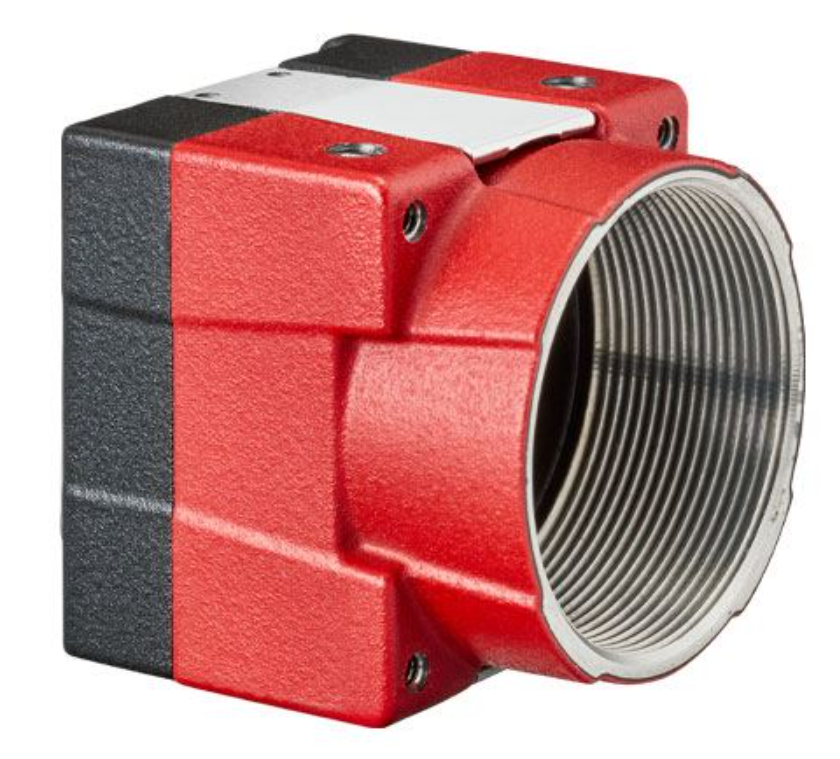
\includegraphics[scale=0.35]{assets/figures/Mechanical Design/Camera.png}
    \caption{Selected camera}
    \label{fig:Camera2}
\end{figure}
The camera in figure \ref{fig:Camera2} is an Allied vision camera (Alvium 1800 U-052m). This camera is
equipped with a monochromatic CMOS sensor (Sony IMX426). Its pixels are 9x9 [$mu$m], its size is 816x624 [pixel]
and this camera is capable of exposure times from 21 $mu$s to 10s.
\bigbreak
With this camera, an image will take up around 28 pixels and the total image will be 250 pixels long.
If the total image is centered on the sensor, camera orientation will have no effect on the measurement.
The image should always be on the sensor.
%====================================================================================================
%====================================================================================================
% Lens selection
%====================================================================================================
%====================================================================================================
\newpage
\section{Lens selection}\label{sec:Opti_Lens}
The choice of lens is one of the critical elements of this project. Several parameters need to be taken
into account, such as \gls{PSF} on the focal plane, Zernik polynomials and the correct Strehl ratio.
The validation method for the use of a certain lens was a simulation on Zemax.
In order to best reproduce the system, an angle on the incident beam had to be added.
This angle corresponds to the beam deflection produced by the prism. The wavelength will also have to be modified to work at 600nm.
\begin{figure}[H]
    \centering
    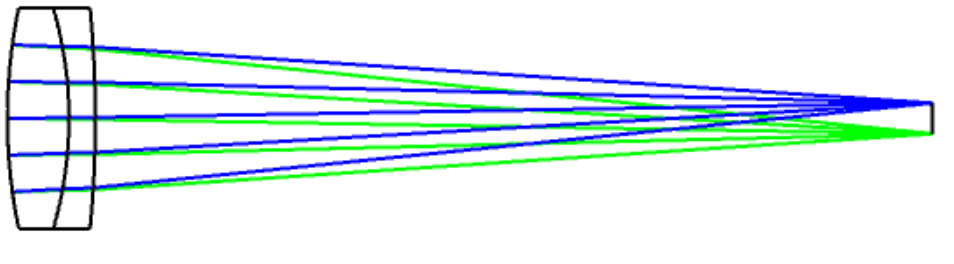
\includegraphics[scale=0.8]{assets/figures/Optical Design/Zemax_RayTrace.png}
    \caption{Drawing of lens rays on Zemax}
    \label{fig:Opti_LensRayTrace}
\end{figure}
In order to maximize the system's critical parameters, it is essential to optimize the system when
the fields have not yet been introduced.
Once the system has been optimized, the beam angle can be entered in the "Data field editor".
\begin{figure}[H]
    \centering
    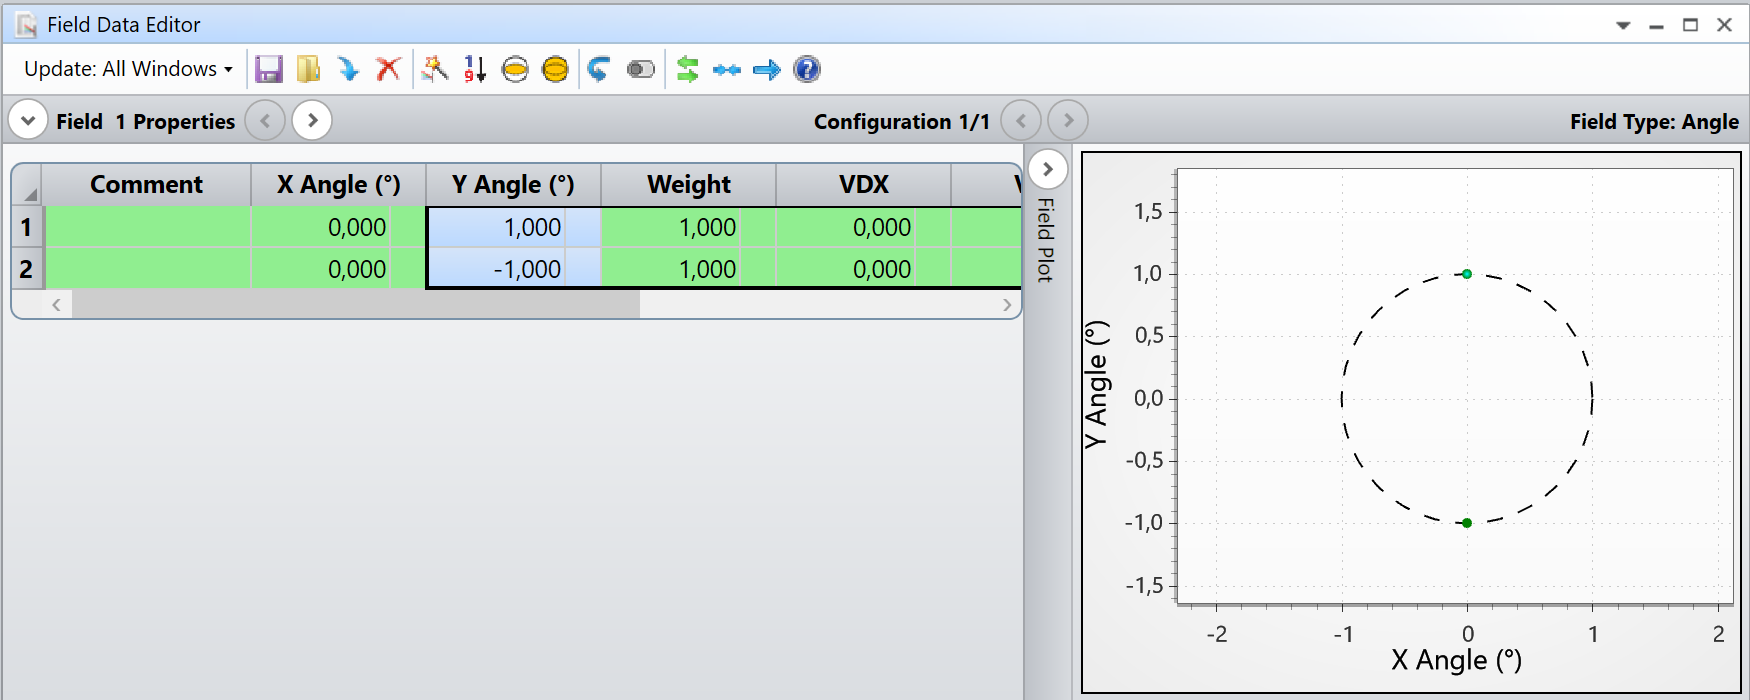
\includegraphics[scale=0.5]{assets/figures/Optical Design/Zemax_FieldEditor.png}
    \caption{zemax parameter window : "Field data Editor"}
    \label{fig:Opti_FieldZemax}
\end{figure}
Now that the parameters have been entered, all that remains is to analyze the results.
\newpage
\subsection{Point Spread Function}
The \gls{PSF} is the most critical element of optical design. It determines the image quality of the lens.
A good \gls{PSF} is characterized by a large peak centered in position (0,0) and a low spread of the function.
\newline
In Figure \ref{fig:Opti_ZemaxPSF}, the \gls{PSF} has a correct shape and its maximum rises to 0.875. This \gls{PSF} is completely acceptable
for the DIMM lens. It is that of the lens chosen (F=50mm) with a beam incidence angle of 1$^{\circ}$.
\begin{figure}[H]
    \centering
    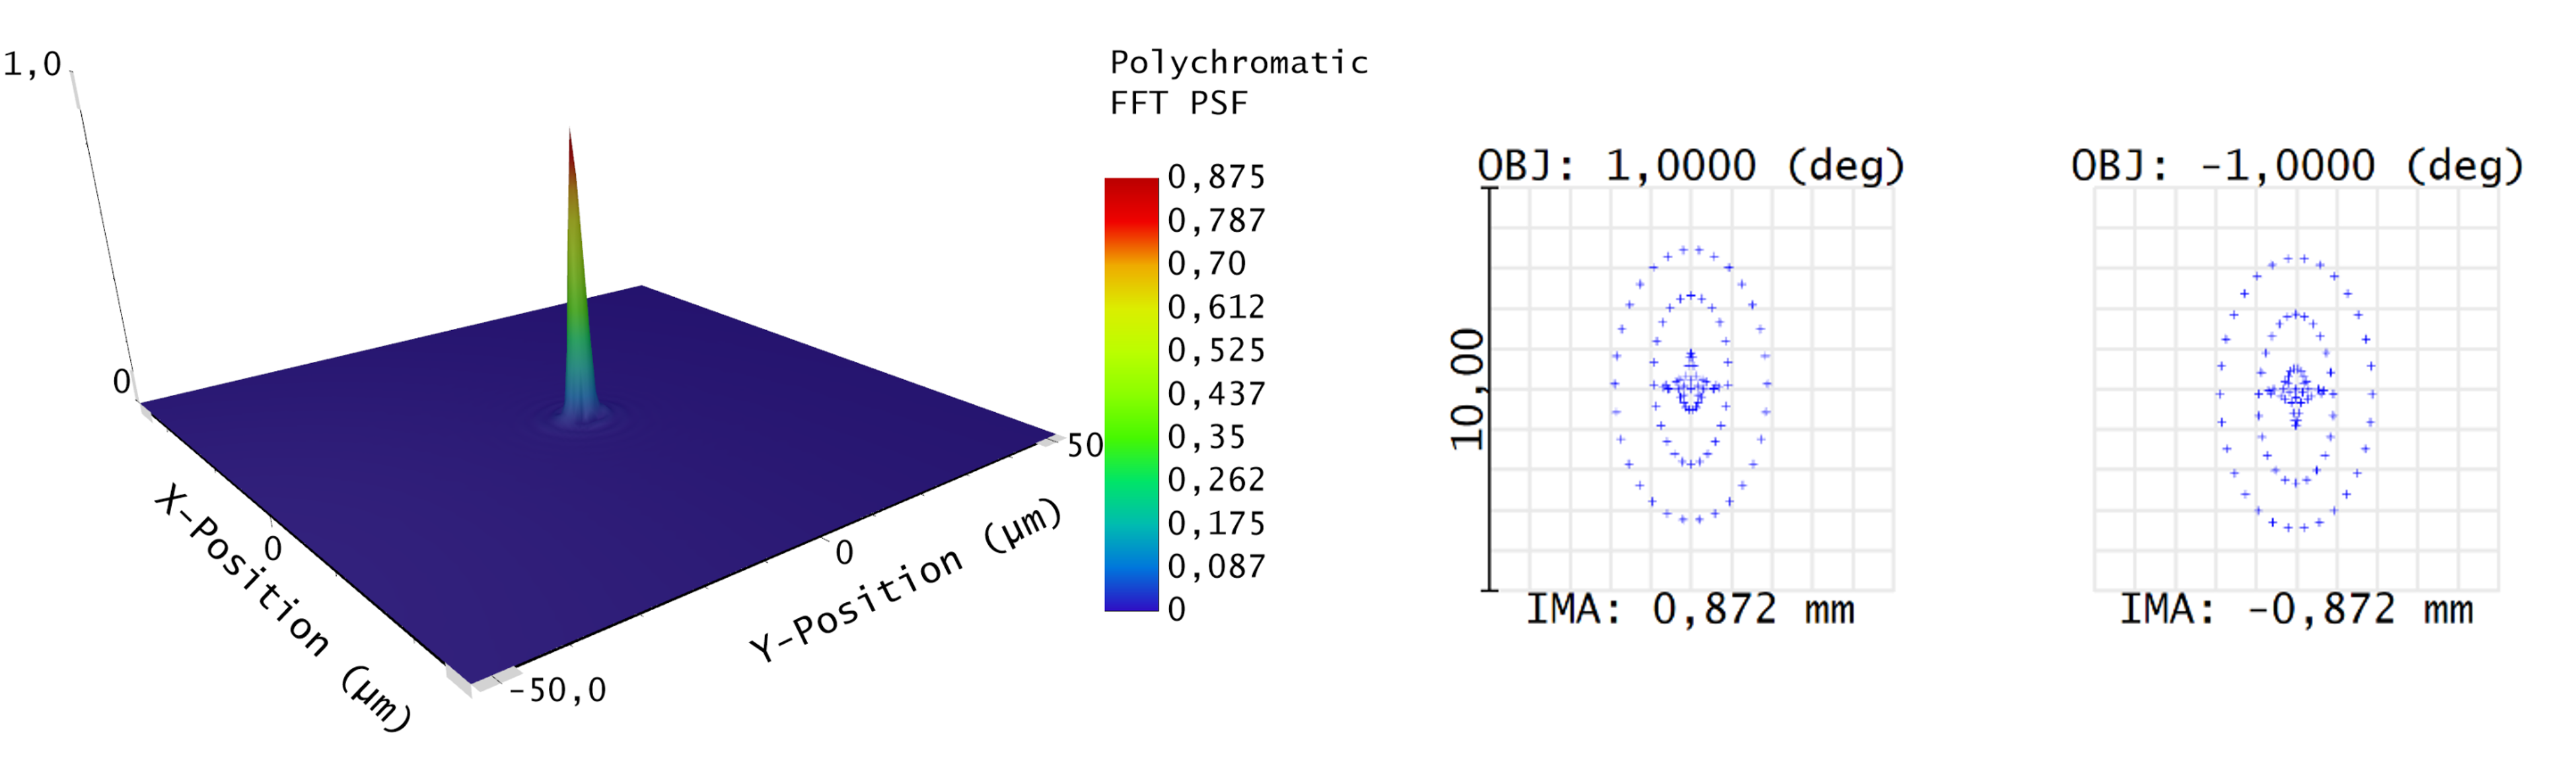
\includegraphics[scale=0.5]{assets/figures/Optical Design/Zemax_PSF.png}
    \caption{PSF and Spot diagram for the chosen lens}
    \label{fig:Opti_ZemaxPSF}
\end{figure}
\subsection{Strehl ratio}
The Strehl ratio compares the peak intensity of the actual focused image to that of an ideal, 
diffraction-limited image formed by a perfect optical system. A Strehl ratio of 1 indicates perfect performance, 
while lower values indicate the presence of aberrations.
\begin{figure}[H]
    \centering
    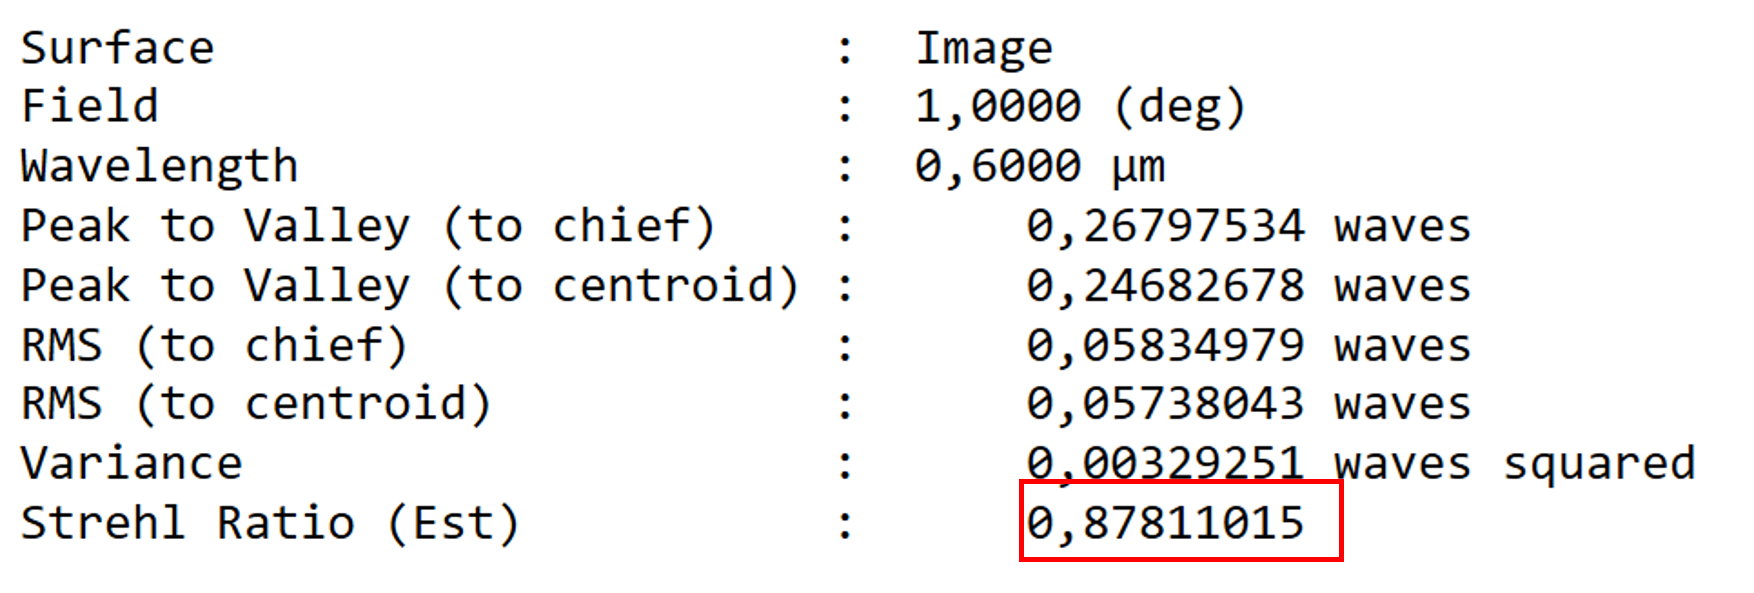
\includegraphics[scale=0.8]{assets/figures/Optical Design/Zemax_Strehl.png}
    \caption{Strehl lens ratio}
    \label{fig:Opti_ZemaxStrehl}
\end{figure}
In this case, the strehl ratio is 0.878. This indicates that the lens, in its configuration, 
has the necessary parameters for this application. \textbf{\textcolor{red}{A finir}}
\newpage
\subsection{Zernik polynomials}
Zernike polynomials define the output wavefront of a system. Each coefficient of this polynomial refers to an
aberration in the optical system. The aim is to minimize these polynomials to obtain, in the best (theoretical)
case, an image that is completely identical to the object. For this project, the polynomials that must be as small as possible are :
\begin{itemize}
    \item \textbf{2-3} : Tilt : The higher this parameter, the greater the tilt on the X and Y axes. Too high a tilt will distort
          the image and sunspot detection may not work.
    \item \textbf{4}   : Defocus : It happens when an optical system fails to converge light rays onto a single point. The higher the
          defocus setting, the greater the contrast between blur and sharpness.
    \item \textbf{5-6} : Astigmatism : This is the most important parameter in this project. Astigmatism compromises image
          sharpness when the beams are far from the optical axis. The appearance of a blur on the final image could compromise the
          measurement. The image would be averaged, in which case the seeing would not be fixed.
    \item \textbf{7-8} : Sphericity : Spherical aberration is an optical aberration that occurs when a lens or mirror fails to focus all
          incoming light rays to a single point. It causes blurring and loss of sharpness in the resulting image. Once again, if the measurement
          is blurred, this will result in a seeing that has not been fixed and therefore an inaccurate measurement.
\end{itemize}
\begin{figure}[H]
    \centering
    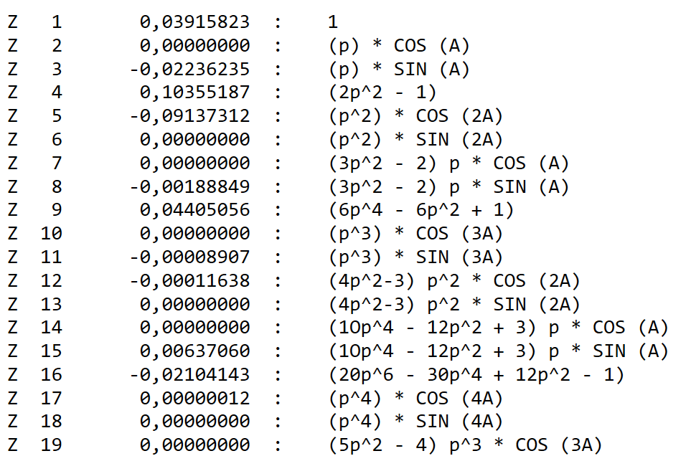
\includegraphics[scale=0.9]{assets/figures/Optical Design/Zemax_Zernik.png}
    \caption{Lens zernik polynomials}
    \label{fig:Opti_ZemaxZernik}
\end{figure}
\textbf{\textcolor{red}{Expliquer pourquoi c'est bien}}
\subsection{Final choice}
\begin{figure}[H]
    \centering
    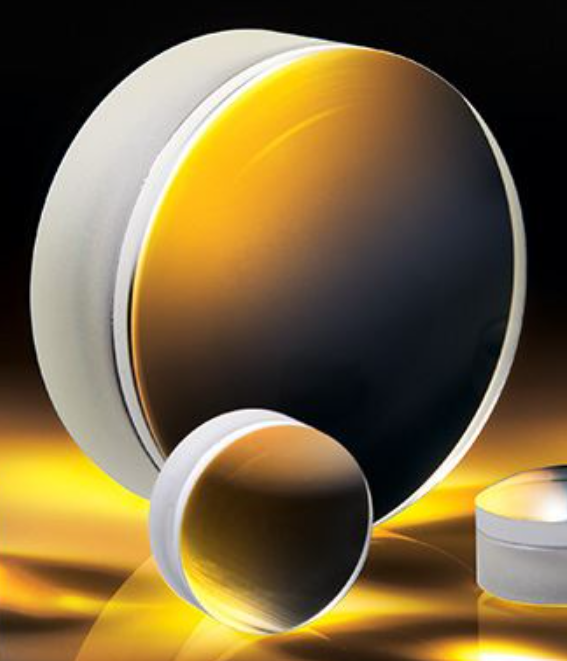
\includegraphics[scale=0.7]{assets/figures/Mechanical Design/Lentille.png}
    \caption{Lens choosed}
    \label{fig:Opti_Lens}
\end{figure}
The lens chosen for the system is the one shown in figure \ref{fig:Opti_Lens}, and was selected in combination with all
the other elements as explained in section \ref{sec:Opti_Limit}. The lens has the following characteristics:
\begin{itemize}
    \item Type: Achromatic Lens
    \item Effective Focal Length EFL (mm): 50.00
    \item Wavelength Range (nm): 425 - 675
    \item Coating Specification: Ravg ≤0.4\% @ 425 - 675nm
\end{itemize}
%====================================================================================================
%====================================================================================================
% Prism selection
%====================================================================================================
%====================================================================================================
\newpage
\section{Prism selection}\label{sec:Opti_Prism}
As far as the prism is concerned, the limiting factor is the beam exit angle. This angle will influence the choice of lens.
\newline
The primary objective was to create a custom-made prism in the shape of a square-based pyramid. This would have made it
possible to produce 4 images and thus refine the measurement. After several requests for bids, it turned out that a custom-made
square-based prism was too expensive ($\approx$ 4000 CHF). After that, it was decided to re-tender with a 2-sided prism, but the price
didn't come down. The final solution was to buy a commercially available prism, produced in large numbers. However, this type of
prism is only available in circular format. We therefore had to find a way of adapting and mounting it (Section \ref{sec:prisms}).
\bigbreak
The search for prisms was therefore carried out on the Edmund optics website.
This supplier offers a wide range of prisms with treatments equivalent to the lens treatment.
Available prisms offer beam exit angles ranging from 0.5$^{\circ}$ to 15$^{\circ}$.
\newline
As stated in section \ref{sec:Opti_Lens}, the prism must produce an angle of 1$^{\circ}$ at its exit to correpsond with the
choice of lens. The prism shown in figure 2 was therefore chosen.
\begin{figure}[H]
    \centering
    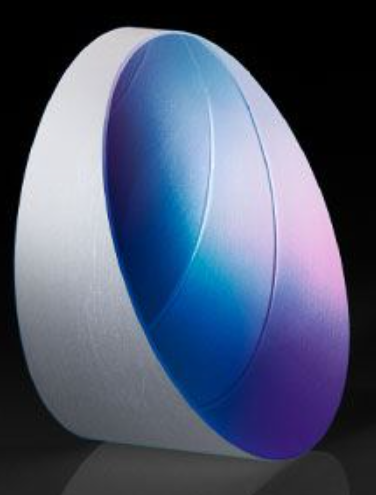
\includegraphics[scale=0.8]{assets/figures/Mechanical Design/Prisme_obtenu.png}
    \caption{Prism choosed}
    \label{fig:Opti_Prism}
\end{figure}
The prism chosen has the following characteristics:
\begin{itemize}
    \item Wavelength Range (nm): 425 - 675
    \item Surface Flatness (P-V): λ/10
    \item Ray Deviation @ 633nm ($^{\circ}$): 1.00
    \item Substrate: N-BK7
    \item Wedge Angle: 1$^{\circ}$ 56'
\end{itemize}
%====================================================================================================
%====================================================================================================
% Limitation
%====================================================================================================
%====================================================================================================
\newpage
\section{Limitations of the system}\label{sec:Opti_Limit}
Parler du ratio du masque etc \newline
Parler du filtre solaire pour le télescope

\begin{figure}[H]
    \centering
    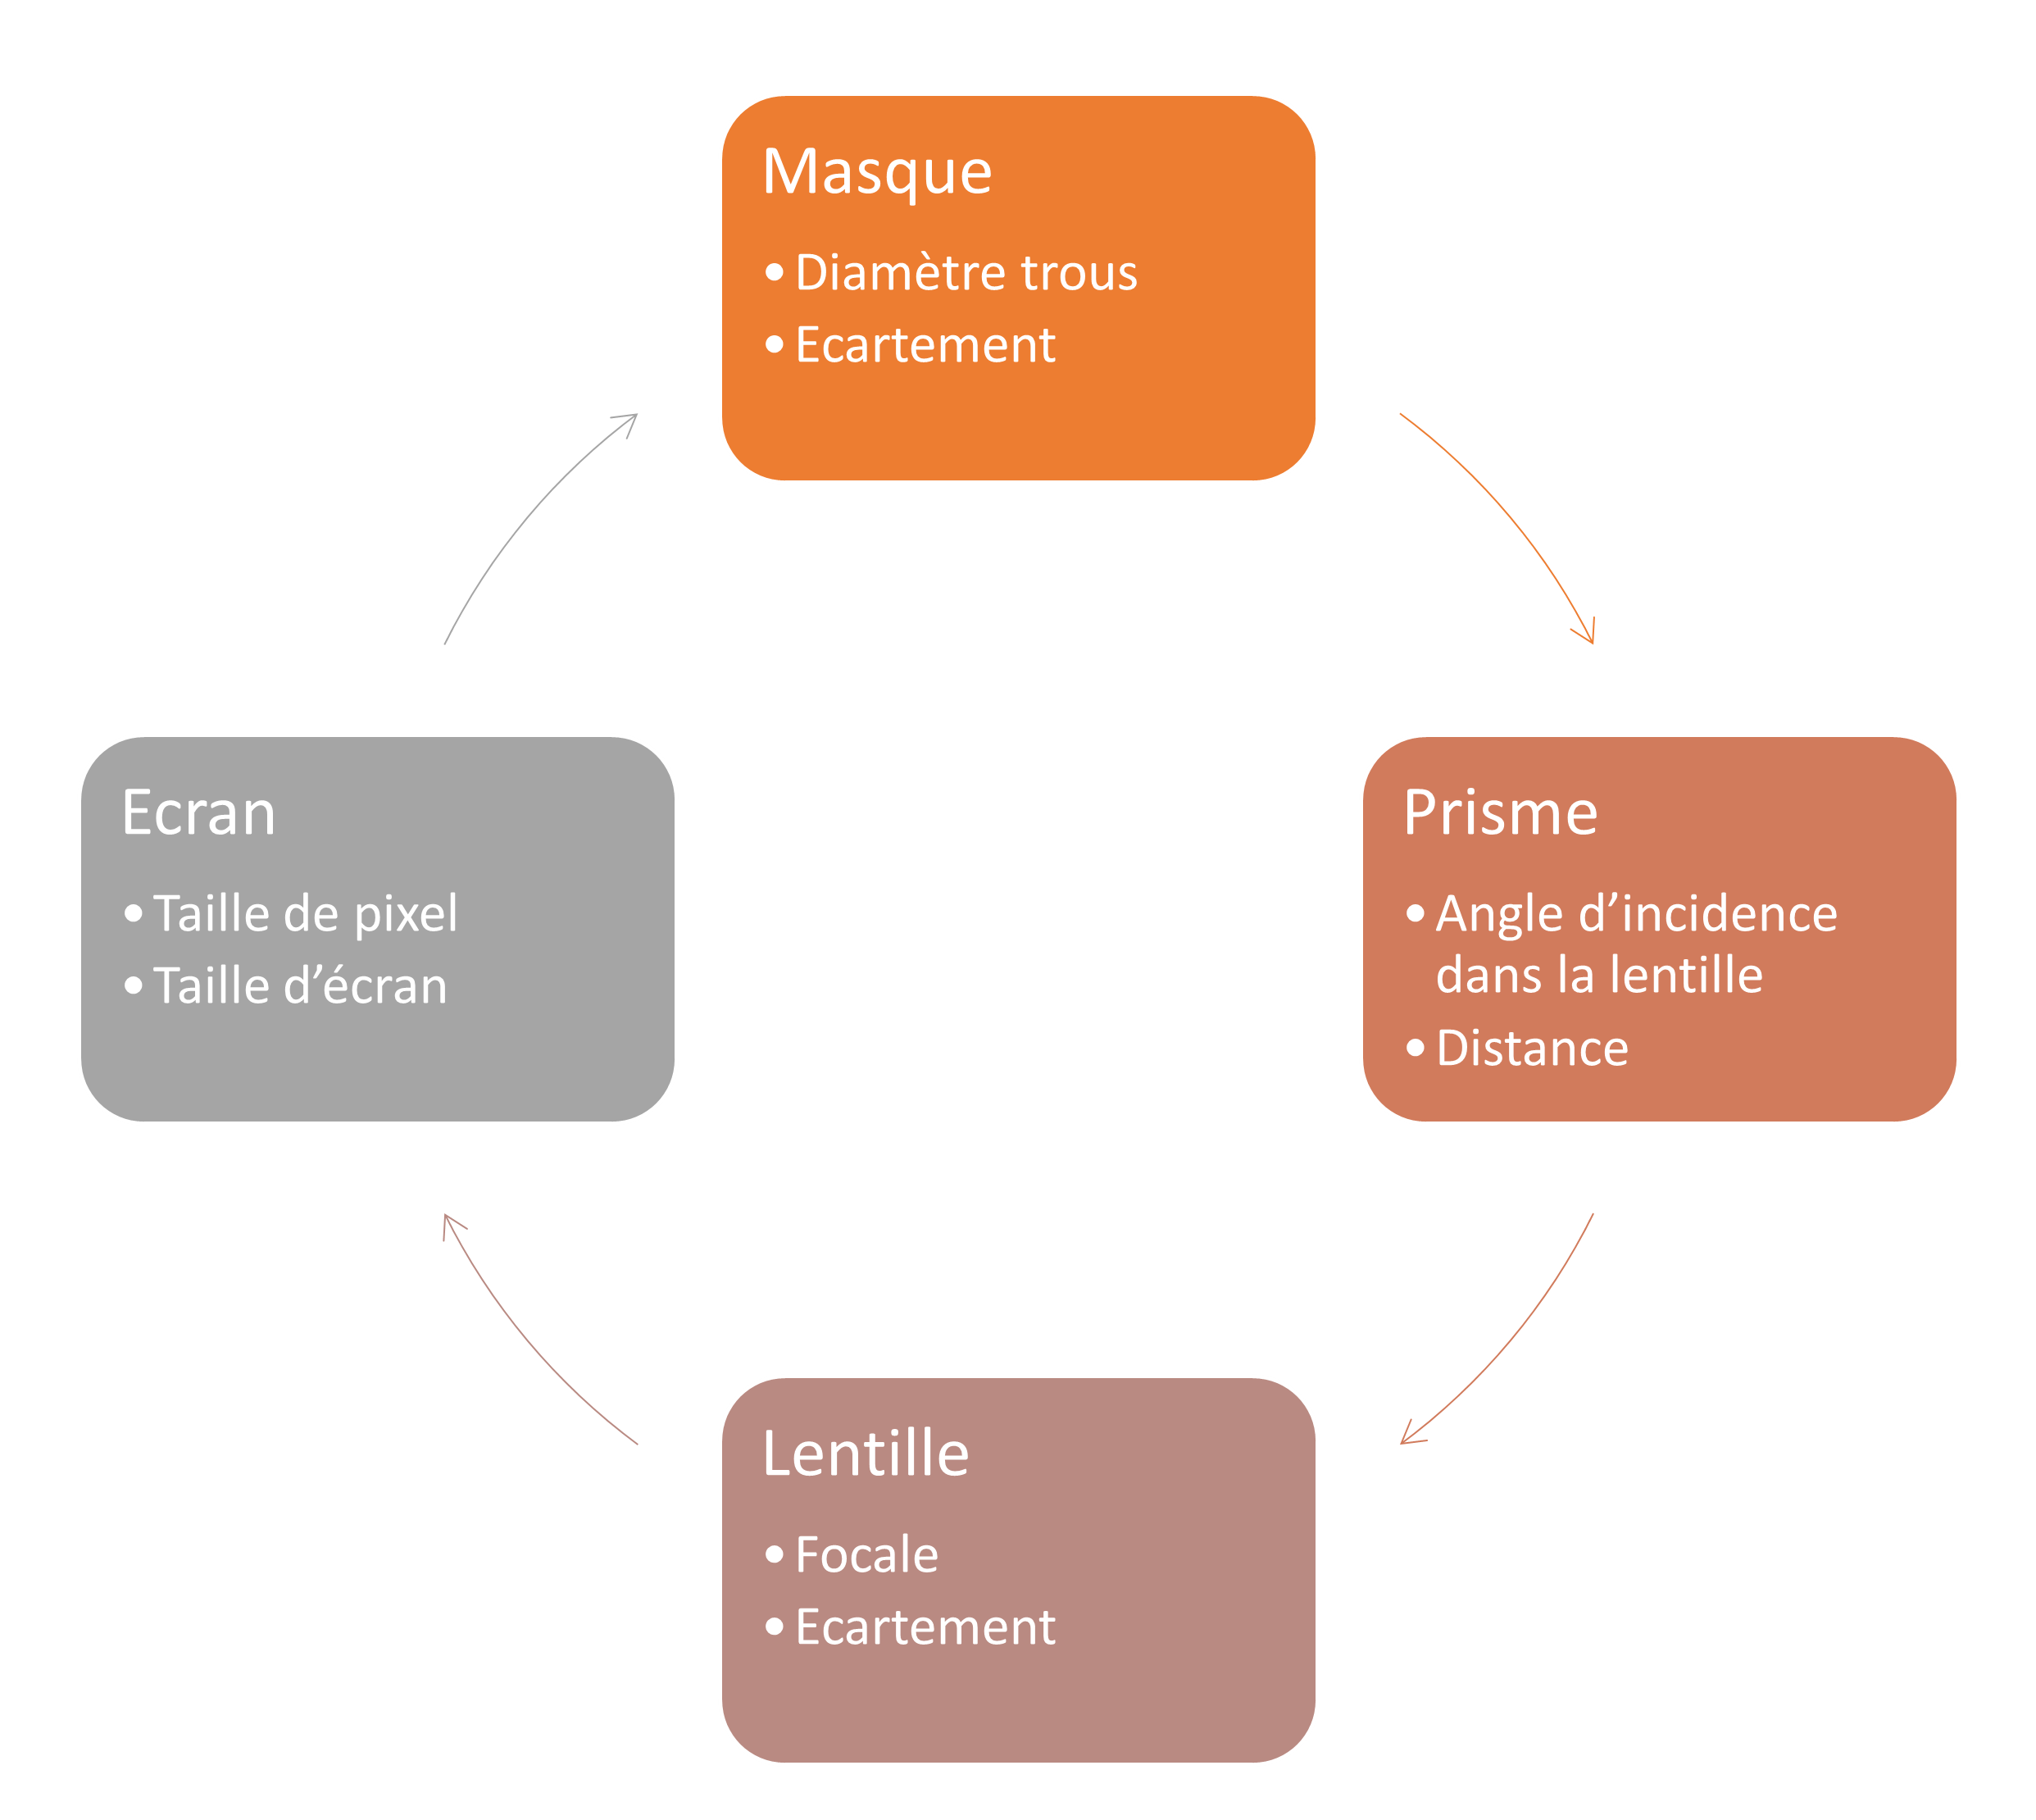
\includegraphics[scale=0.25]{assets/figures/Optical Design/Diagramme_Limitation.png}
    \caption{Component selection diagram}
    \label{fig:Opti_DiagrammChoices}
\end{figure}

\chapter{Mechanical design}
%====================================================================================================
% En-tête
%====================================================================================================
\begin{figure}[H]
    \centering
    \includegraphics[scale=0.65]{assets/figures/Mechanical Design/Système.png}
    \caption{Representation of the Mechanical design}
    \label{fig:Mec_Blobal}
\end{figure}
\newpage
%====================================================================================================
% Preliminary choices and limitations
%====================================================================================================
\section{Preliminary choices and limitations}
\subsection{Objectives}
First, the mechanical system need to be attached to the output of the laboratory telescope. To achieve this, an adaptor piece is
required (\ref{sec:adaptator}). Then, the masks will need to be attached to a support (\ref{sec:mask}). A second support will have
to be made to accommodate the prisms (\ref{sec:prisms}). Finally, the lens must be installed (\ref{sec:lens}) and the camera placed
just behind it (\ref{sec:Camera}). \newline
The system must be compact, adjustable and adaptable if modifications are required at a later date.
\subsection{Limitations}
To make this system a reality, a simple and common fastening system had to be integrated. The most simple system used in optical design 
is the cage system. Two of the world's leading optomechanics manufacturers offer it (Thorlabs and Edmund Optics). The significant difference 
between these 2 manufacturers is the spacing between the steel bars. This difference is shown in the capter \ref{sec:lens}. \newline
To integrate the telescope's occular correctly, the Edmund optics system is required. This is because the distance between the steel bars 
is smaller on the thorlabs system, and the distance between the occular and the bore for the bar would be far too small ($\approx$ 0.05mm).
\bigbreak
The difference between the Thorlabs system and the Edmund Optics system is the centering diameters for the steel bar holes who 
can be seen on the figure \ref{fig:thorlabs_Edmund} ($\emptyset\ 38\ mm$ for Thorlabs (blue) and $\emptyset\ 57\ mm$ for Edmund optics (red))
\begin{figure}[H]
    \centering
    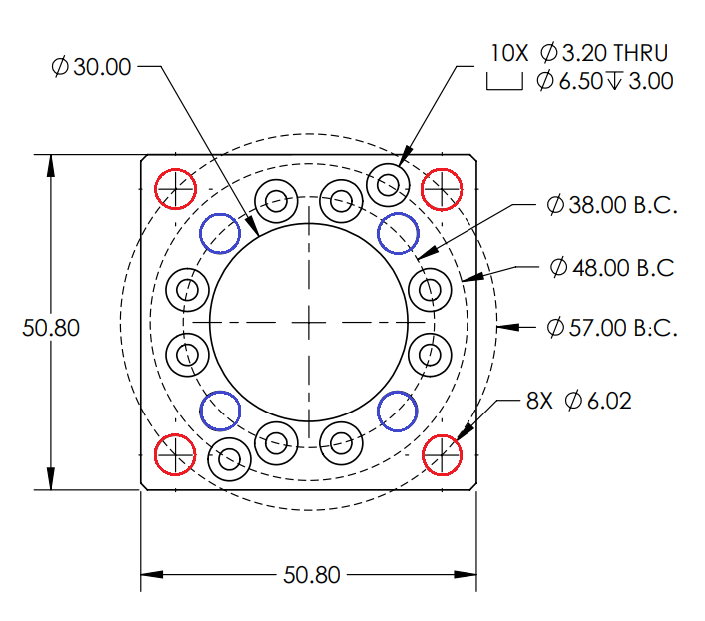
\includegraphics[scale=1]{assets/figures/Mechanical Design/Thorlabs_Edmund.png}
    \caption{Differences between thorlabs and Edmund systems}
    \label{fig:thorlabs_Edmund}
\end{figure}
%====================================================================================================
% Telescope mounting system
%====================================================================================================
\section{Telescope mounting system}\label{sec:adaptator}
The telescope-mounting system, as its name suggests, will be the connecting piece between the telescope output and the \Gls{DIMM}. It will 
also integrate the telescope's occular. The choice of integrating the telescope's ocular with this part was made to improve the system's 
stability and alignment. The system will be screwed onto the telescope, so it won't be held in place by simple screws attached to 
the part. \newline
This part will maintain all the \Gls{DIMM}. So it need to be strong and more massive than the other parts. However, it also needs to be as 
light as possible so as not to weigh too much on the telescope. Material was therefore removed from the middle of the piece to reduce 
its weight.
\bigbreak
Figure \ref{fig:Mec_Adapter1} (Adapter drawing) shows :
\begin{enumerate}
    \item The hole for the ocular ($\emptyset\ 33.55\ mm$) and the thread for its attachment ($MF\ 40\ P=1$). Fixing is simply done 
    with a threaded ring drilled through the center.
    \item The thread for attaching the system to the telescope ($\emptyset\ 50.75\ mm\ TPI\ 24$)
    \item Hole for steel bars and the screws used to secure them ($\emptyset\ 6.02$)
\end{enumerate}
\begin{figure}[H]
    \centering
    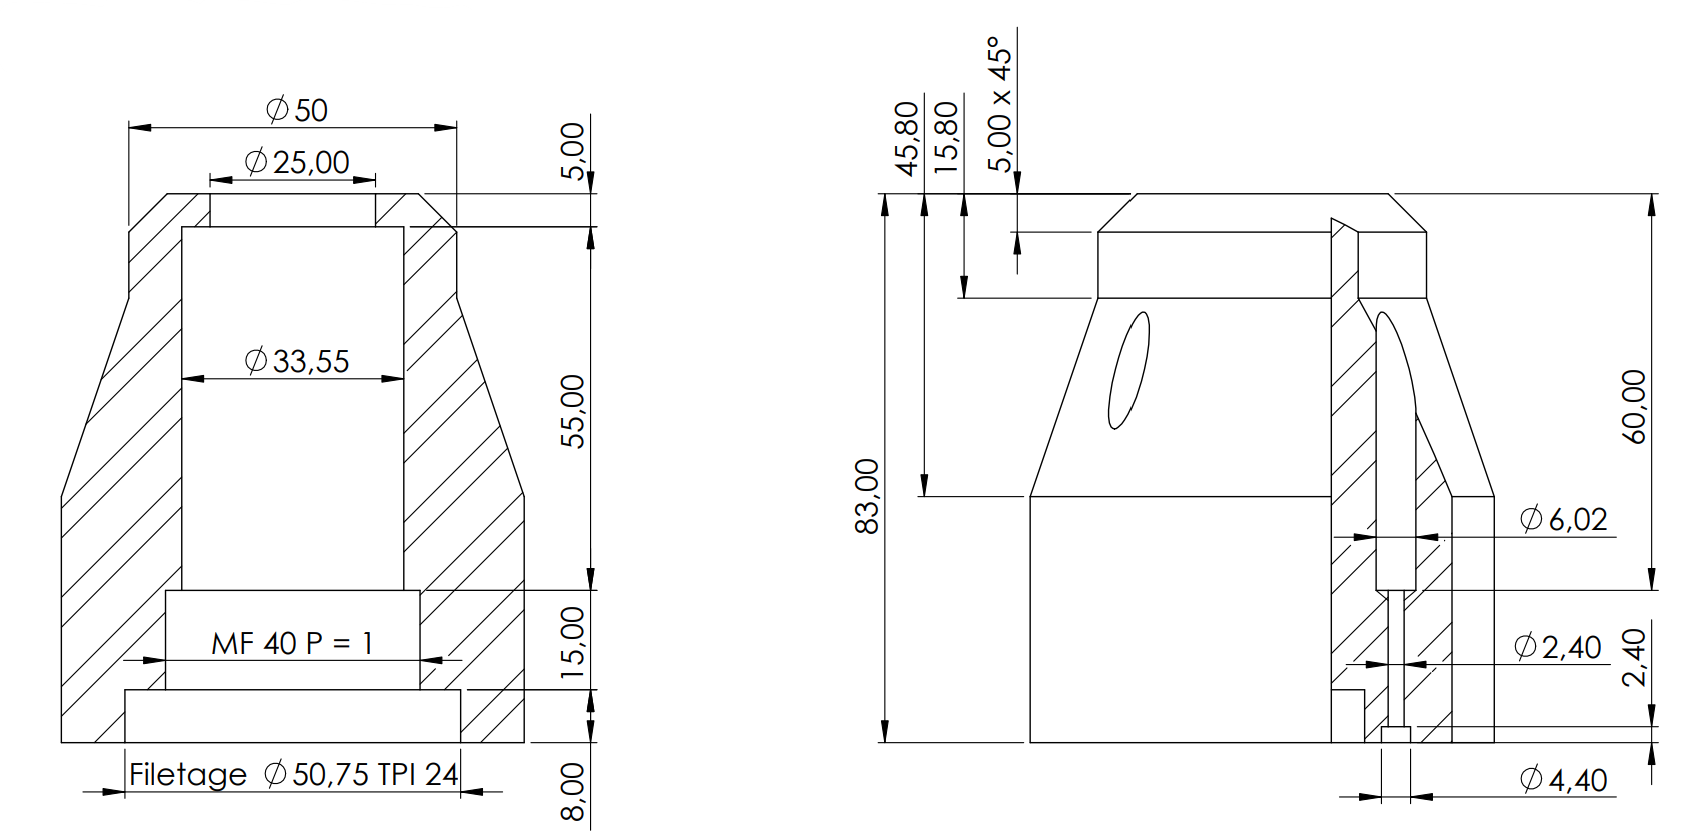
\includegraphics[scale=0.6]{assets/figures/Mechanical Design/Dessin_Part1_adapter.png}
    \caption{Representation of the adaptator : ocular and bar fixation}
    \label{fig:Mec_Adapter1}
\end{figure}
This part will be made of aluminum to reduce its weight. The use of aluminum has no effect on the rigidity of the system. \newline
However, the ocular attachment ring will be made of steel to limit the coefficient of friction when screwing it on 
(screwing an aluminum part with another of this material will have a grip effect between the two parts).
\bigbreak
The complete drawing can be found in the appendix \ref{App:MEP}
\newpage
%====================================================================================================
% Mask mounting
%====================================================================================================
\section{Mask and mounting}\label{sec:mask}
\subsection{Mask}
As explained in section \ref{sec:Opti_Limit}, the mask will have 2 holes 1mm in diameter, with their centers 5mm apart. 
A 0.5mm-thick plate was designed for this purpose. This plate includes the 2 holes and is shaped to fit more easily into its support.
This part is shown in figure \ref{fig:Mec_Mask}
\begin{figure}[H]
    \centering
    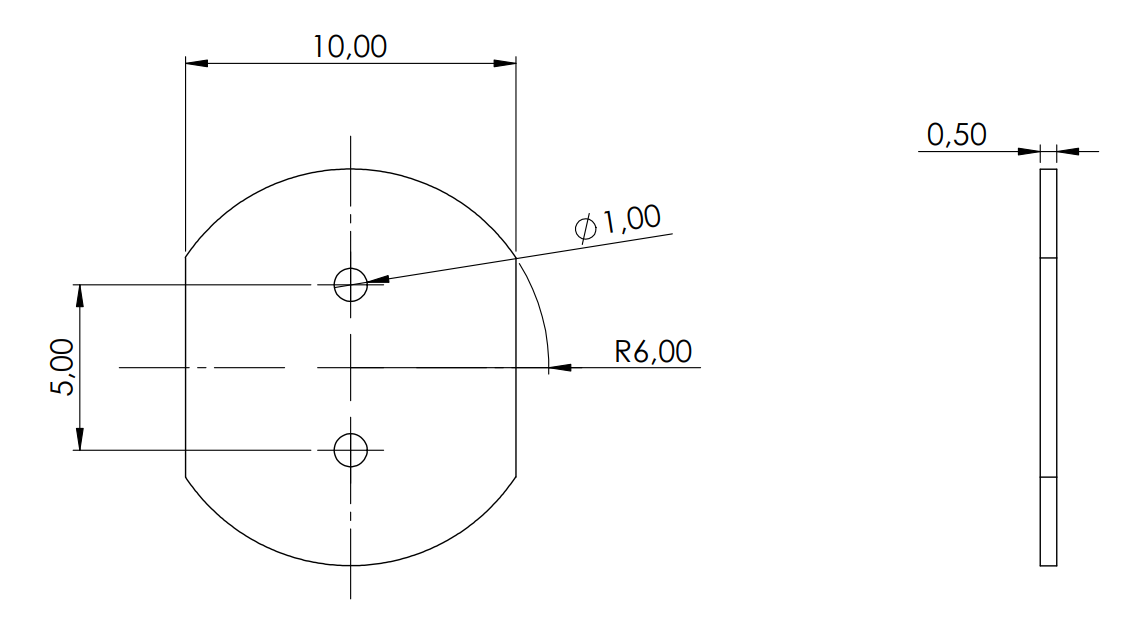
\includegraphics[scale=0.55]{assets/figures/Mechanical Design/Dessin_Mask.png}
    \caption{Drawing of the mask}
    \label{fig:Mec_Mask}
\end{figure}
\subsection{Mounting}
For the support, 2 pieces are required. The first will contain the "rail" where the mask will be inserted (Figure \ref{fig:Mec_Mask_Sup_Rail} left),
 and the other will hold it in place (Figure \ref{fig:Mec_Mask_Sup_Rail} right).
\begin{figure}[H]
    \centering
    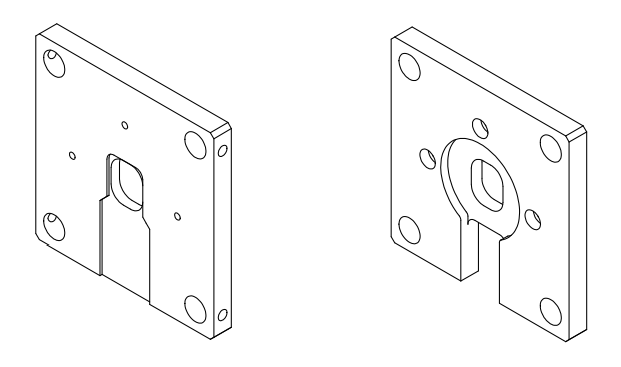
\includegraphics[scale=0.85]{assets/figures/Mechanical Design/Support_masque_rail.png}
    \caption{Supports for the mask}
    \label{fig:Mec_Mask_Sup_Rail}
\end{figure}
Figure \ref{fig:Mec_Mask_Sup_Rail} (left) shows the mask positioning rail, the tapped holes for attaching the second part and the holes 
for the steel bars. \newline
Figure \ref{fig:Mec_Mask_Sup_Rail} (right) shows the second piece who is designed for easy mask removal. This part also features the opening 
for inserting the mask, as well as the screw holes for securing the two parts together.\bigbreak
This part will be made of aluminum to reduce its weight. The use of aluminum has no effect on the rigidity of the system.
\bigbreak
The complete drawing can be found in the appendix \ref{App:MEP}
%====================================================================================================
% Prisms and mounting
%====================================================================================================
\section{Prisms and mounting}\label{sec:prisms}
\subsection{Prisms}
As explained in section \ref{sec:Opti_Prism}, the output beams from the prism must have an angle of incidence of 1°. 
This corresponds to an angle of 1.93° on the prism. \newline
Several requests for bids were made, but none were within the budget allocated under the TB. The aim was to have a square-shaped 
prism (\ref{fig:Prism_square} left) to reduce the size of the system and make it easier to assemble. However, this solution could not be retained and the 
use of circular prisms (\ref{fig:Prism_square} right) was required. This solution greatly reduces the budget, but the part that will hold them will be much more complex.
\begin{figure}[H]
    \centering
    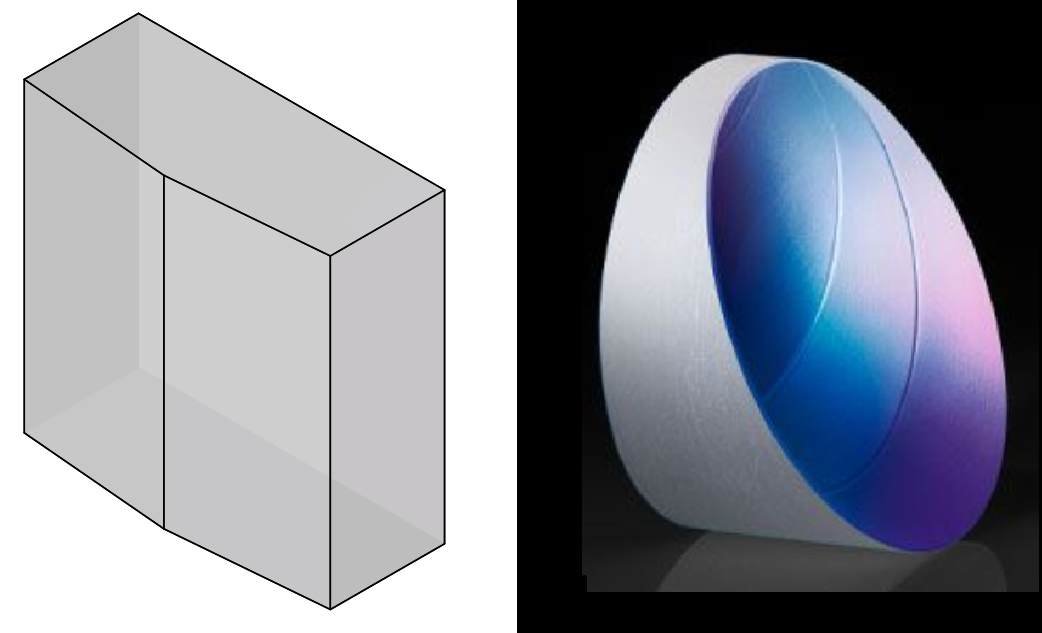
\includegraphics[scale=0.5]{assets/figures/Mechanical Design/prisme_voulu.png}
    \caption{Needed prism / Prism choosed}
    \label{fig:Prism_square}
\end{figure}
\subsection{Mounting}
To attach the 2 prisms, we had to create a custom-made part. To achieve this, several elements were critical 
like direction, position and orientation of the prism.
\bigbreak
For these purpose, a maintenance part has been created (Figure \ref{fig:Prism_Support1}). This part will allow the 2 prisms to be inserted, while letting 
the beam from the mask pass through. \newline
There are 2 small notches on the back of the part. These notches are there to ensure correct mounting of the prism's 
holding parts (Figure \ref{fig:Prism_Support2}).\newline
This part also has holes and threads for fixing the assembly to the steel bars, and for attaching the part that 
will hold the prisms in position. 
\begin{figure}[H]
    \centering
    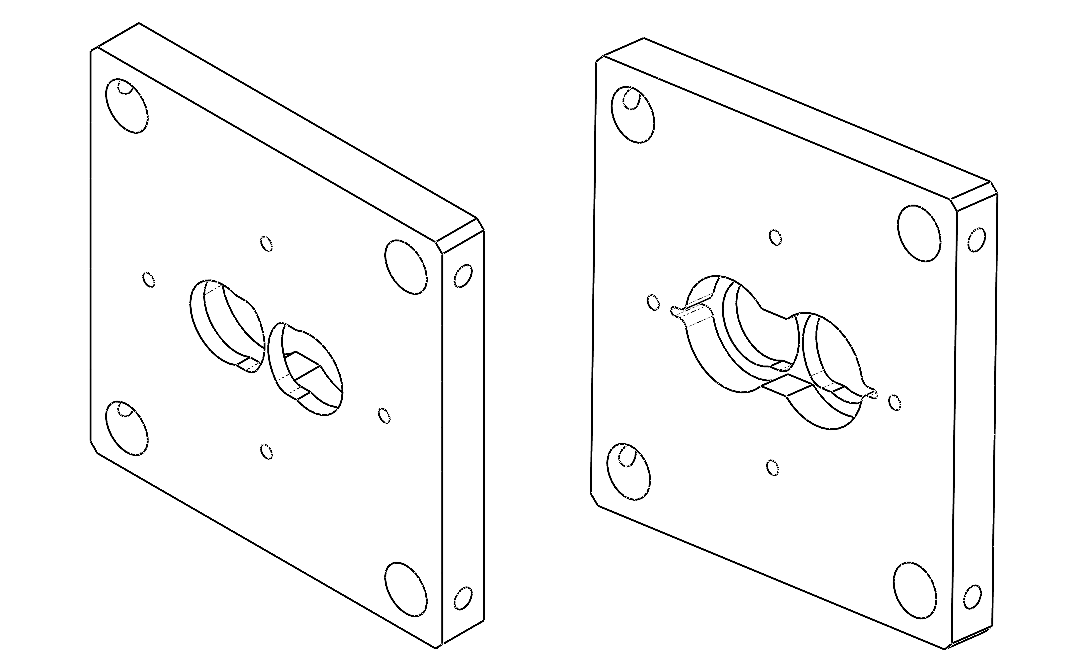
\includegraphics[scale=0.55]{assets/figures/Mechanical Design/MaintientPrism1.png}
    \caption{Support for the prisms}
    \label{fig:Prism_Support1}
\end{figure}
The part shown in figure \ref{fig:Prism_Support2} was created to fix and hold the prisms correctly. This part fits perfectly into the support 
bore and will be positioned with the notches. \newline 
This part is made with the same angle of inclination as the prisms on one side, so as to be able to fix them perfectly. 
If the prism is not correctly positioned, the part will protrude more strongly from its support. If the prism is in its 
deepest position, it will be correctly mounted and the clamp can be installed.\newline
During assembly, this part requires particular attention. They must be handled with care to avoid damaging the prisms.
\begin{figure}[H]
    \centering
    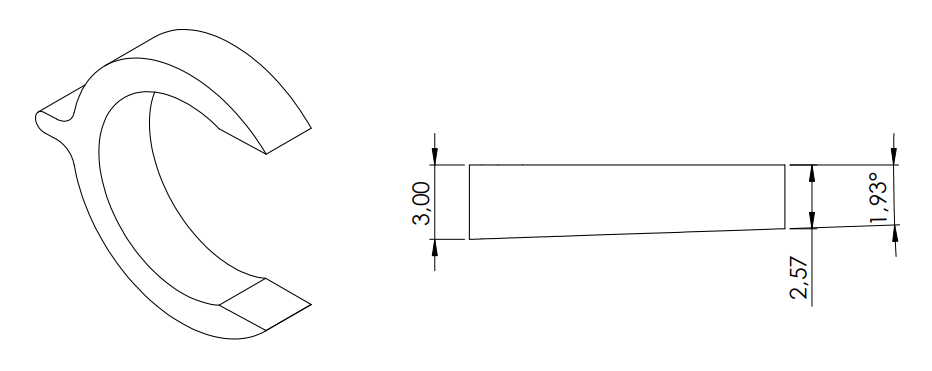
\includegraphics[scale=0.7]{assets/figures/Mechanical Design/MaintientPrism2.png}
    \caption{Prism wedge}
    \label{fig:Prism_Support2}
\end{figure}
The last piece will be used to hold the assembly in position (Figure \ref{fig:Prism_Support3}). It rests on the prism wedges 
and is attached to the support piece (Figure \ref{fig:Prism_Support1}). \newline
During assembly, this part requires particular attention. When tightening the parts, you'll need to tighten each screw a 
little at a time, so that the part remains as parallel as possible to the support.
\begin{figure}[H]
    \centering
    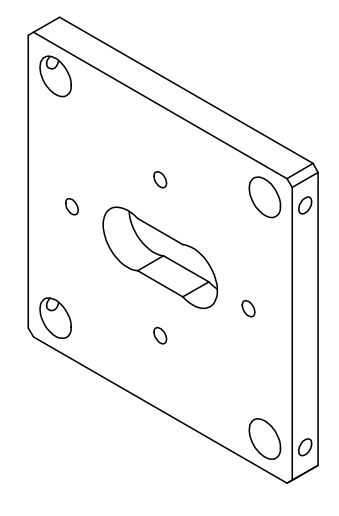
\includegraphics[scale=0.8]{assets/figures/Mechanical Design/MaintientPrism3.png}
    \caption{Clamp for prism support}
    \label{fig:Prism_Support3}
\end{figure}
All these parts will be made of aluminum to reduce its weight. The use of aluminum has no effect on the rigidity of the system.
\bigbreak
The complete drawing can be found in the appendix \ref{App:MEP} for the support and \ref{App:Edmund_MEP} for prisms
%====================================================================================================
% Lens and mounting
%====================================================================================================
\section{Lens and mounting}\label{sec:lens}
\subsection{Lens}
As explained in section \ref{sec:Opti_Limit}, the lens need to be achromatic with a spectrum from 425nm to 675nm 
and a focal lenght of 50mm. For mechanical reasons (size of supports), a 25mm diameter lens had to be integrated. 
\begin{figure}[H]
    \centering
    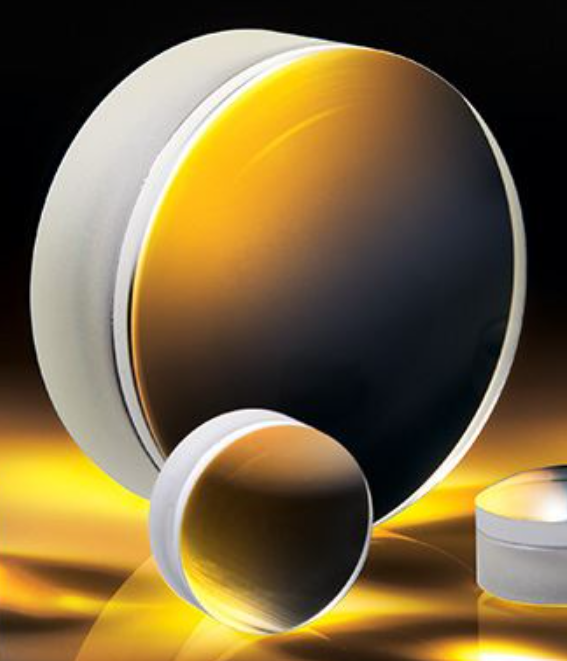
\includegraphics[scale=0.65]{assets/figures/Mechanical Design/Lentille.png}
    \caption{Achromatic lens F = 50mm (425nm - 675nm)}
    \label{fig:Lentille}
\end{figure}
\subsection{Mounting}
This part of the mechanics is much simpler because everything has been ordered from the Edmund optics website. 
The mechanics used to hold the lens in place are a support that attaches to the steel bars, and a cage for 
the lens that attaches directly to the support.
\begin{figure}[H]
    \centering
    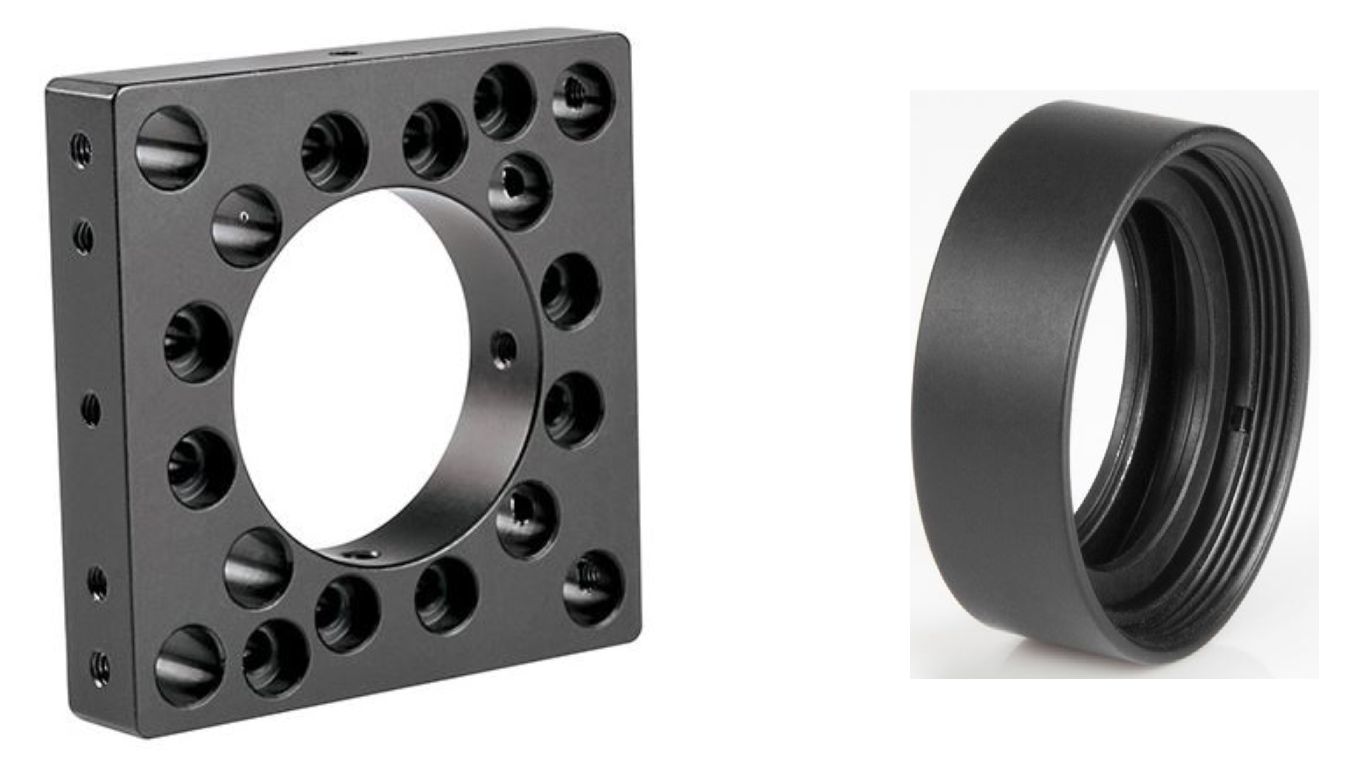
\includegraphics[scale=0.55]{assets/figures/Mechanical Design/Support_Lentille.png}
    \caption{Support and cage for the lens}
    \label{fig:Lentille_Support1}
\end{figure}
\bigbreak
The complete drawing can be found in the appendix \ref{App:Edmund_MEP}
\newpage
%====================================================================================================
% Camera mounting
%====================================================================================================
\section{Camera mounting}\label{sec:Camera}
\subsection{Camera}
As explained in section \ref{sec:Opti_Cam}, the chosen camera is Allied Vision's Alvium 1800 U-052m. \newline
It can be mounted on the front panel using either the C-mount thread or four tapped 
holes. It is also possible to attach to these sides with four additional threaded holes.
\begin{figure}[H]
    \centering
    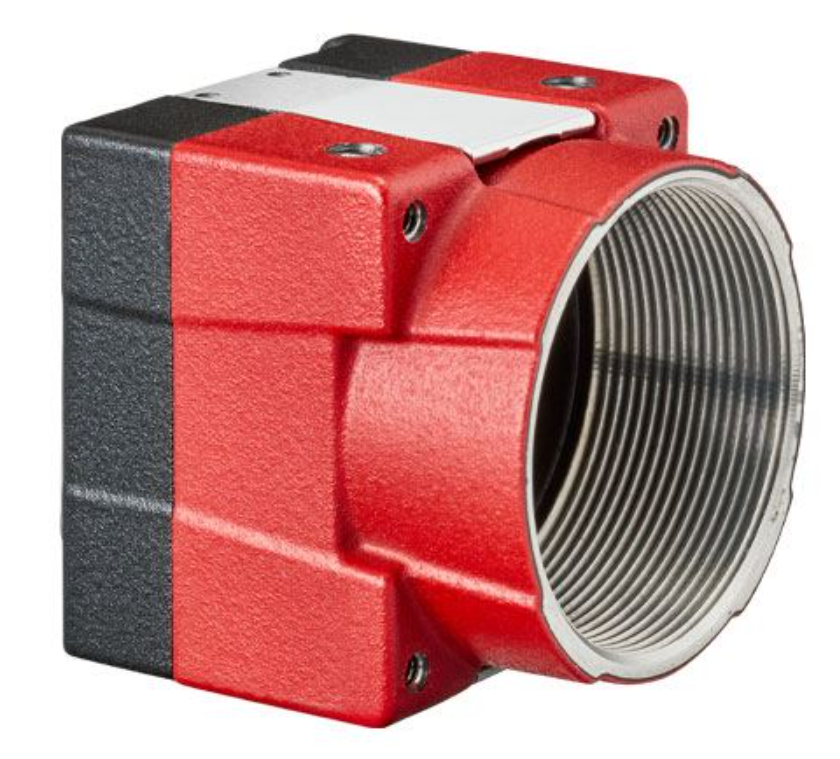
\includegraphics[scale=0.35]{assets/figures/Mechanical Design/Camera.png}
    \caption{Selected camera}
    \label{fig:Camera}
\end{figure}
It was decided to attach the camera via its C-mount thread. After receiving the camera, it was noted that the 
optimum operating temperature for the electronics was 85°C, which causes the casing to heat up considerably. 
It might be necessary to add coolers (or even a fan) at a later date if the tests are not conclusive. 
Other threaded holes could be used to cool the system (cooler attachment).
\subsection{Mounting}
For the camera, a bracket will be designed to hold it in position. The housing has a threading system 
(C-mount) that is very common in the optical world. This is a mounting used for lenses that can be added 
to this type of camera. The part shown in figure \ref{fig:Camera_Support} corresponds to the bracket and comprises 
an external C-mount thread around the shoulder and holes for steel bars.
\break
The camera will be screwed onto the bracket. Its orientation will pose no problem, as the images of our 
stars/sunspots will always be in the sensor area. However, the software will have to be designed to find 
the areas of interest easily and efficiently.
\begin{figure}[H]
    \centering
    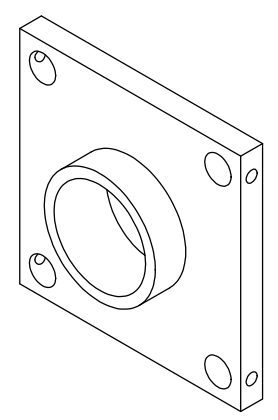
\includegraphics[scale=0.75]{assets/figures/Mechanical Design/Support_Camera.png}
    \caption{Support for the camera}
    \label{fig:Camera_Support}
\end{figure}
\bigbreak
The complete drawing of the support can be found in the appendix \ref{App:MEP} and the drawing of the camera 
in the appendix \ref{App:Edmund_MEP}.

\chapter{Software}
%====================================================================================================
% Possibilities and choices
%====================================================================================================
\section{Possibilities and choices}
\subsection{Possibilities}
\subsubsection{measurement method}
Two options are available for creating the software:
\begin{enumerate}
    \item \textbf{Pre-capture of images using Vimba software (\ref{sec:Vimba})} : \newline
          In this case, the images are taken using the software supplied with the camera and then entered into the software develop with python.
          The problem is that the operator carrying out the measurement will have to switch between initialization parameters and parameters
          for measurements on the Vimba software. For this solution, different software modes will also be required
    \item \textbf{Image capture and analysis} :\newline
          The second solution involves automatic measurement and initialization. The operator would simply point the telescope at an
          object and launch the software. The problem with this solution is that it would be more complex to detect a bug. In this case,
          we'd have to come up with solutions to recognize measurement bugs as quickly as possible.
\end{enumerate}
\subsubsection{Initialization}
For initialization, two solutions are also possible :
\begin{enumerate}
    \item The first is to take several images with a exposure time equal to the measurement part. By adding up all the images,
          the turbulence will be averaged. It will then be easy to determine the object's center of gravity and its centroid.
    \item The second option would be to considerably increase the exposure time of the image. This would be the same as the
          previous option, but taking only 1 image would reduce memory usage and increase computing speed.
\end{enumerate}
In these 2 cases, the number of images to be used or the exposure time required to correctly average the image will need to
be determined during the initial tests. If turbulence is not properly averaged, aberrant results may appear.
\subsection{Choices}
\subsubsection{measurement method}
The software will feature both methods of use. However, the pre-capture method with Vimba software will not yet be implemented in its first version.
The addition of this possibility could be agreed at a later date if there is a real interest.
\subsubsection{Initialization}
The chosen initialization method is to take several images with minimal pause time. \newline
Using a longer pause time could result in unwanted elements appearing in the image.
What's more, the images used during initialization could be reused for measurement. The basic principle of initialization is :
\begin{itemize}
    \item Take \textit{X} images to average turbulence.
    \item Recognition of centers of interest.
    \item Localization of image centers.
    \item Recovering the size of the centers of interest for cropping during measurement.
\end{itemize}
The number of images to be taken for the centroid to be as accurate as possible will be determined during testing.
If the disturbance is measured on a star, it is possible to take images in an automated way until the average image
is as circular as possible (the star would have been deviated at any point internal to the turbulence).
\subsubsection{Measurement}
The measurement program will be simple in principle. However, when image processing is involved in a process, the main issue is reliability.
The measurement program must :
\begin{itemize}
    \item Take a shot with the shortest possible exposure time.
    \item Image adjustment.
    \item Find the 2 points of interest in the image.
    \item Determine their centroid.
    \item Recover the result of the difference with the initialization centroid.
    \item Repeat the above points several times.
    \item Calculate the variance of centroid deviations
    \item Transform value into Fried parameter
\end{itemize}
As stated at the beginning of this section, image processing is a very sensitive element in the program. To achieve this,
multiple tests will have to be carried out in order to certify the robustness of its use.
%====================================================================================================
% Vimba software
%====================================================================================================
\newpage
\section{Vimba software}\label{sec:Vimba}
The Vimba software package was created by Allied Vision and is available to all users of Allied Vision cameras.
The software lets you modify camera parameters in real time (Figure \ref{fig:Soft_Vimba}). It is also designed to pre-process
the image before sending it for output. Inputs are also available to control the camera.
\begin{figure}[H]
    \centering
    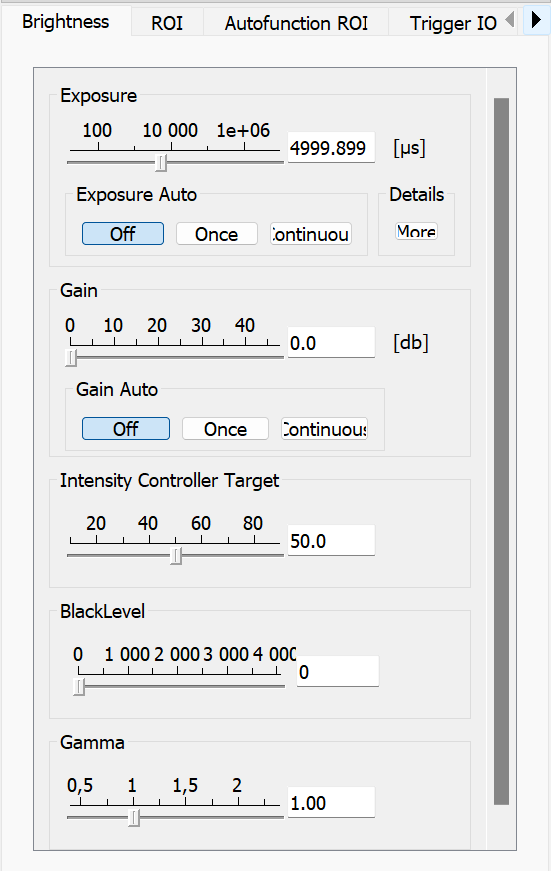
\includegraphics[scale=0.85]{assets/figures/Software/VimbaInterface.png}
    \caption{Editable image parameters on Vimba}
    \label{fig:Soft_Vimba}
\end{figure}
This application is very useful for adjusting parameters during measurements, but also for initial tests, as several images can
be taken in quick succession using one of the software's functions (With the "Image series options" parameter).
%====================================================================================================
% Python API for Vimba
%====================================================================================================
\newpage
\section{Python API for Vimba}
The Vimba software introduced in section \ref{sec:Vimba} is also supplied with an API for simulating the software on python.
All API data is given in a git directory (\href{https://github.com/alliedvision/VimbaPython}{Github link}) and the user manual
can be found in appendix \ref{App:pythonVimba}.\newline
Please note that if the Vimba program is open on the computer, the API will not be able to communicate with the camera.
\subsection{Camera connection}\label{sec:Soft_API_Connect}
Before using the camera with the API, the code must call the procedure that simulates the Vimba program :
\begin{verbatim}
    with Vimba.get_instance() as vimba:
        cams = vimba.get_all_cameras()
        with cams[0] as cam:
            // Your code
\end{verbatim}
In the code above, the "cam" structure is the element to be called in order to access all the camera parameters.
With this structure, image parameters, setups and access to images can be carried out.
\subsection{Parameter modification}
The API also lets you change camera parameters separately. In the case of the \Gls{DIMM} application, the most important
need is to change the exposure time. To do this, once the camera is connected (Code in section \ref{sec:Soft_API_Connect}),
call this function:
\begin{verbatim}
    exposure_time.set(2000) #us
\end{verbatim}
This function lets you change the exposure time (given in microseconds) and can range from 20 to 10000000 (10 seconds).
\subsection{Load and save settings}
\subsubsection{Save settings}
Pre-recorded settings files can be created for the camera. If certain values are modified and you wish to keep them,
you can save the file on your computer. To do this, after connecting to the camera (\ref{sec:Soft_API_Connect}),
simply call up the function :
\begin{verbatim}
    settings_file = 'my_File.xml'
    cam.save_settings(settings_file, PersistType.All)
\end{verbatim}
\subsubsection{Load settings}
To retrieve settings that have already been saved and load them into the camera, use the code below:
\begin{verbatim}
    settings_file = 'my_File.xml'
    cam.load_settings(settings_file, PersistType.All)
\end{verbatim}
\newpage
\subsection{Image capture}
Before taking an image, you need to be able to set a format compatible with the compiler or
a library that will be used to create the software. To do this, the following code compares
the camera's available formats with the compatible formats.
\begin{verbatim}
    with Vimba.get_instance() as vimba:
        cams = vimba.get_all_cameras()
        with cams[0] as cam:
            formats = cam.get_pixel_formats()
            opencv_formats = intersect_pixel_formats(formats, OPENCV_PIXEL_FORMATS)
        print(f"Available formats:")
        for i, format in enumerate(formats):
            print(i, format)
        print(f"\nOpencv compatible formats:")
        for i, format in enumerate(opencv_formats):
            print(i, format)
\end{verbatim}
\begin{figure}[H]
    \centering
    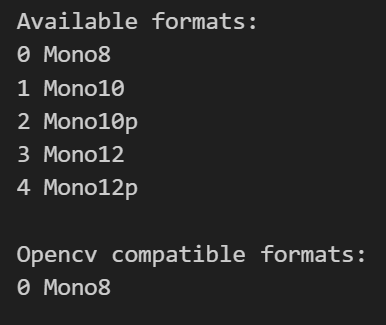
\includegraphics[scale=0.85]{assets/figures/Software/Format_Available.png}
    \caption{Compatible format results}
    \label{fig:Soft_Vimba_Format}
\end{figure}
Once the correct parameters have been displayed, simply call up this line of code, inserting the table cell corresponding
to the desired format (in this case, cell 0) :
\begin{verbatim}
    cam.set_pixel_format(opencv_formats[0])
\end{verbatim}
Once the connection to the camera has been made and the format has been set, our program will need to take images.
To do this, simply call the following function:
\begin{verbatim}
    frame = cam.get_frame().as_opencv_image()
\end{verbatim}
This function can be modified to suit individual requirements, and loops can be added to capture several images in succession.
%====================================================================================================
% The software
%====================================================================================================
\newpage
\section{The software}
\subsection{Principle}
In order to be able to output an image result, some programming is required. To do this, the program can be divided into 3 parts:
\begin{itemize}
    \item User interface : This part is not mandatory, but it makes the system much easier to use. It was therefore decided
          to include it in view of the system's extensive use. This part should include the entire measurement program,
          calibration and updating of camera parameters, and feedback on the measurement and its progress.
    \item Initialization : This program will initialize the system for future measurement.
          It would be interesting to be able to skip the initialization if several measurements are carried out in succession.
    \item Measurement : This is the system's key program. It performs the measurement and transforms the software data into user-readable data.
\end{itemize}
\begin{figure}[H]
    \centering
    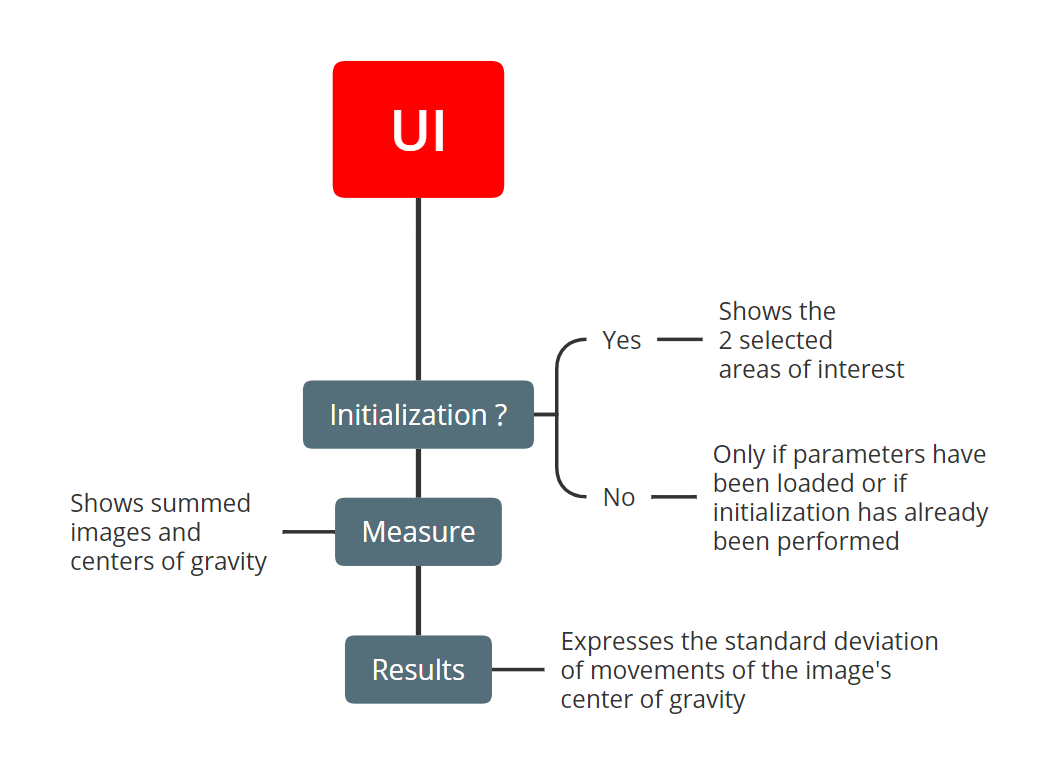
\includegraphics[scale=0.85]{assets/figures/Software/General.png}
    \caption{Software principle as seen by the user}
    \label{fig:Soft_General}
\end{figure}
Figure \ref{fig:Soft_General} shows the application's general operating principle. This application may be updated and changes
are to be expected after the first use in real conditions. It would also be interesting to work with potential future users
to optimize it for their needs.
\newpage
\subsection{Initialization}
The initialization program is essential for the measurement to run smoothly. It is also used to optimize the working
time of the measurement program by cropping only the necessary areas of the image. The basic principle of this program
can be seen in figure \ref{fig:Soft_Init}.
\begin{figure}[H]
    \centering
    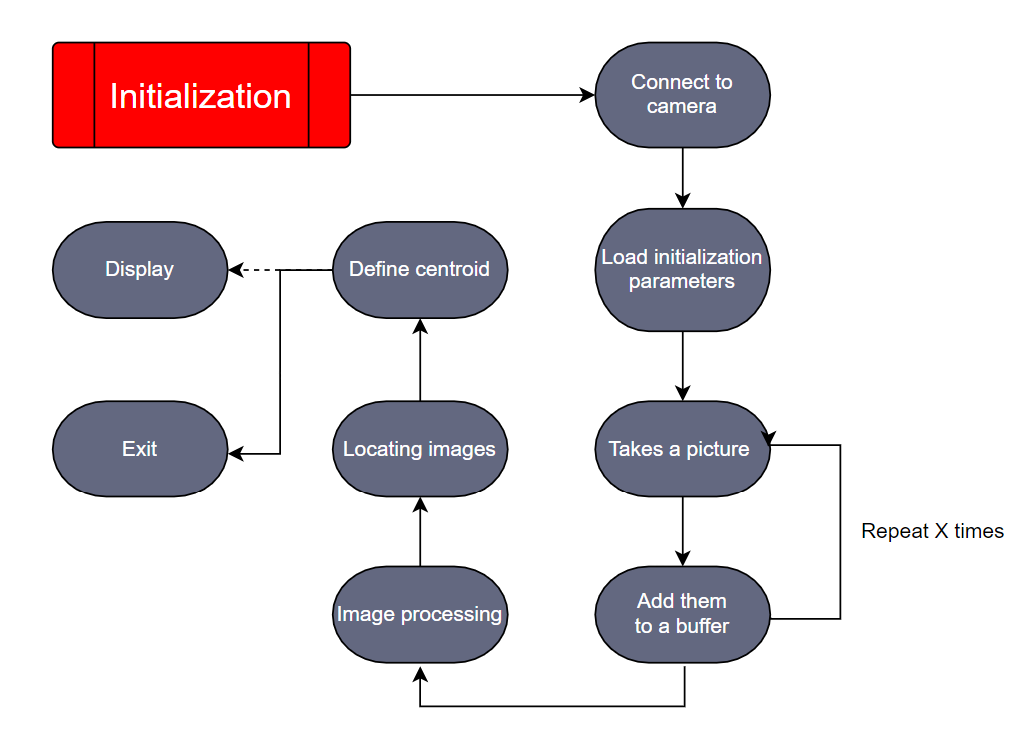
\includegraphics[scale=0.85]{assets/figures/Software/Initialization.png}
    \caption{Block diagram of the initialization function}
    \label{fig:Soft_Init}
\end{figure}
The initialization program performs the following steps :
\begin{enumerate}
    \item Camera connection
    \item Load initialization parameters (e.g. longer exposure time)
    \item Take several images to average out turbulence as far as possible (and as quickly as possible).
    \item Image adjustment (e.g.: clear defaults, increase contrast, etc.)
    \item Location of the 2 focal points of the image
    \item Find the centroid of each area of interest.
    \item Recover and save areas of interest for measurement (Crop image afterwards to reduce processing time)
    \item Display centers of interest if required.
\end{enumerate}
The program principle is the same for all languages. However, for reasons of time, image processing methods and
software accessibility, the program has been written in Python.
\newpage
\subsection{Measurement}
The measurement program is the heart of the system. It enables the measurement to be carried out and the results to be
processed into user-friendly values.The software principle is shown on the block diagram in figure \ref{fig:Soft_Meas}.
\begin{figure}[H]
    \centering
    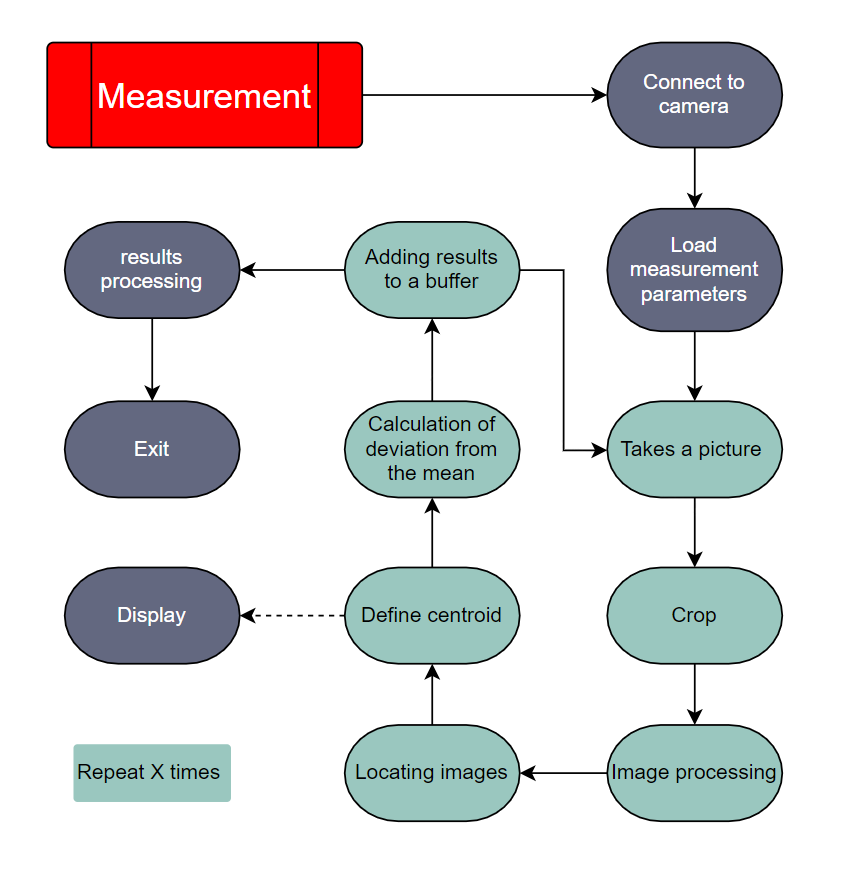
\includegraphics[scale=0.85]{assets/figures/Software/Measurement.png}
    \caption{Block diagram of the measurement function}
    \label{fig:Soft_Meas}
\end{figure}
Cropping the image will considerably reduce process time. The crop ratio will depend on the objects observed.
\bigbreak
The results process simply calculates the standard deviation of the centroid measurements taken.
\begin{equation}
    \sigma = \sqrt{\frac{1}{N}\sum\left(X-X_{init}\right)^2}
\end{equation}
This calculation can be performed for X and Y coordinates and for the total distance calculated using Pythagoras.
However, you'll need to express the standard deviation in arc-seconds using :
\textbf{\textcolor{red}{AJOUTER CALCUL}}
\newline
Once the standard deviation has been calculated, Fried's parameter can be determined by taking the coefficient $r_0$ out of
equation \ref{eq:Opti_Sigma}:
\begin{equation}
    r_0 = 0.1698^{3/5}*\left(\frac{\lambda}{\sigma}\right)^{6/5}*\left(\frac{1}{D}\right)^{1/5}
\end{equation}
\newpage
\subsection{User interface}
To facilitate the use of the system, it was decided to create a user interface.
This window will contain all the elements required to use the \Gls{DIMM}.
\begin{figure}[H]
    \centering
    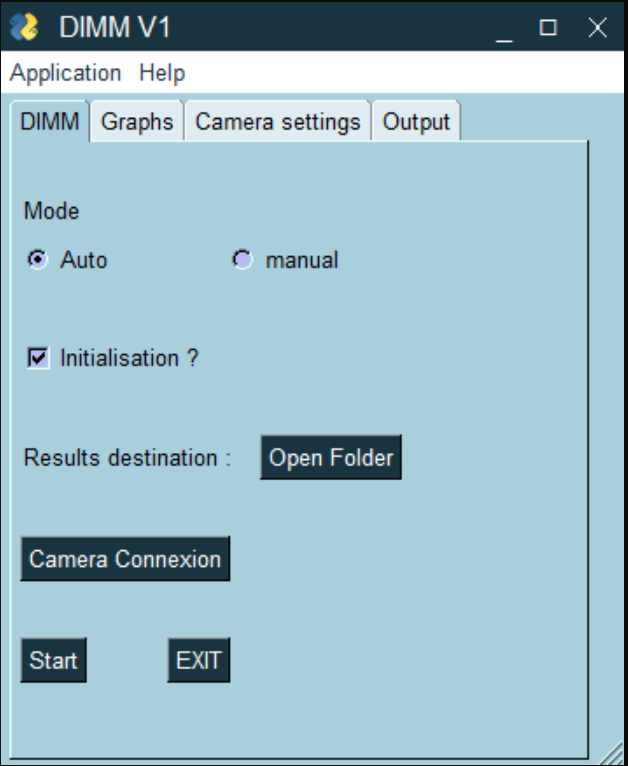
\includegraphics[scale=0.85]{assets/figures/Software/GUI1.png}
    \caption{User interface visualization}
    \label{fig:Soft_GUI}
\end{figure}
The first version of the user interface is shown in Figure \ref{fig:Soft_GUI}.
This application contains all options available for \Gls{DIMM} use :
\begin{itemize}
    \item "\Gls{DIMM}" page : This is the main part of the application. It allows you to select the measurement mode,
          whether the measurement needs to be initialized, the location of the results file and the camera connection test.
    \item "Graphs" page : This page will show the evolution of results over time.
    \item "Camera settings" page : This part of the application performs exactly the same functions as the VIMBA application.
          However, if parameters need to be adjusted in real time, it will be possible to modify them directly on the application.
          You can also use this page to save or load parameter files on your computer.
    \item "Output" page : This page will ensure that the image you have taken is the one you expected.
          The first measurement will be displayed in this section so that you can debug the system in the event of an error,
          or check the measurement if the result looks suspicious.
    \item The "help" section contains instructions for setting up the system.
\end{itemize}

\chapter{Global system}
\begin{figure}[H]
    \centering
    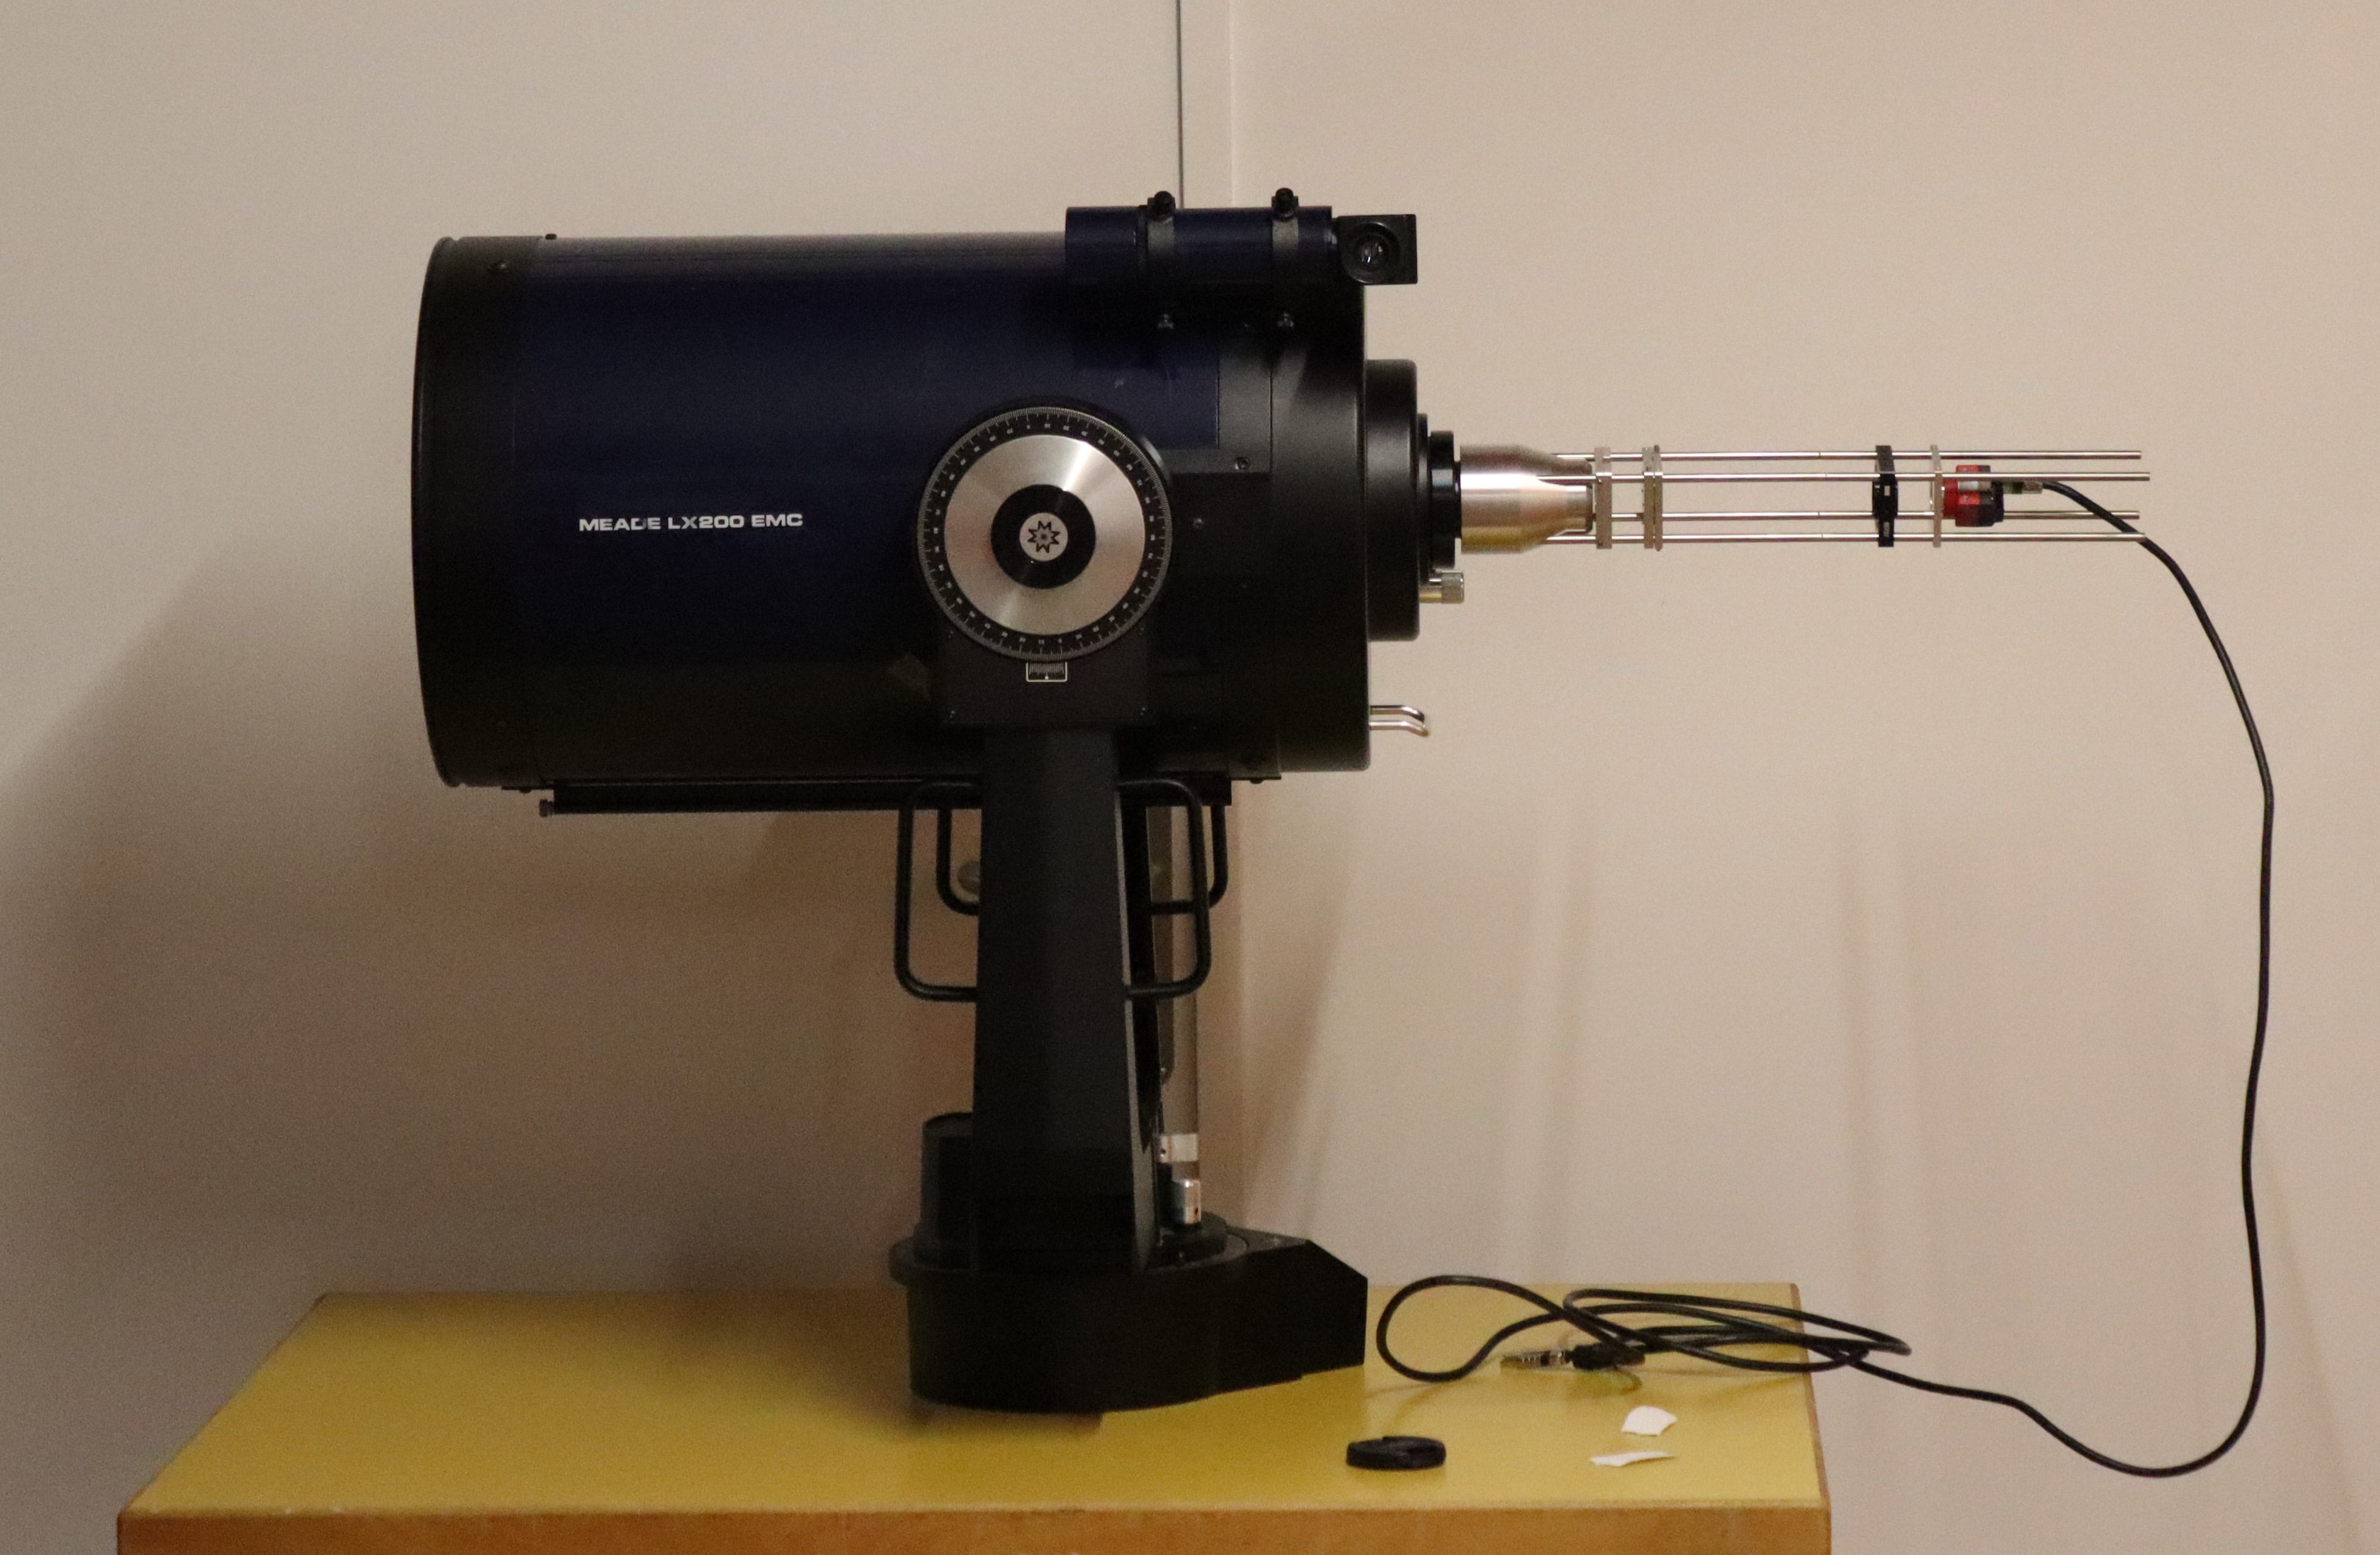
\includegraphics[scale=0.1]{assets/figures/System/IMG_5308.JPG}
    \caption{Mounted system}
    \label{fig:GLOB_Syst}
\end{figure}

\chapter{Measurement}
This section describes the measurements and image processing methods used to obtain the results.
\section{Image processing}\label{sec:MES_TIS}
First, the software needs to retrieve the camera image.
\begin{figure}[H]
    \centering
    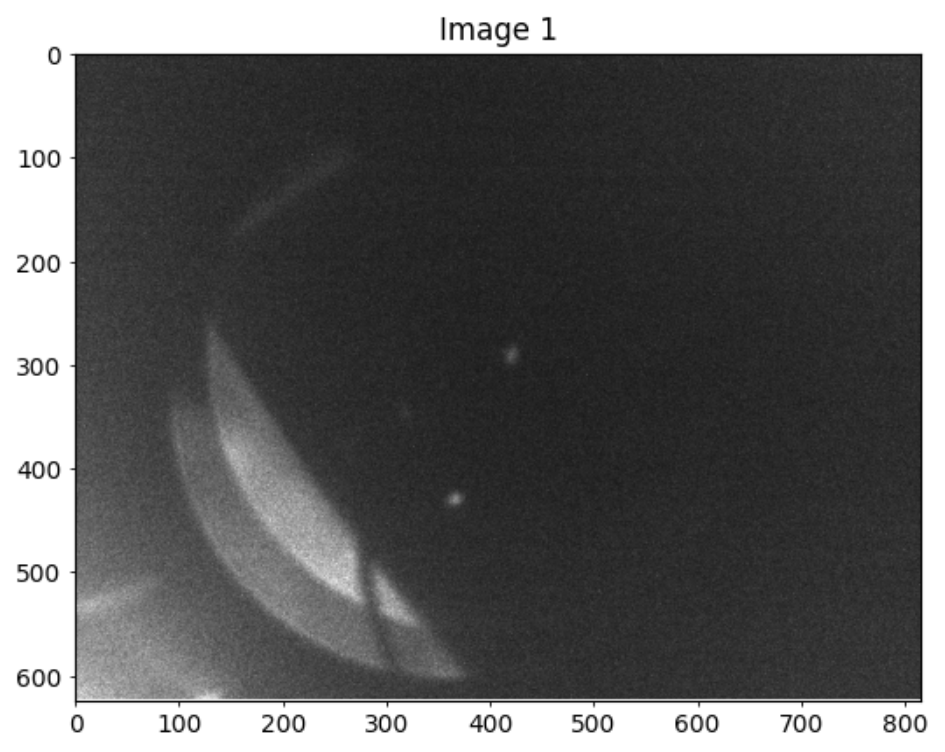
\includegraphics[scale=0.75]{assets/figures/MesuresResultats/ImageSimple.png}
    \caption{Image sent by the camera}
    \label{fig:MES_Ima1}
\end{figure}
An image is recovered using the camera (figure \ref{fig:MES_Ima1}). This image was taken on an "artificial" star, as the weather
was poor during the test phase. The two stars are easy to recognize.
\newpage
Next, a series of 100 images were recovered.
Once all 100 images had been taken, a visual check was carried out to validate the movement of the stars on the screen.
As the background disturbed the basic image (images taken during the day), it was decided to crop it around the
2 stars to remove the bright part (bottom left). The result is shown in Figure \ref{fig:MES_ImaMoy}.
\begin{figure}[H]
    \centering
    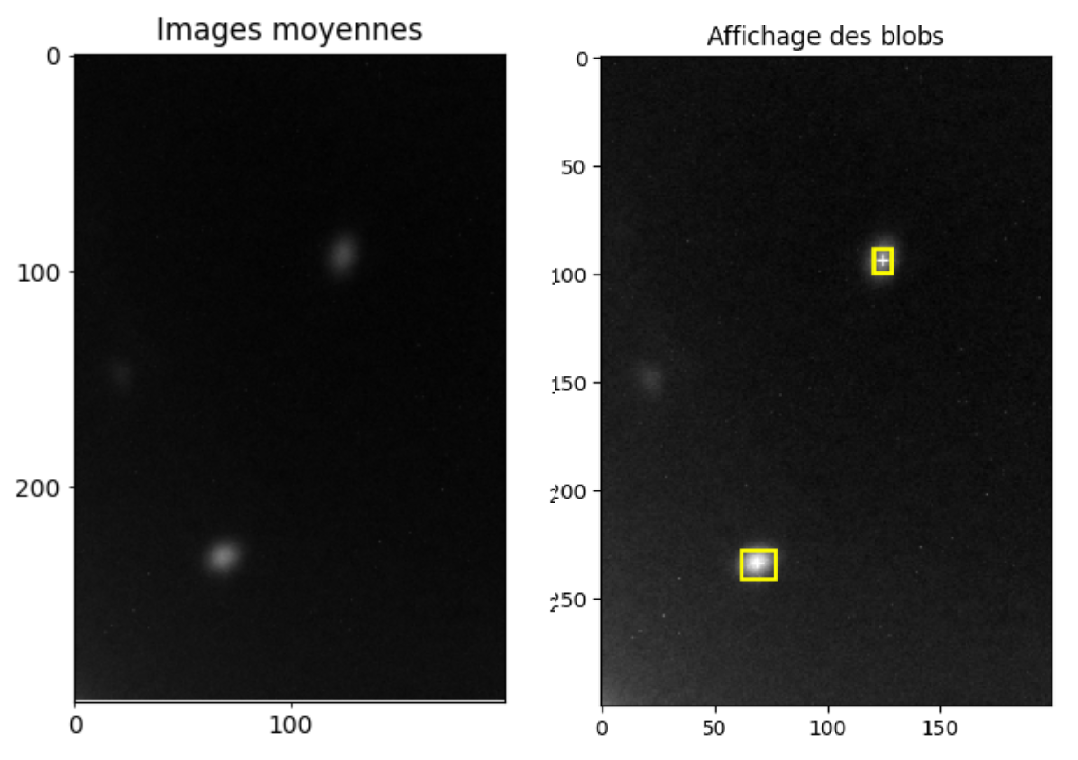
\includegraphics[scale=0.95]{assets/figures/MesuresResultats/ImageMoyenne.png}
    \caption{Addition of all images and star location}
    \label{fig:MES_ImaMoy}
\end{figure}
Figure \ref{fig:MES_ImaMoy} also shows the image used to initialize the system. It contains the 100 images summed and rescaled in values from 0 to 255.
The next step is to locate the 2 stars and find their centroid.
Once initialization is complete, the 2 centroids will be stored in memory, along with the star radius, so that they can
be differentiated.
\newpage
\section{Measurement}
The steps described above (Section \ref{sec:MES_TIS}) will then be carried out for each measurement image.
The stars must be located and their centroids determined (as shown in Figure \ref{fig:MES_ImaMoy}).
\begin{figure}[H]
    \centering
    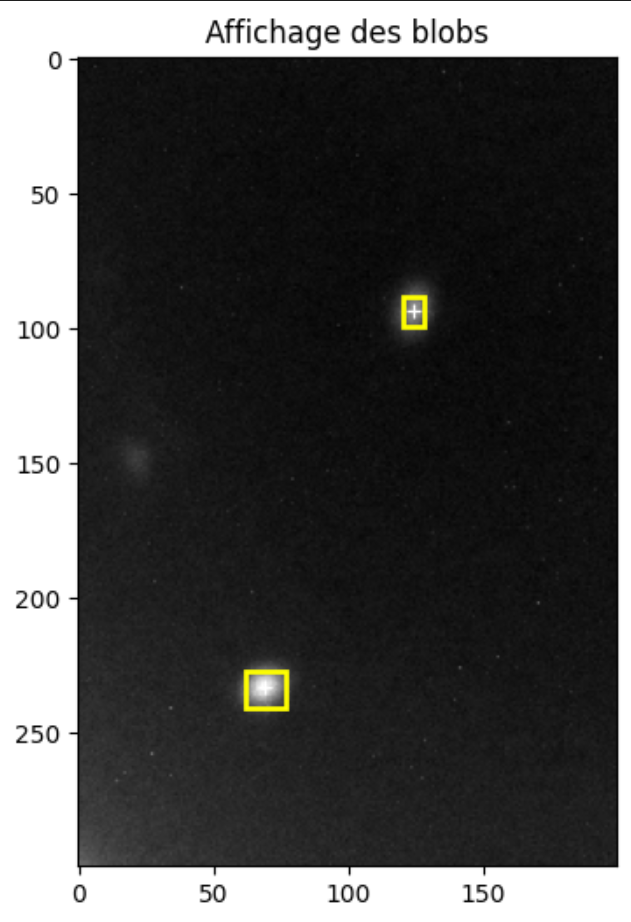
\includegraphics[scale=0.75]{assets/figures/MesuresResultats/BlobsInit.png}
    \caption{Image recognition}
    \label{fig:MES_ImaBlob}
\end{figure}
Each Centroid will be stored in a table specific to the corresponding star.
\newline
Recognition may not work correctly. In this case, the measurement is simply deleted.
However, it would be interesting to add an anomaly detection algorithm later on.
\newpage
\section{Results}
Once all the centroids have been recovered, simply convert them into micrometers to see how the star moves in relation to the turbulence.
\newline
The results of the variations according to the coordinates of the measurements are shown in Figure \ref{fig:MES_VarIm1} and Figure \ref{fig:MES_VarIm2}.
\begin{figure}[H]
    \centering
    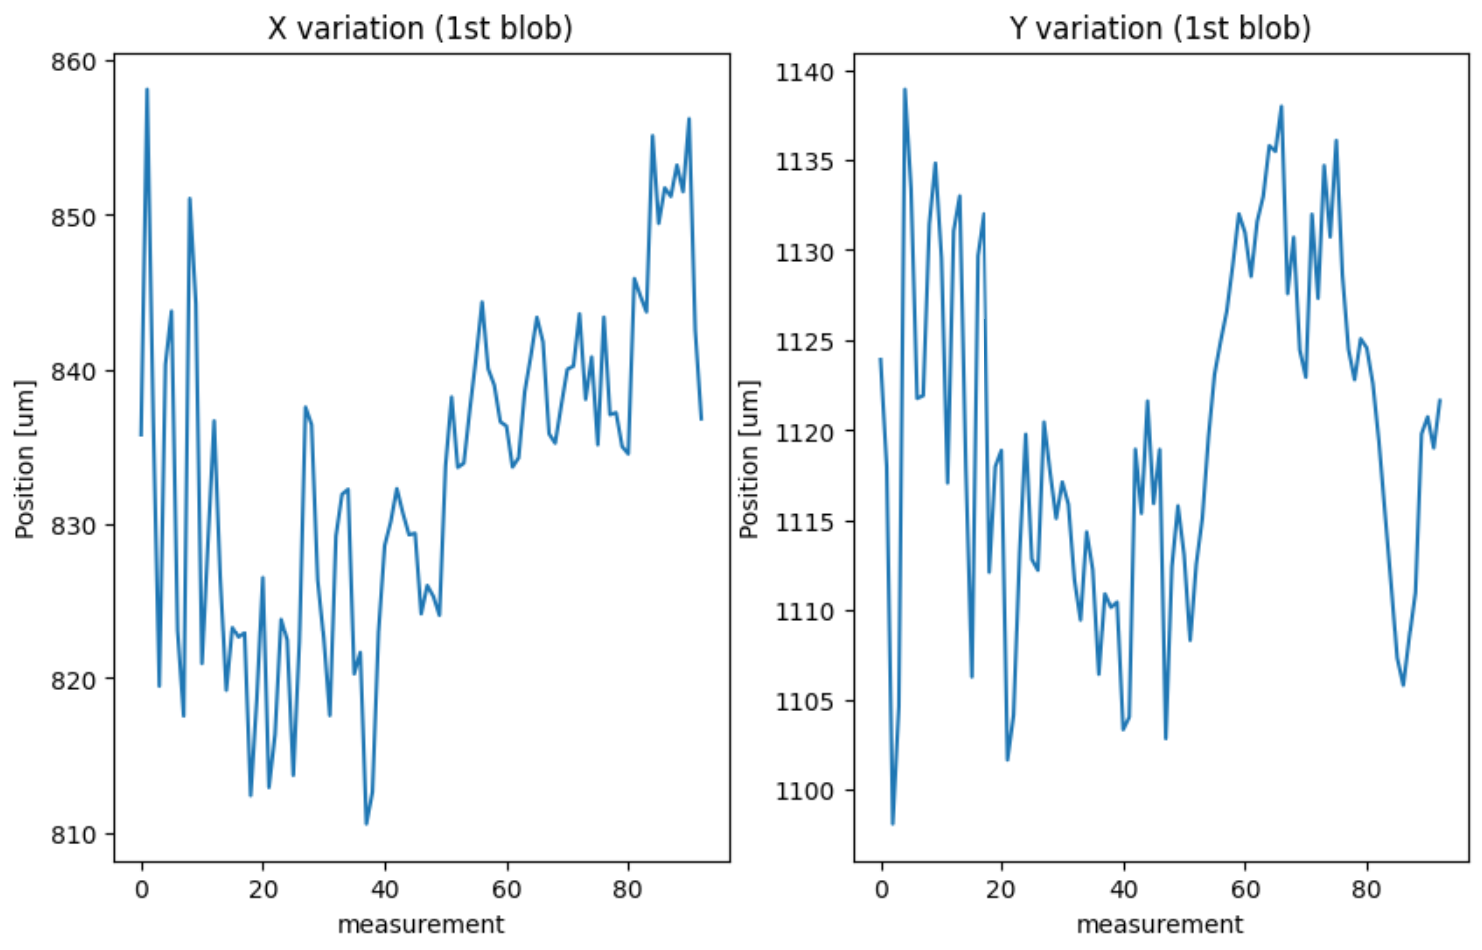
\includegraphics[scale=0.6]{assets/figures/MesuresResultats/VariationImage1.png}
    \caption{Coordinate variation (Image 1)}
    \label{fig:MES_VarIm1}
\end{figure}

\begin{figure}[H]
    \centering
    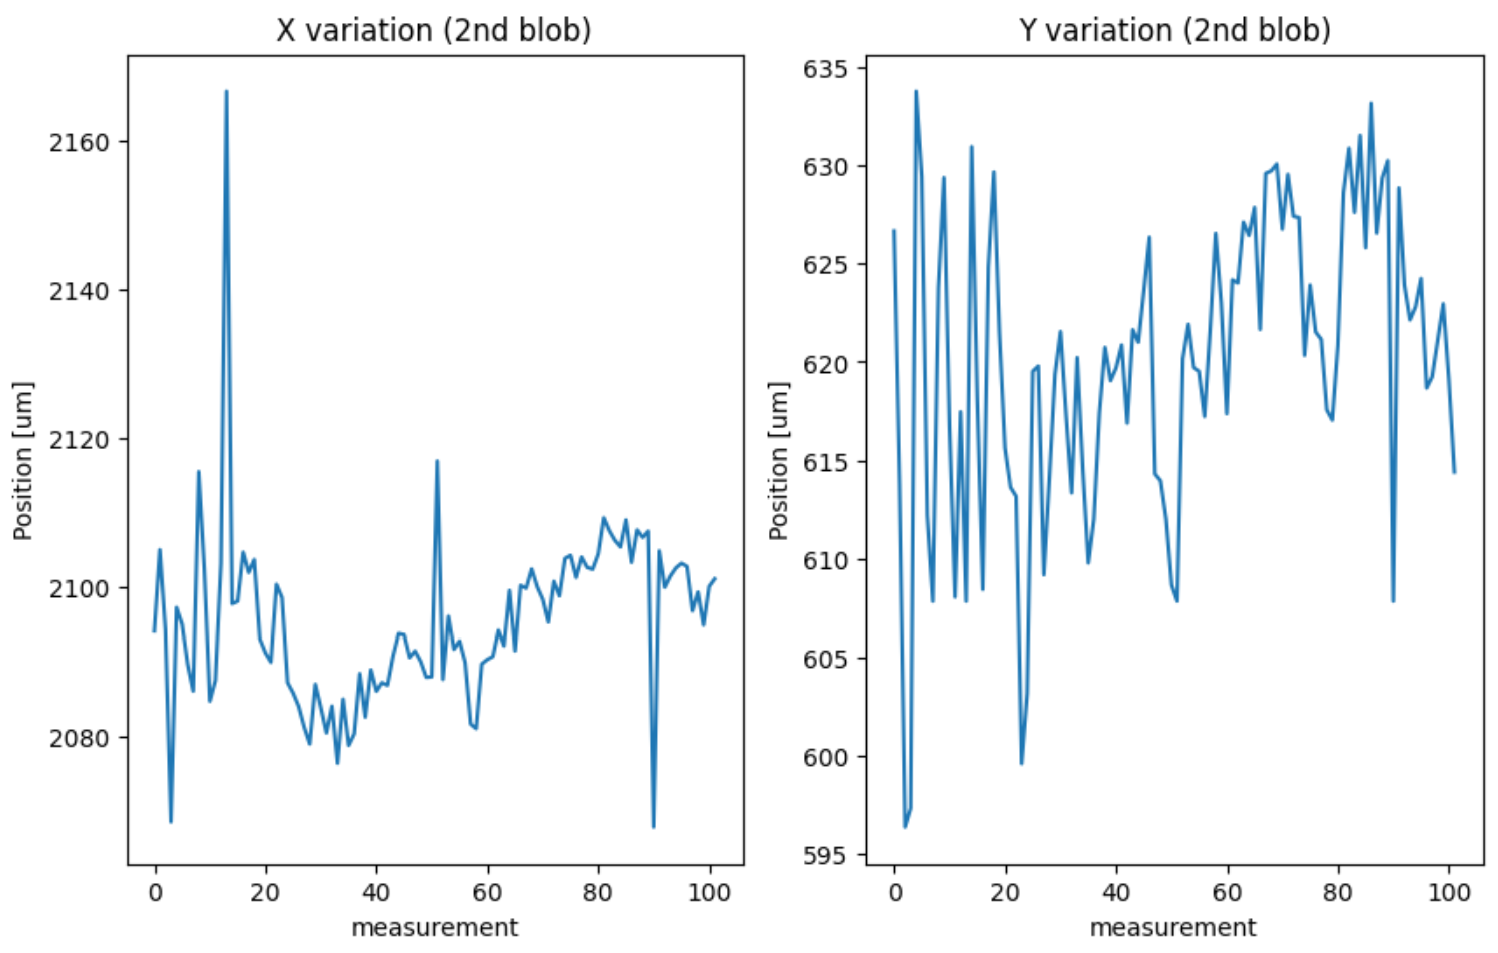
\includegraphics[scale=0.6]{assets/figures/MesuresResultats/VariationImage2.png}
    \caption{Coordinate variation (Image 2)}
    \label{fig:MES_VarIm2}
\end{figure}
\newpage
It's also interesting to represent the centroid of the 2 stars according to their position on the screen. 
In the 2 figures below (\ref{fig:MES_VarCenter1} and \ref{fig:MES_VarCenter2}), the initialization centroids are 
shown in blue and the measurement centroids in red.
\begin{figure}[H]
    \centering
    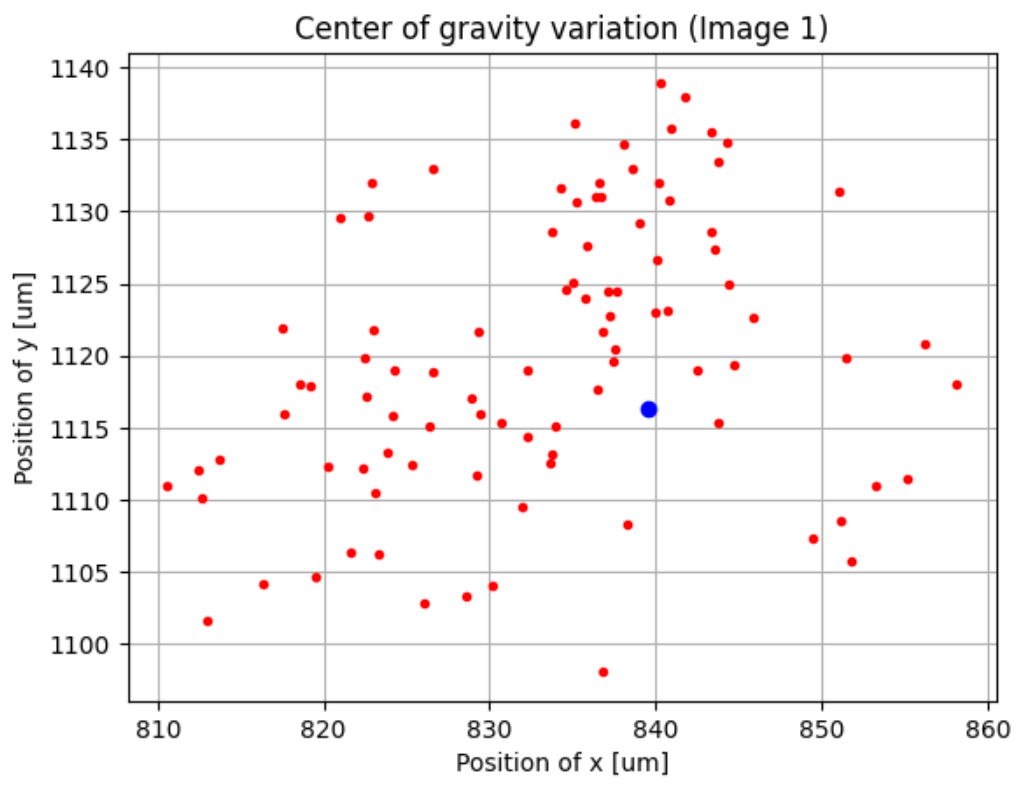
\includegraphics[scale=0.65]{assets/figures/MesuresResultats/VariationCenter1.png}
    \caption{Shifting centers of gravity (Image 1)}
    \label{fig:MES_VarCenter1}
\end{figure}

\begin{figure}[H]
    \centering
    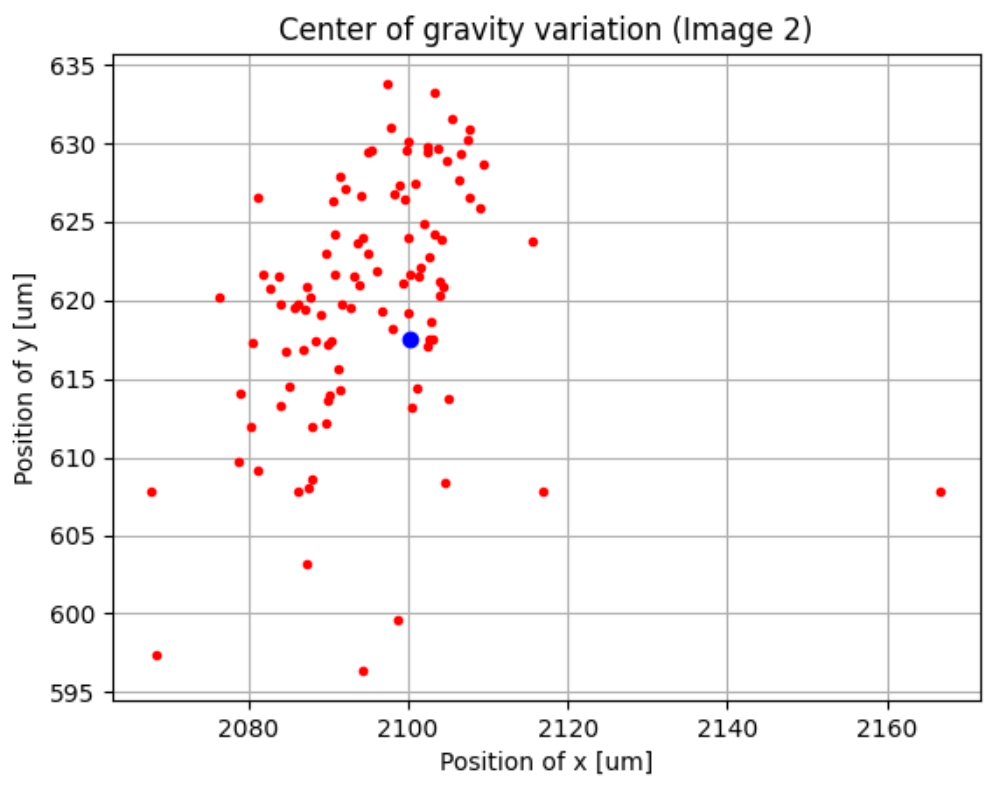
\includegraphics[scale=0.65]{assets/figures/MesuresResultats/VariationCenter2.png}
    \caption{Shifting centers of gravity (Image 2)}
    \label{fig:MES_VarCenter2}
\end{figure}
The measurements of the centroids in the second image have a value that seems out of line. It will therefore not be analyzed 
in the following section (\ref{sec:ANAL_Pos}). 
These errors may occur despite the protection implemented. 
This is due to the image processing and star recognition algorithms.
This algorithm will be modified to make it more reliable in the future. As it stands, however, it still contains a few bugs.

\chapter{Analysis}
\section{Qualitative analysis}\label{sec:ANAL_Pos}
As far as the mechanical and optical aspects of the project are concerned, the expected results are conclusive.
The mechanical part is usable, works properly and the system is adjustable.
As far as the optical part is concerned, after the preliminary tests carried out, the system is operating correctly.
The result shown in Figure \ref{fig:MES_Ima1} is the one expected and observed for all the measurements made.
\bigbreak
As for the measurement results, the graphs in figures \ref{fig:MES_VarCenter1} and \ref{fig:MES_VarCenter2} show that star
movements have been detected.
The displacement zone is also around the initialization centroid.
These results were expected and are very encouraging.
\newline
The next step is to calculate the standard deviation of these results, convert it into an angle (arc second) and output the associated
Fried parameter. Unfortunately, due to lack of time, this part has not yet been completed.
\newline
\textbf{\textcolor{red}{RAJOUTER ICI QQCH}}
\section{Quantitative analysis}
As things stand, enough can be done to achieve a conclusive result. However, image processing and selection methods could be optimized.
This optimization requires time and thorough testing with a large batch of measurements (as many different ones as possible).
\newline
Some measurements are still recognized as good when in fact they are not (Figure \ref{fig:MES_VarCenter2}).
It would therefore be interesting to be able to add anomaly detection to the measurements so as to avoid such results. \newline
However, the software delivered the expected results. Star detection and foreground processing are sufficient for preliminary tests.
It would be interesting to test a batch of images (e.g. 500) by splitting them into several parts to find out the accuracy limit
of the measurement.
\newpage
\section{Achievements and improvements}
\subsection{Achievements}
For the mechanical and optical parts, all the expected results were achieved. These results are listed below:
\begin{itemize}
    \item Optical development of the \Gls{DIMM} system
    \item Mechanical development of the \Gls{DIMM} system
    \item ZEMAX and SOLIDWORKS design of the system.
    \item Preparation of drawings for machining mechanical components.
    \item Design of the 12" MEADE telescope for the optics laboratory.
\end{itemize}
For the software part, the following objectives were achieved:
\begin{itemize}
    \item Creation of an image analysis program.
    \item Detection of the image area of interest.
    \item Separation of the 2 images.
    \item Centroid recovery for each image.
    \item Data retrieval and display.
\end{itemize}
\subsection{Improvements}
The software works correctly. However, there are a few improvements to be made and optimizations to be added once
a larger data set has been obtained. \newline
The enhancements required to keep the system running smoothly are listed below:
\begin{itemize}
    \item Detection of measurement anomalies.
    \item Image processing optimization.
    \item More reliable image processing (requires a large dataset).
    \item Addition and modification of the alghorithm for sunspot detection and seeing profil.
    \item Added alghorithm for transforming data into user-understandable values.
    \item Perform tests with different dataset sizes to find out the system's accuracy limits.
\end{itemize}
Improvements that would be accessory to the proper functioning of the system, but which would greatly help it and make it more reliable, are :
\begin{itemize}
    \item Measurement alghoritms added to user interface.
    \item Addition of functions necessary for user understanding of data analysis.
          (For example: adding graphs, tracking measurements, saving measurements and vision parameters)
    \item Addition of pre-implemented measurement parameters.
          (After several tests, it would be interesting to pre-program measurement profiles for each measurable star).
\end{itemize}

\chapter{Conclusion}


\vfil
\hspace{8cm}\makeatletter\@author\makeatother\par
\hspace{8cm}\begin{minipage}{5cm}
    % Place pour signature numérique
    \printsignature
\end{minipage}

\clearpage
% \printbibliography
\chapter*{Bibliography}
\addcontentsline{toc}{chapter}{Bibliography}
|1| L.Jolissaint, "Optique adaptative au foyer d'un télescope de la classe 1 mètre", M.S. thesis, Geneva: 2001, 2001.
\bigbreak
|2| IRSOL, "Research activity: Research activity at irsol", [Online]. \newline Available: \hyperlink{IRSOL website}{https://www.irsol.usi.ch/research/research-activity/}. (accessed: 24.07.2023).
\bigbreak
|3| Sarazin, M., & Roddier, F., "The ESO differential image motion monitor", Astronomy and Astrophysics, 1990, (pages 294 to 300).
\bigbreak
|4| Edmund optics, [Online]. Available: \hyperlink{Edmund optics website}{https://www.edmundoptics.eu/}. (accessed: 17.07.2023).
\bigbreak
|5| Astroshop, "MAEDE solar filter 1375", [Online]. Available: \hyperlink{Astroshop website}{https://www.astroshop.de/fr/filtres-en-verre-montes/meade-filtre-solaire-1375-id-349-mm/p,59498}. (accessed: 17.07.2023).
\bigbreak
|6| L.Jolissaint, "Introduction à l'optique pour les ingénieurs", Course theory, HEIG-VD: 2023, 2023.

\label{glossaire}
\printnoidxglossary
\label{index}
\printindex

\appendix
\appendixpage
\addappheadtotoc

%====================================================================================================
% MEP Perso
%====================================================================================================
\chapter{Personnal drawing}
% ============================================ Adapter ==============================================
\label{App:MEP}
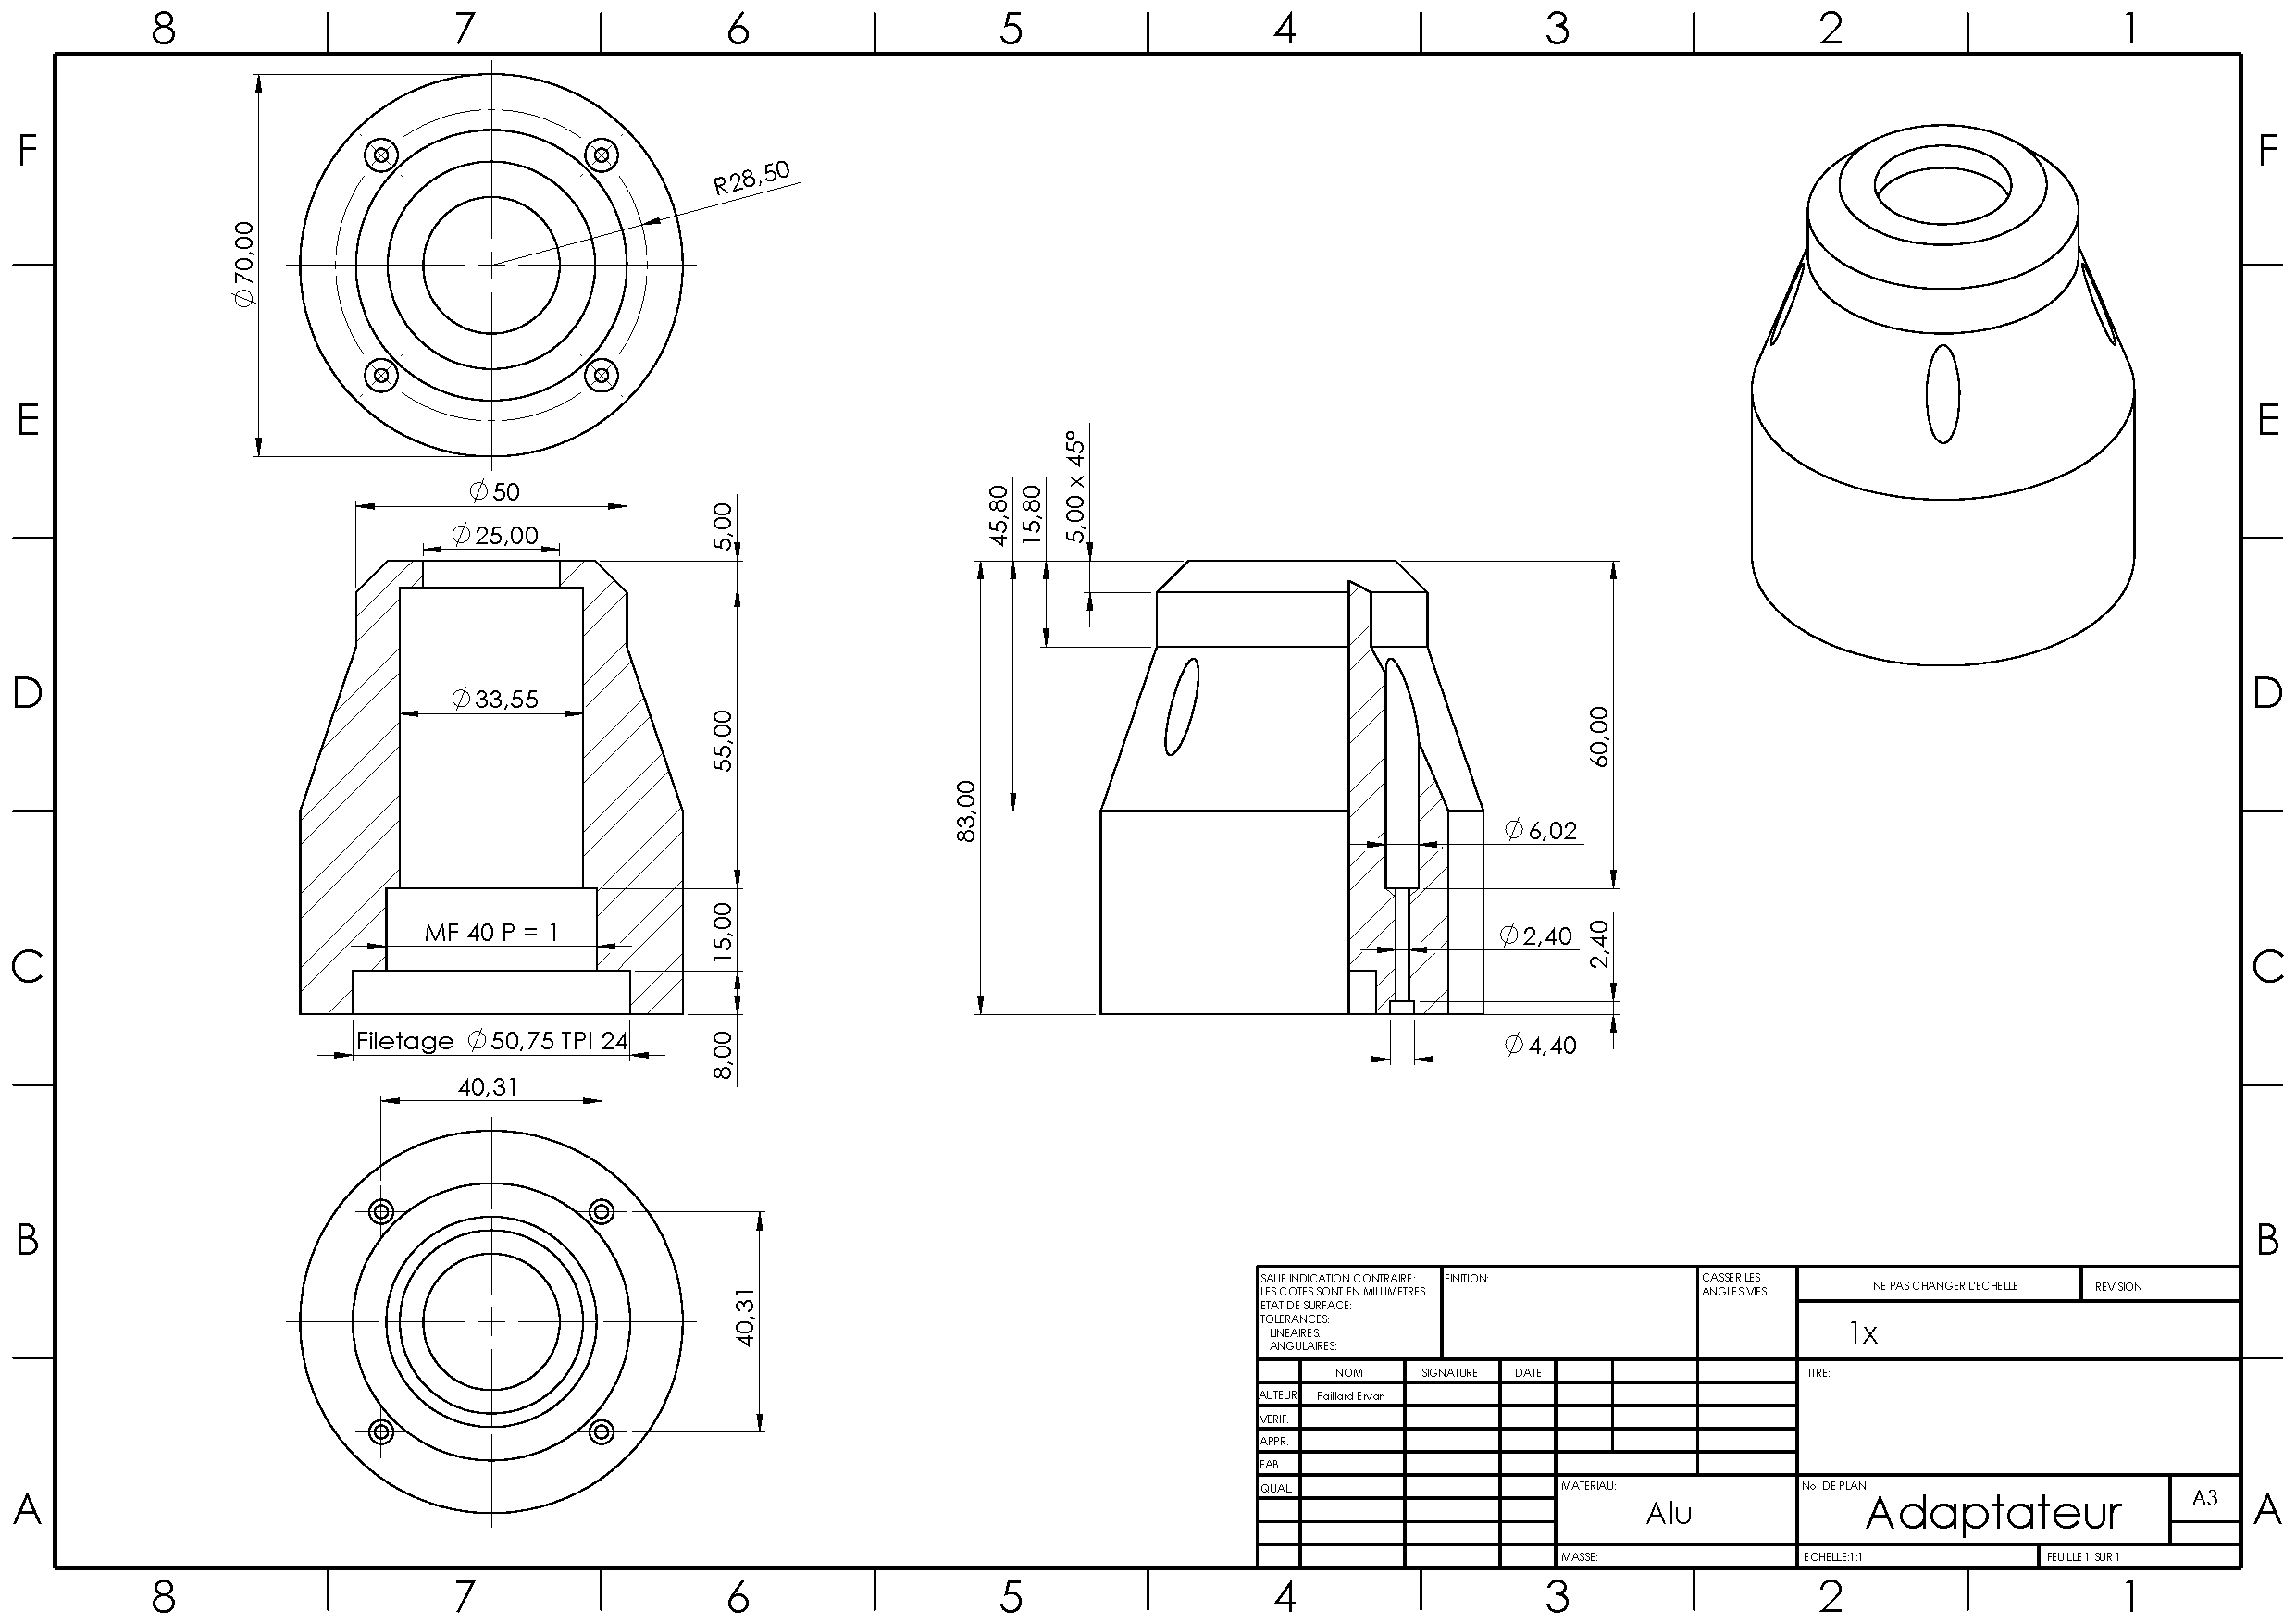
\includepdf[pages=-,angle=90,scale =0.9]{assets/Annexes/MEP/Adaptateur - Feuille1.pdf}
\newpage
% ========================================= Occulare screw ==========================================
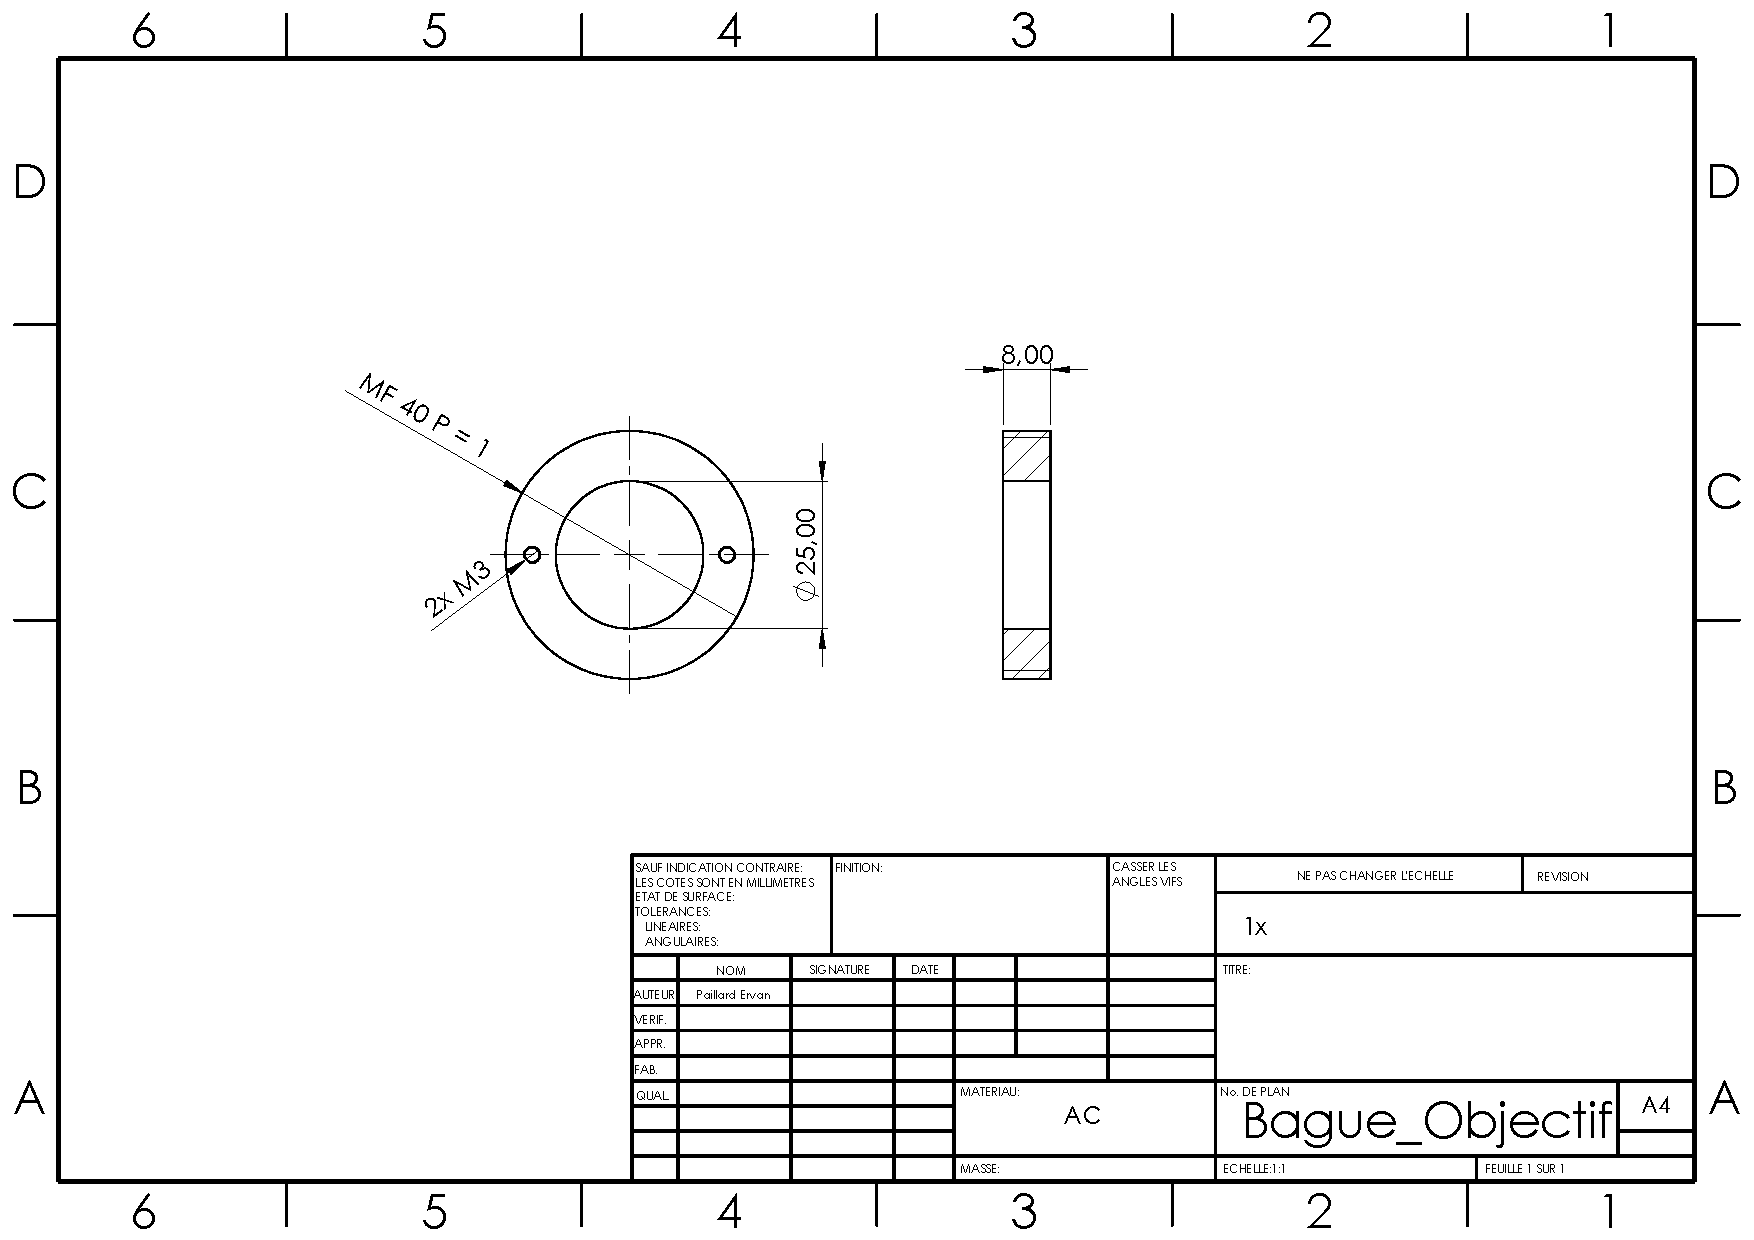
\includepdf[pages=-,angle=90,scale =0.9]{assets/Annexes/MEP/Bague_Objectif - Feuille1.pdf}
\newpage
% ========================================= Occulare screw ==========================================
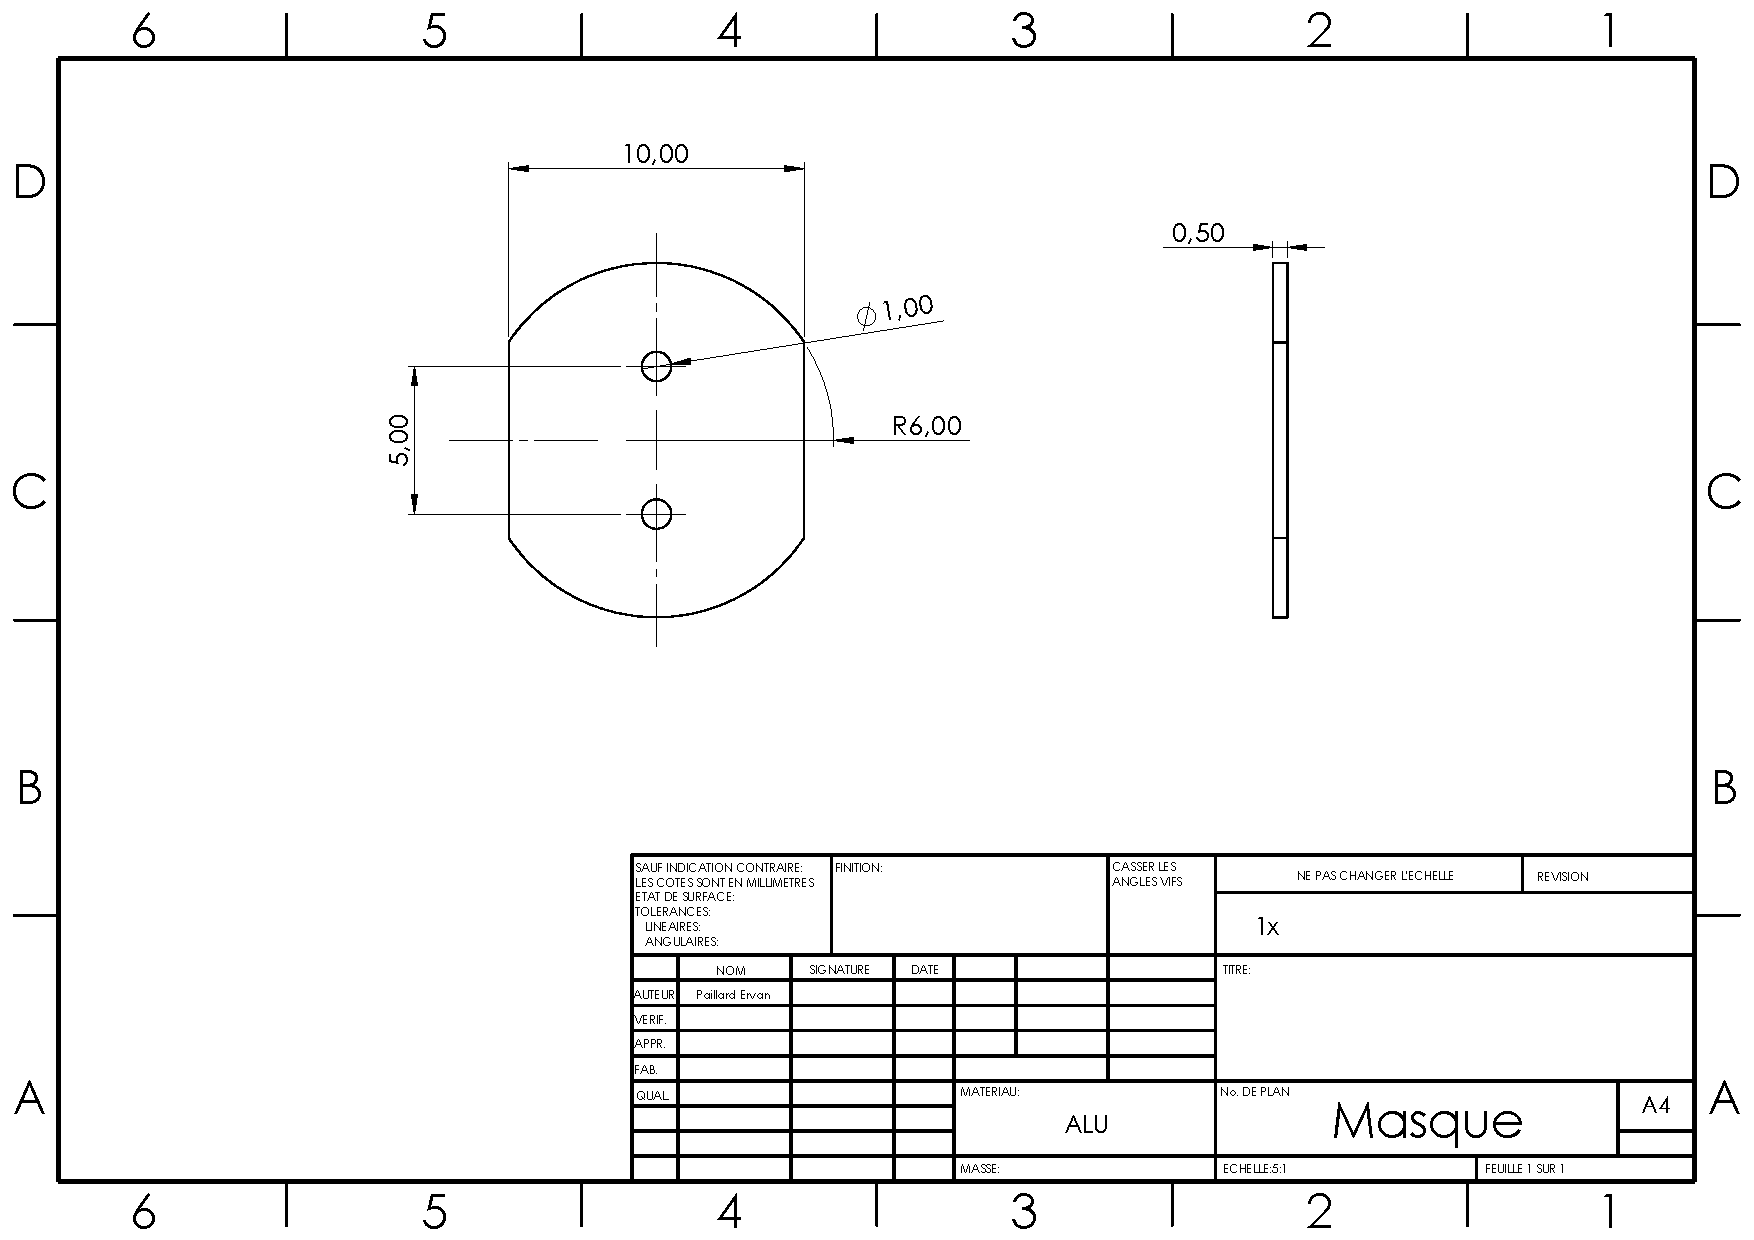
\includepdf[pages=-,angle=90,scale =0.9]{assets/Annexes/MEP/Masque - Feuille1.pdf}
\newpage
% ========================================= Occulare screw ==========================================
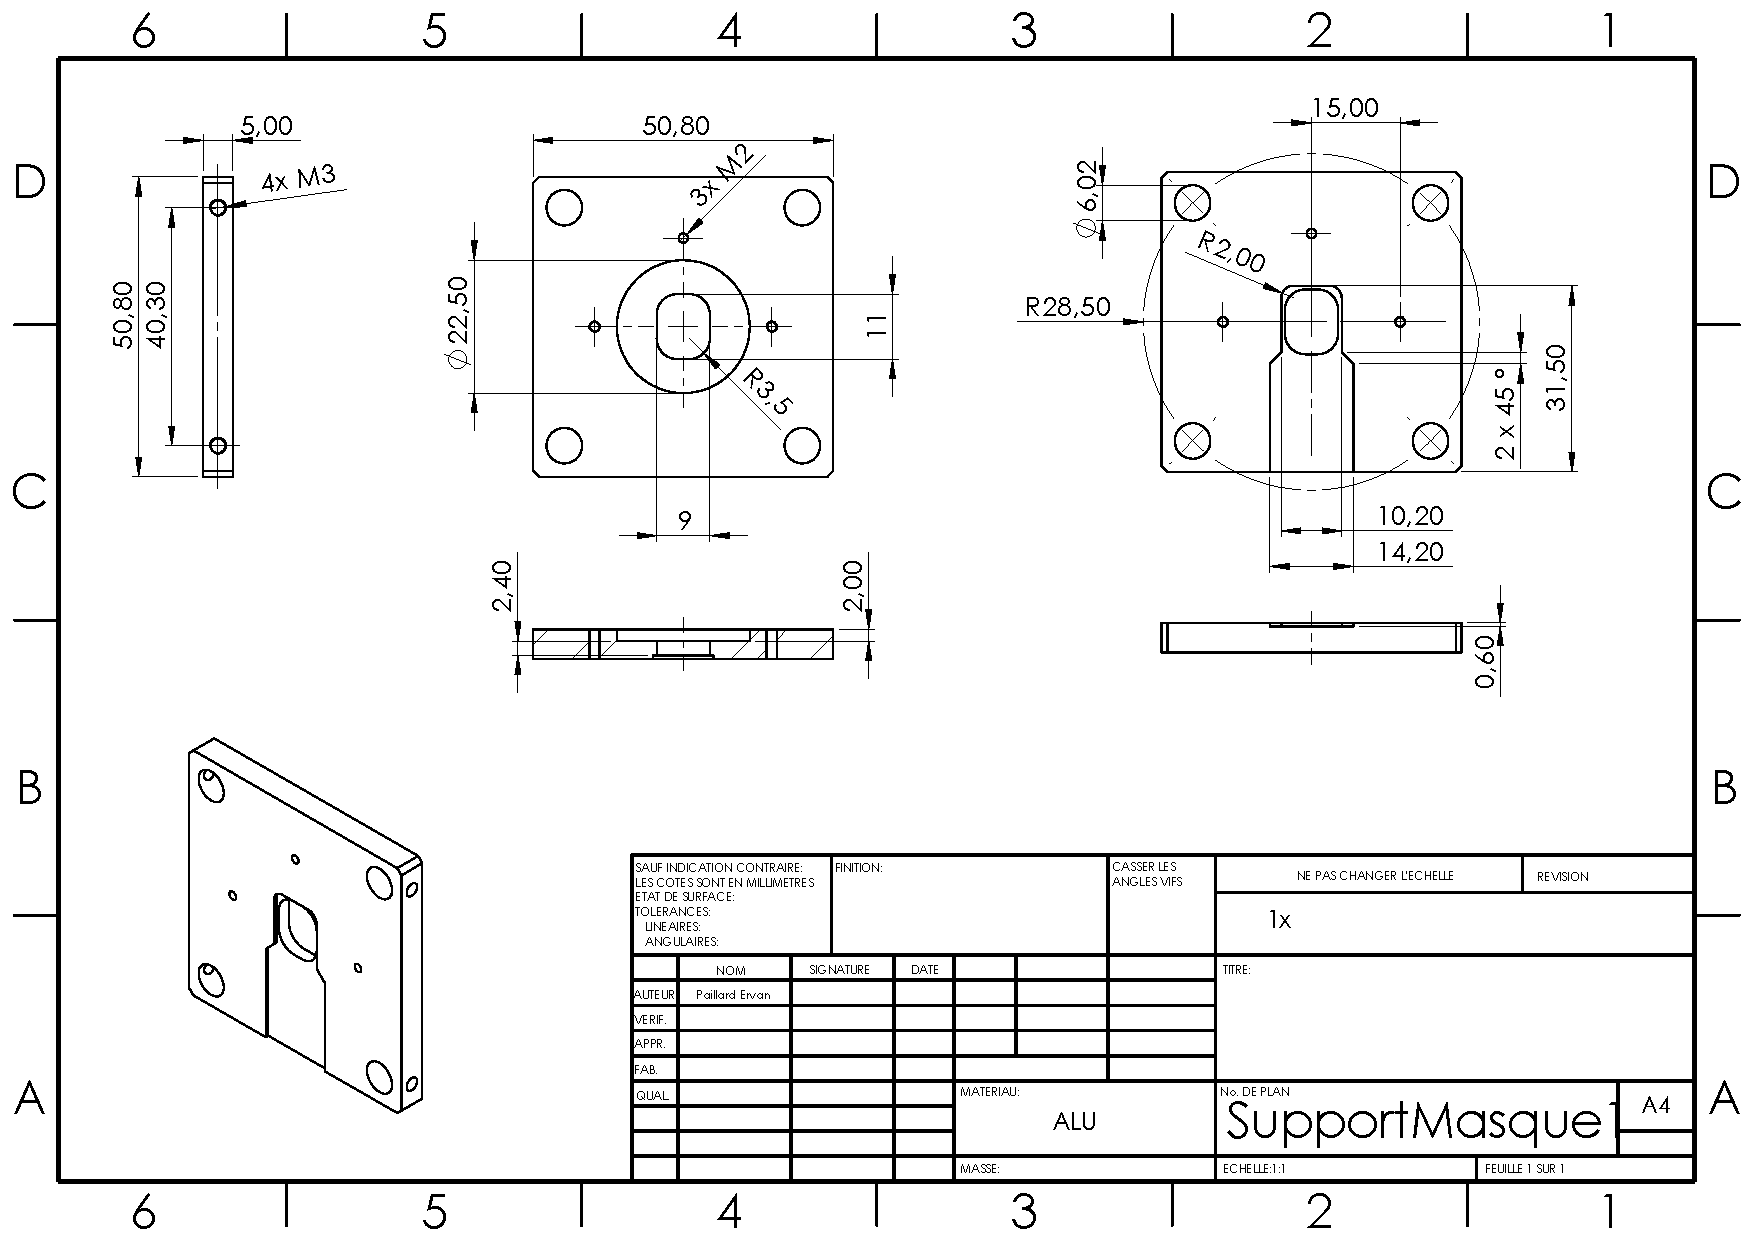
\includepdf[pages=-,angle=90,scale =0.9]{assets/Annexes/MEP/SupportMasque1 - Feuille1.pdf}
\newpage
% ========================================= Occulare screw ==========================================
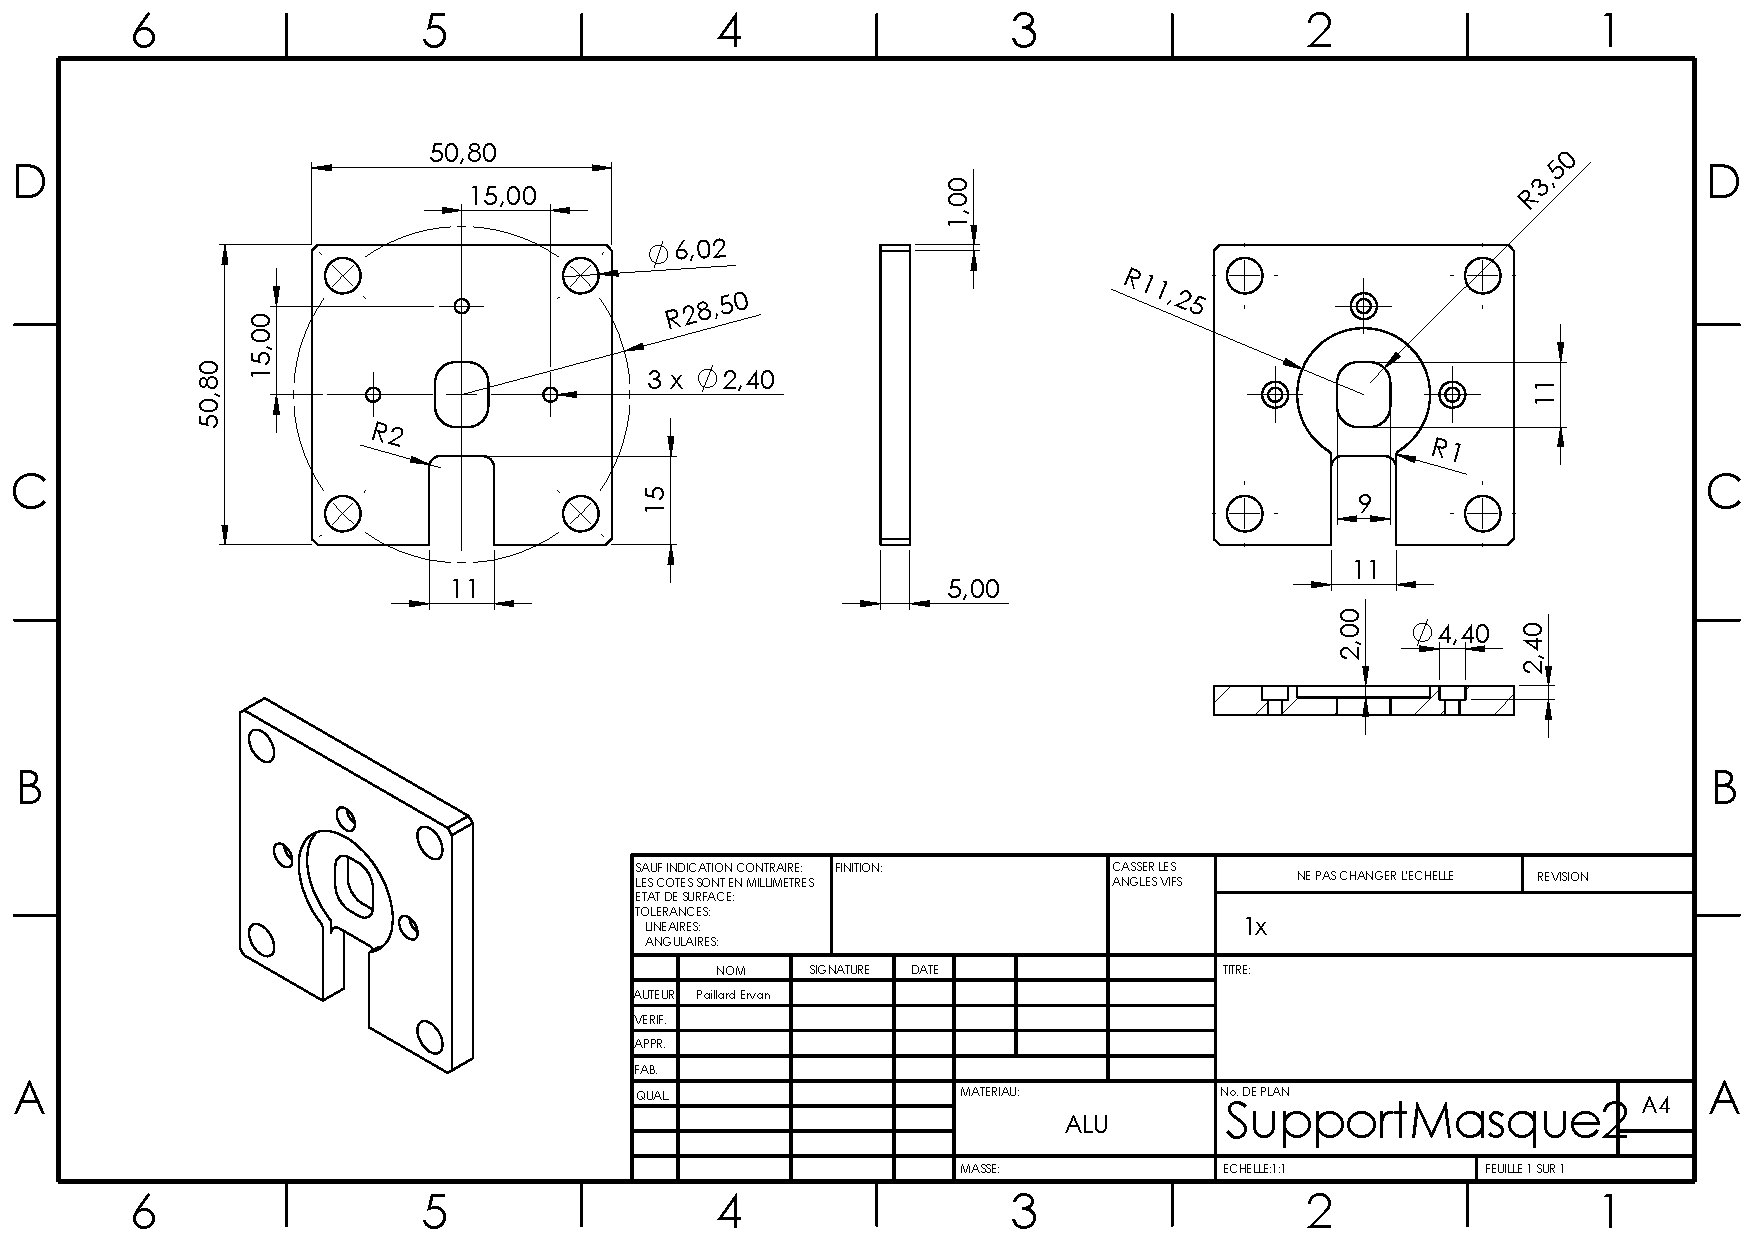
\includepdf[pages=-,angle=90,scale =0.9]{assets/Annexes/MEP/SupportMasque2 - Feuille1.pdf}
\newpage
% ========================================= Occulare screw ==========================================
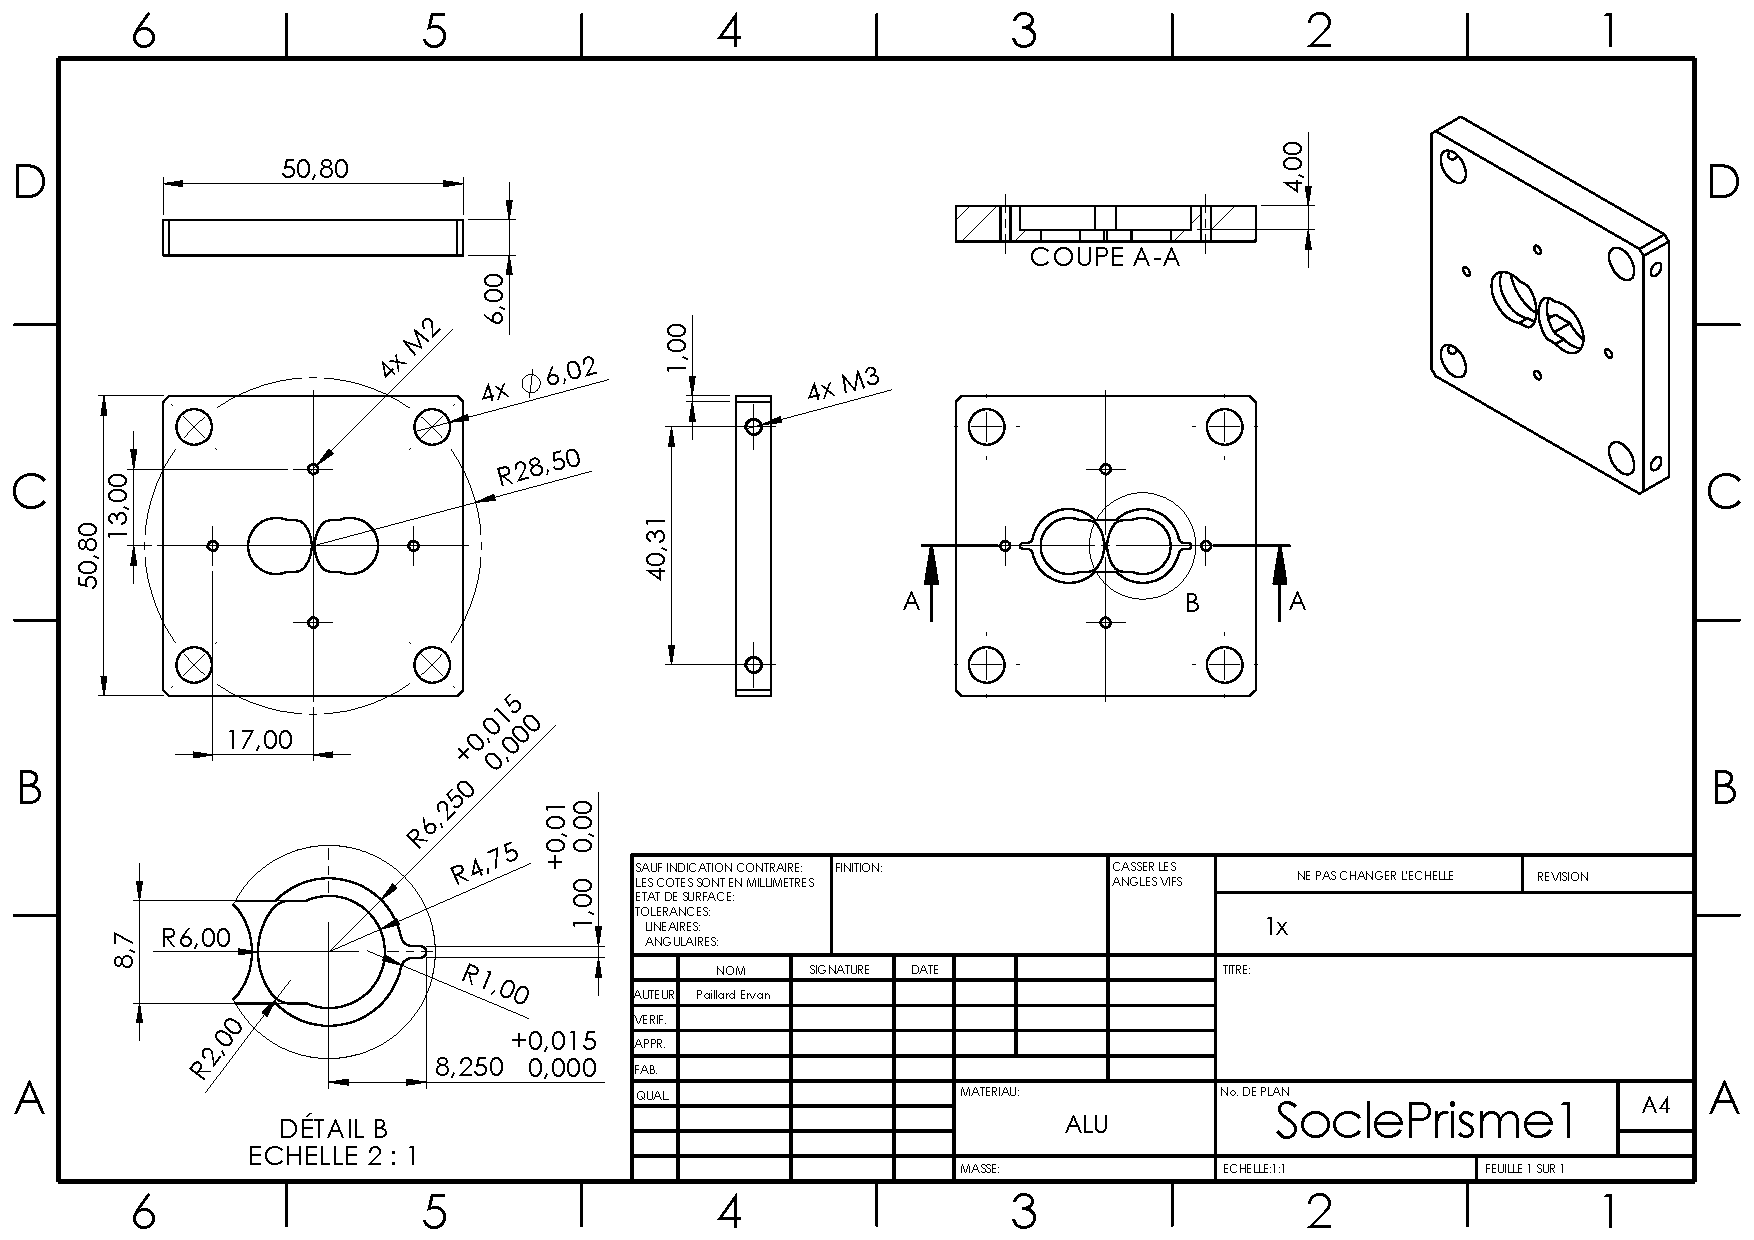
\includepdf[pages=-,angle=90,scale =0.9]{assets/Annexes/MEP/SoclePrisme1 - Feuille1.pdf}
\newpage
% ========================================= Occulare screw ==========================================
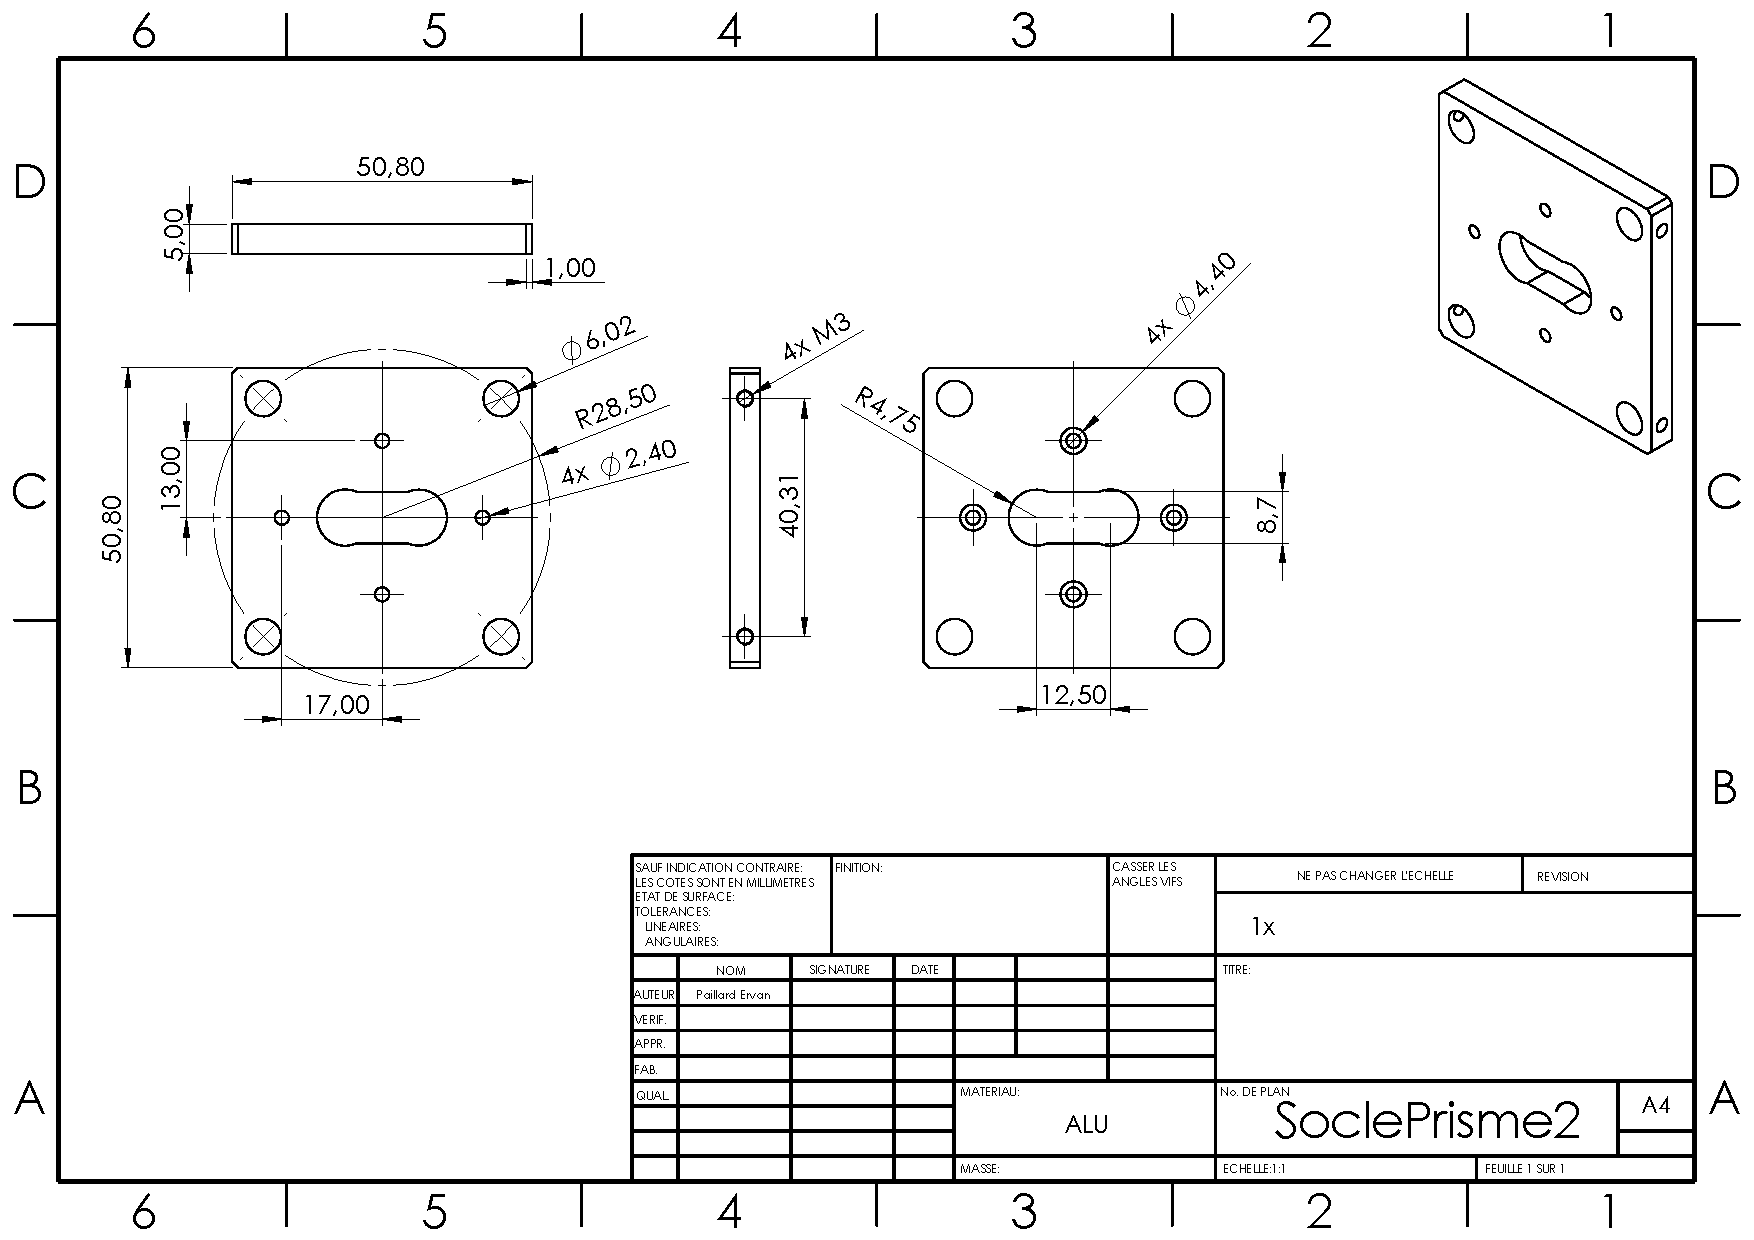
\includepdf[pages=-,angle=90,scale =0.9]{assets/Annexes/MEP/SoclePrisme2 - Feuille1.pdf}
\newpage
% ========================================= Occulare screw ==========================================
\includepdf[pages=-,angle=90,scale =0.9]{assets/Annexes/MEP/MaintientPrisme - Feuille.pdf}
\newpage
% ========================================= Occulare screw ==========================================
\includepdf[pages=-,angle=90,scale =0.9]{assets/Annexes/MEP/SupportCamera - Feuille1.pdf}
\newpage

%====================================================================================================
% EDMUND MEP
%====================================================================================================
\chapter{Edmund optics components drawing}
% ========================================= Occulare screw ==========================================
\includepdf[pages=-,angle=90,scale =0.9]{assets/Annexes/MEP Edmund/Prism.pdf}
\newpage
% ========================================= Occulare screw ==========================================
\includepdf[pages=-,angle=90,scale =0.9]{assets/Annexes/MEP Edmund/Lens.pdf}
\newpage
% ========================================= Occulare screw ==========================================
\includepdf[pages=-,angle=90,scale =0.9]{assets/Annexes/MEP Edmund/Support_Lens.pdf}
\newpage
% ========================================= Occulare screw ==========================================
\includepdf[pages=-,angle=90,scale =0.9]{assets/Annexes/MEP Edmund/Support_Lens2.pdf}
\newpage
% ========================================= Occulare screw ==========================================
\includepdf[pages=4,scale =0.9]{assets/Annexes/MEP Edmund/Camera.pdf}
\newpage

%====================================================================================================
% Other components
%====================================================================================================
\chapter{Datasheet of all other components}
% ========================================= Occulare screw ==========================================
\includepdf[pages=1-3,scale =0.9]{assets/Annexes/MEP Edmund/Camera.pdf}
\newpage

% Le colophon est le dernier élément d'un document qui contient des notes de l'auteur concernant la mise en page et l'édition du document : il est parfaitement optionnel.
% \input{colophon.tex}

\end{document}
